\listfiles
\documentclass[manuscript, review, screen]{acmart}
%\setcitestyle{super,sort&compress}
\citestyle{acmauthoryear}
\usepackage{booktabs} % For formal tables

\usepackage[ruled]{algorithm2e} % For algorithms
\usepackage{enumitem}

\graphicspath{{Images/}}
\usepackage{graphicx}

% Metadata Information

\acmYear{2017}
\acmMonth{3}

%\acmBadgeL[http://ctuning.org/ae/ppopp2016.html]{ae-logo}
%\acmBadgeR[http://ctuning.org/ae/ppopp2016.html]{ae-logo}

% Copyright
%\setcopyright{acmcopyright}
%\setcopyright{acmlicensed}
%\setcopyright{rightsretained}
%\setcopyright{usgov}
%\setcopyright{usgovmixed}
%\setcopyright{cagov}
%\setcopyright{cagovmixed}

% DOI
\acmDOI{0000001.0000001}


% Document starts
\begin{document}
% Title portion
\title{Nontrivial behavior of the fixed-point version of $2D$-chaotic maps} 
% \titlenote{This is a titlenote}
% \subtitle{This is a subtitle}
% \subtitlenote{Subtitle note}
\author{L. De Micco}

\email{ldemicco@fi.mdp.edu.ar}
\author{M. Antonelli}
\author{H. A. Larrondo}
\affiliation{%
  \institution{ICYTE (Instituto de Investigaciones Cient\'ificas y Tecnol\'ogicas en Electr\'onica)}
  \department{School of Engineering}
}
\affiliation{%
  \institution{CONICET ( Consejo  Nacional de
Investigaciones Cient\'{\i}ficas y T\'ecnicas)}}
%\author{M. Antonelli}
%\affiliation{%
%  \institution{ICYTE (Instituto de Investigaciones Cient\'ificas y Tecnol\'ogicas en Electr\'onica)}
%  \department{School of Engineering}
%}
%\author{H. A. Larrondo}
%\affiliation{%
%  \institution{ICYTE (Instituto de Investigaciones Cient\'ificas y Tecnol\'ogicas en Electr\'onica)}
%  \department{School of Engineering}
%}
%\affiliation{%
%  \institution{CONICET}}
%  

\begin{abstract}
This paper deals with a family of interesting $2D$-quadratic maps
 proposed by Sprott, in his seminal paper \cite{Sprott1993},
related to ``chaotic art".  Only results for the analytical representation of these
maps have been published in the open literature. Our main interest about these maps is
they may be used to generate a novel encryption system, because
they present multiple chaotic attractors depending on the selected
point in the parameter's space. Consequently the objective of
this paper is to extend the analysis to the digital version, to make
possible  the hardware implementation in a digital medium, like field programmable gate arrays (FPGA) in fixed-point arithmetic.
Our main contributions are: (a) the study of the domains of attraction in fixed-point arithmetic; (b)  the determination of the \textsl{threshold} of the bus width that preserves the integrity of the domain of
attraction and (c) the comparison between two quantifiers based on respective probability distribution functions and  the well known maximum Lyapunov exponent (MLE) to detect the above mentioned threshold. 
\end{abstract}



\keywords{2D-quadratic map's digitalization, randomness quantifier, fractional length, chaotic map's degradation}


%\thanks{This work is supported by the National Science Foundation,
%  under grant CNS-0435060, grant CCR-0325197 and grant EN-CS-0329609.
%
%  Author's addresses: G. Zhou, Computer Science Department, College of
%  William and Mary; Y. Wu {and} J. A. Stankovic, Computer Science
%  Department, University of Virginia; T. Yan, Eaton Innovation Center;
%  T. He, Computer Science Department, University of Minnesota; C.
%  Huang, Google; T. F. Abdelzaher, (Current address) NASA Ames
%  Research Center, Moffett Field, California 94035.}


\maketitle

%


\section{Introduction} \label{sec:intro}

% ==================================================
% resumen
%% LO QUE VAMOS A CONTAR EN ESTE PAPER ES LO SIGUIENTE:
%primero mostramos algunos atractores en flotante
%para uno de esos a tractores mostramos los dominios de atracci—n
%
%segundo contamos como estudiamos la degradaci—n de los dominios de atracci—on.
%tercero contamos como estudiamos la degradaci—n de las variables de estado del sistema, es decir de la serie temporal generada por el sistema
%cuarto contamos como implementamos
%mostramos los resultados concretos obtenidos para la degradaci—n de los dominios de atracci—n y para la degradaci—n de las variables de estado
% ==================================================
%

Chaotic systems have an increasing number of applications and their implementation is specially involved due to the \textsl{extreme sensitivity to initial conditions} that present. In general, 
these systems are used for the generation of controlled noises, these digital pseudo-random noise generators (PRNGs) 
can be employed in a large number of electronic applications, such as encryption sequences for privacy, multiplexing techniques, 
electromagnetic compatibility and so on \cite{DeMicco2007A,DeMicco2007C,DeMicco2007B}. In computers and digital devices only \textsl{pseudo chaotic} attractors may be generated. But discretization may even destroy the \textsl{pseudo chaotic} behavior and consequently is a non trivial process. 

Among many chaotic systems available in the literature, we are interested in a family of $2D$-maps \cite{Sprott1993} proposed by Sprott,  and modelled by a pair of coupled quadratic equations:
%
\begin{equation}\label{eq:mapaSprott}
 \left\{\begin{aligned}
        x_{n+1}&=a_1~+~a_2~ x_n~+~a_3 ~x_n^2~+~a_4 ~x_n~ y_n~+~a_5 ~y_n~+~a_6~ y_n^2\\
        y_{n+1}&=a_7~+~a_8~ x_n~+~a_9 ~x_n^2~+~a_{10} ~x_n~ y_n~+~a_{11} ~y_n~+~a_{12}~ y_n^2
       \end{aligned}
 \right.
\end{equation}
%
where $\{x,y\}$ are the state variables and $\{a_i, i=1,\dots,12\}$
are the parameters. The reasons to study this particular system are two-fold: 

\begin{enumerate}
\item using floating-point arithmetic Sprott saw
that by automatic swept of parameters $a_i$ a huge number of
points in the parameter's space (about $6  .  10^{16}$) having
a chaotic permanent regime may be detected. He also
found a correlation between the correlation dimension and the
Lyapunov exponents of these chaotic attractors, with their
\textsl{visual appeal}, an interesting issue for automatic
\textsl{art} generation
\item it is possible to generate a novel encryption system because
they present multiple chaotic attractors depending on the selected
point in the parameter's space, either by replacing the S-box in AES \cite{Ahmad2013,Hussain2013}, or even by developing new encryption algorithms.
\end{enumerate}

Digital hardware implementation of dynamical systems, requires the use of
a finite number of bits to represent the state variables. Only rational numbers may be represented in a computer, in spite of the arithmetics used (fixed-point or floating-point arithmetics). From an engineering point of view, fixed-point arithmetic is more efficient than floating-point because it uses less resources, and each operation requires a lower number of clock cycles. As a consequence, power consumption is also diminished using fixed-point arithmetic. Floating-point architecture, on the other hand,  allows one to \textsl{recreate} the ideal system's trajectories in $\mathbb{R}^n$.

Only results for the analytical representation of the
maps in Eq. \ref{eq:mapaSprott} have been published in the open literature. The objective of
this paper is to extend the analysis to the digital version, to make
possible  the hardware implementation in fixed-point arithmetic.

Several strategies have been proposed in the literature for a correct
selection of the optimal number of bits in hardware
implementations. However, most of these procedures are limited to linear systems
\cite{Constantinides2002,Constantinides2003}. In digital
chaotic systems, a completely different behavior may be obtained by
varying the precision.  This issue  has gained interest recently,
and several new schemes have been proposed
\cite{Ding2007,Asseri2002,Azzaz2009}.

Grebogi's work \cite{Grebogi1988} showed that the average
length $T$  of periodic orbits of a dynamical system implemented in a computer, scales as a
function of the computer precision $\xi$  and the correlation dimension
 of the chaotic attractor, as $T \sim  \xi^{-d/2}$. In
\cite{SHUJUN2005} some findings on a new series of dynamical
indicators, which can quantitatively reflect the degradation
effects on a digital chaotic map realized with a fixed-point
finite precision have been reported, but they are restricted to $1D$
piecewise linear chaotic maps (PWLCM). In \cite{Dias2011} the effect of numerical precision on the mean
distance and on the mean coalescence time between trajectories of deterministic maps with either multiplicative noise parameter or with an additive noise term was investigated.

In this work we developed a detailed analysis of the
\textsl{degradation} of the multiatractor chaotic system modelled
by Eq.\ref{eq:mapaSprott} as a fixed-point implementation is used. By
\textsl{degradation} we mean: (a) the appearance of stable fixed
points and stable periodic orbits with short periods, inside a
floating-point domain of attraction without stable orbits; (b) the
attractor itself becomes periodic and its statistical
characteristics change, making the system more deterministic. The main contributions of this paper are: 
\begin{itemize}
\item the analysis of the domains of
attraction of the chaotic attractors for a given set of parameters
as the number of bits (that encode the fractional part of the number)
increases; the appearance of stable fixed points and periodic
orbits with short periods are specially considered;
\item the  determination of the consequent \textsl{threshold width} for the bus, in order to make the  statistical
 properties of the digital implementation close to those of the floating-point implementation; 
\item  two different probability distribution functions (PDF) are assigned  to evaluate the stochasticity of the time series for different bus widths. Each PDF  $P$ is measured by the respective normalized Shannon entropy $H(P)$. These entropies have abrupt changes at specific bus widths. Period's lengths and \textsl{MLE} are also evaluated and results are compared with $H$s.
\end{itemize}
This work is organized as follows: first, section \ref{sec:estudio} comments some preliminary concepts and a few remarks on the problem that concern us. Section \ref{sec:chaos} gives a
brief description of the chaotic maps analyzed. Section \ref{sec:quanti} describes the quantifiers and the method used to study the degradation of the attractors. Section \ref{sec:repre} describes our proposed method in detail and emulate fixed-point representation. Then we give experimental results
in Section \ref{sec:results}. Finally, the conclusions are given in section \ref{sec:conclusions}.


\section{Problem statement} \label{sec:estudio}

When iterating chaotic maps in $\mathbb{R}^2$, after a transient that depends on the mixing parameter ($r_{mix}$), the generated sequence limits in a point or a collection of points called attractor. A chaotic map can have one or more attractors. Attractor domain is called to all the initial conditions (ICs) that converge to each attractor. The ergodic sequences of the attractos, generated by the map, have a determined distribution called Invariant Probability Density Function (IPDF). Main characteristics of chaotic maps, IPDF and $r_{mix}$, can be obtained by calculating the Frobenius-Perron operator (FPO) which depends on the map's structure. The fixed points of its spectrum are the invariant densities and they correspond to the eigenvectors with eigenvalue equal to one, the mixing constant corresponds to the second largest eigenvalue of the FPO, \cite{Lasota1994,Lasota1973}.

When using finite precision, this analysis is not valid, all attractors take the form of fixed points or periodic orbits. The FPO of the map no longer describes the sequences' characteristics. Regarding the attractor domain, it will also change when digitalized, each initial value will be part of, or will converge to, a certain fixed point or periodic orbit. Generally, many new periodic orbits appear, and change when the number of bits employed varies.

With the adequate precision, periodic orbits of really extended periods can be reached. With the purpose of utilizing them in electronic applications it becomes necessary to understand how the attraction domain evolves with the variation of bits employed. It is mainly important to know which seeds, i. e. ICs, generate random-like outputs of the system, and also their period's lengths ($T$). Particular attention should be given to the \textsl{randomness degree} of the sequences, for this reason, some quantifiers were used here.

Using $n$ bits to represent the state variables of a $d$-dimensional system the maximum theoretical period $T_{max}$ that can be
reached is $T_{max}=2^{d.n}$. But some periodic orbits with period much lower than $T_{max}$, which are unstable in a floating-point arithmetic, become stable in fixed-point arithmetic, and viceversa. In principle, the modifications appear to be unpredictable.
The appearance of these low period stable orbits represents a \textsl{degradation} of the domains of attraction in the sense that certain initial conditions do not evolve toward the pseudo chaotic attractor. Then, to assure the desired pseudo chaotic behavior a threshold in $n_{min}$  exists. Consequently the hardware implementation requires the design of a
bus with at least this number of bits $n_{min}$. 
In this paper we want to emulate the behavior of a digital hardware implementation, making mandatory to 
exactly replicate the operation of the device. Our interest is
to measure how the domains of attraction degrade with a change in
the number of bits $n$ employed, as well as to find the threshold value 
$n_{min}$. 


\subsection{Chaotic system under study}
\label{sec:chaos}

The  family of $2D$-quadratic maps studied here is given by the
 above equation \ref{eq:mapaSprott}.The $12D$ parameters space generated by coefficients $A=\{a_1,...,a_{12}\}$  is very hard to be explored. But Sprott
discovered that this set of equations produce a huge number of
chaotic attractors (about $6 .  10^{16}$) in floating-point
arithmetic. Three of these chaotic attractors are shown together in Fig. \ref{fig:atractores}. Their parameters sets $A_i$ are:
%
\begin{enumerate}[label=(\alph*)]
\item $A_1=\{-0.7,~-0.4,~0.5,~-1.0,~ -0.9,~ -0.8, ~0.5, ~0.5,~0.3,~0.9,~-0.1,-0.9\}$,
\item $A_2=\{-0.6,~-0.1,~1.1,~0.2,~-0.8,~0.6,~-0.7,~0.7,~0.7,~0.3,~0.6,~0.9\}$, 
\item $A_3=\{ -0.1,~ 0.8,~ -0.7,~ -1.1,~1.1,~-0.7,~-0.4,~ 0.6,~ -0.6,~-0.3,~1.2,~0.6\}$.
\end{enumerate}

%

Figures \ref{fig:atractores3592}.a to \ref{fig:atractores3592}.d show the same three attractors $A_1$ to $A_3$  and also the attractor with $A_4=\{-1,0.9,0.4,-0.2,-0.6,-0.5,0.4,0.7,0.3,-0.5,0.7,-0.8\}$, superimposed with their basins of attraction (in grey).  The white areas of each figure correspond to 
those initial conditions generating divergent trajectories of the system.

%%=========================ATRACTORES 3, 5 y 9 JUNTOS =======================================
\begin{figure}
    \centering
    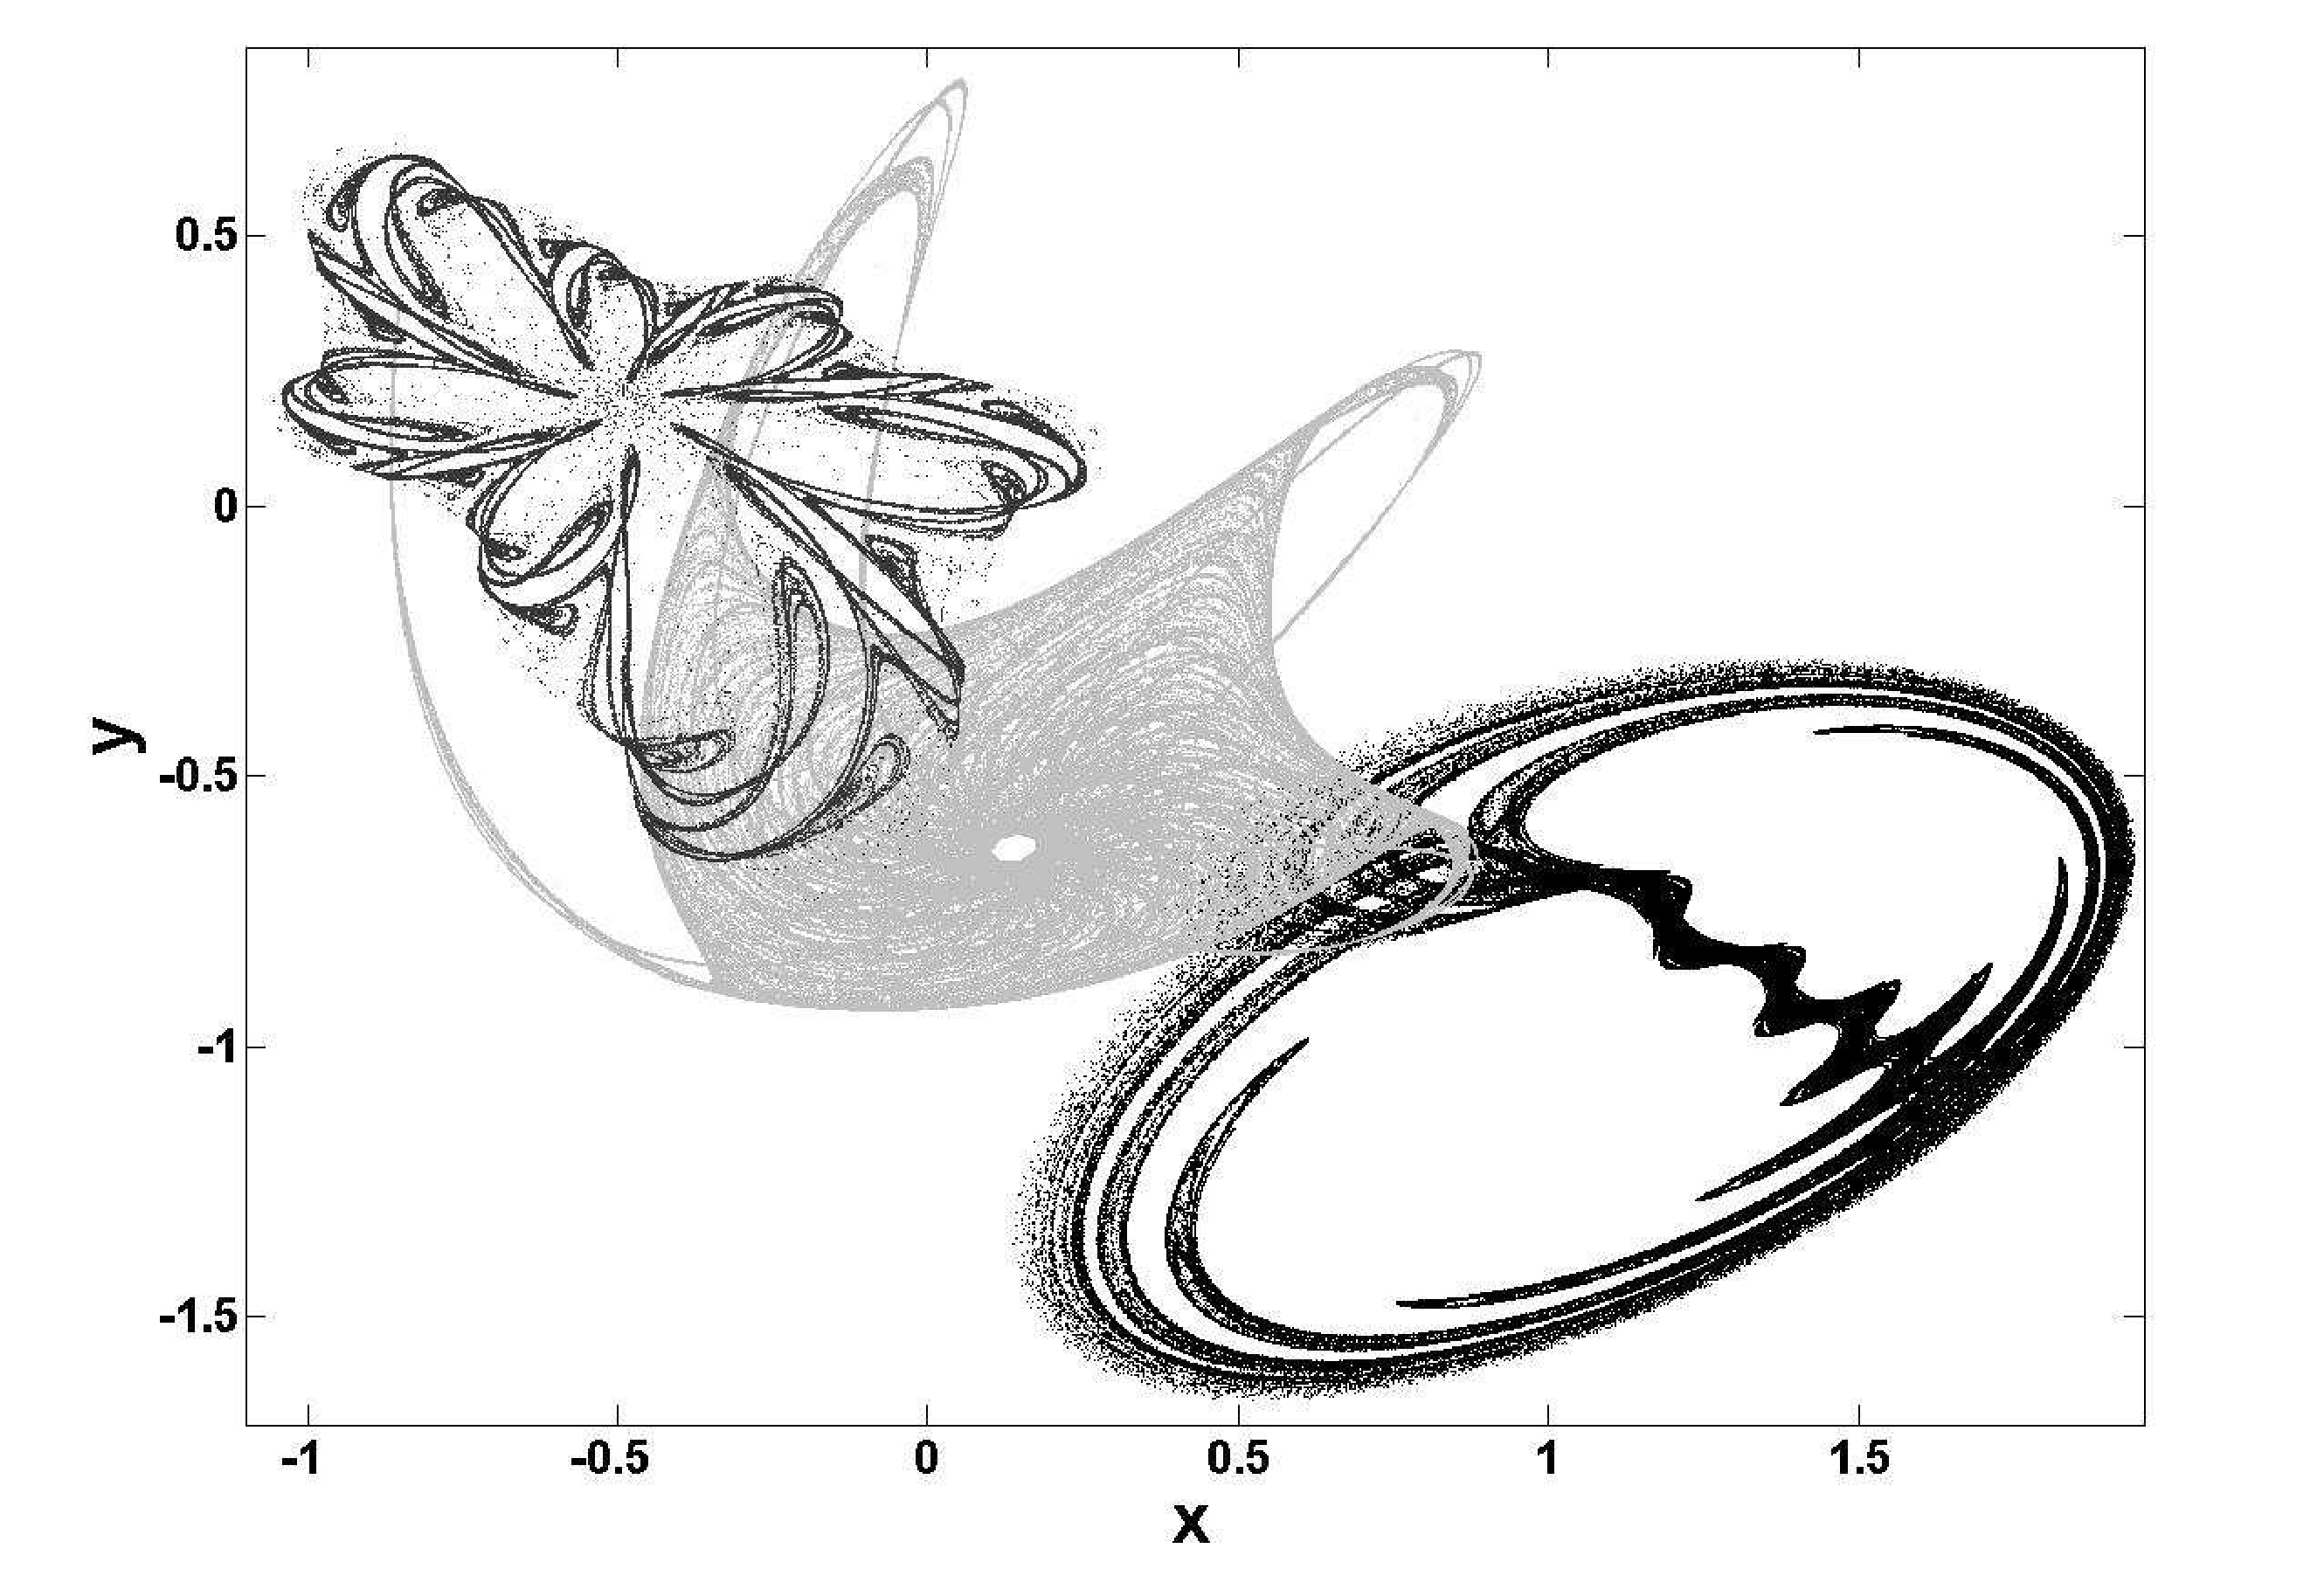
\includegraphics[width=1\columnwidth]{atractoreslindos}\\
    \caption{Three attractors for three different sets of  coefficients of $2D$-quadratic map.}\label{fig:atractores}
\end{figure}
%===========================================================================================
%
%==========================ATRACTORES 3, 5, 8 Y 2 CON SUS DOMINIOS============================
\begin{figure}
\begin{tabular}{cc}
\includegraphics[width=0.5\textwidth]{Atractor3_condominio_ok}
\includegraphics[width=0.5\textwidth]{Atractor5_condominio_ok}\\
\includegraphics[width=0.5\textwidth]{Atractor9_condominio_ok}
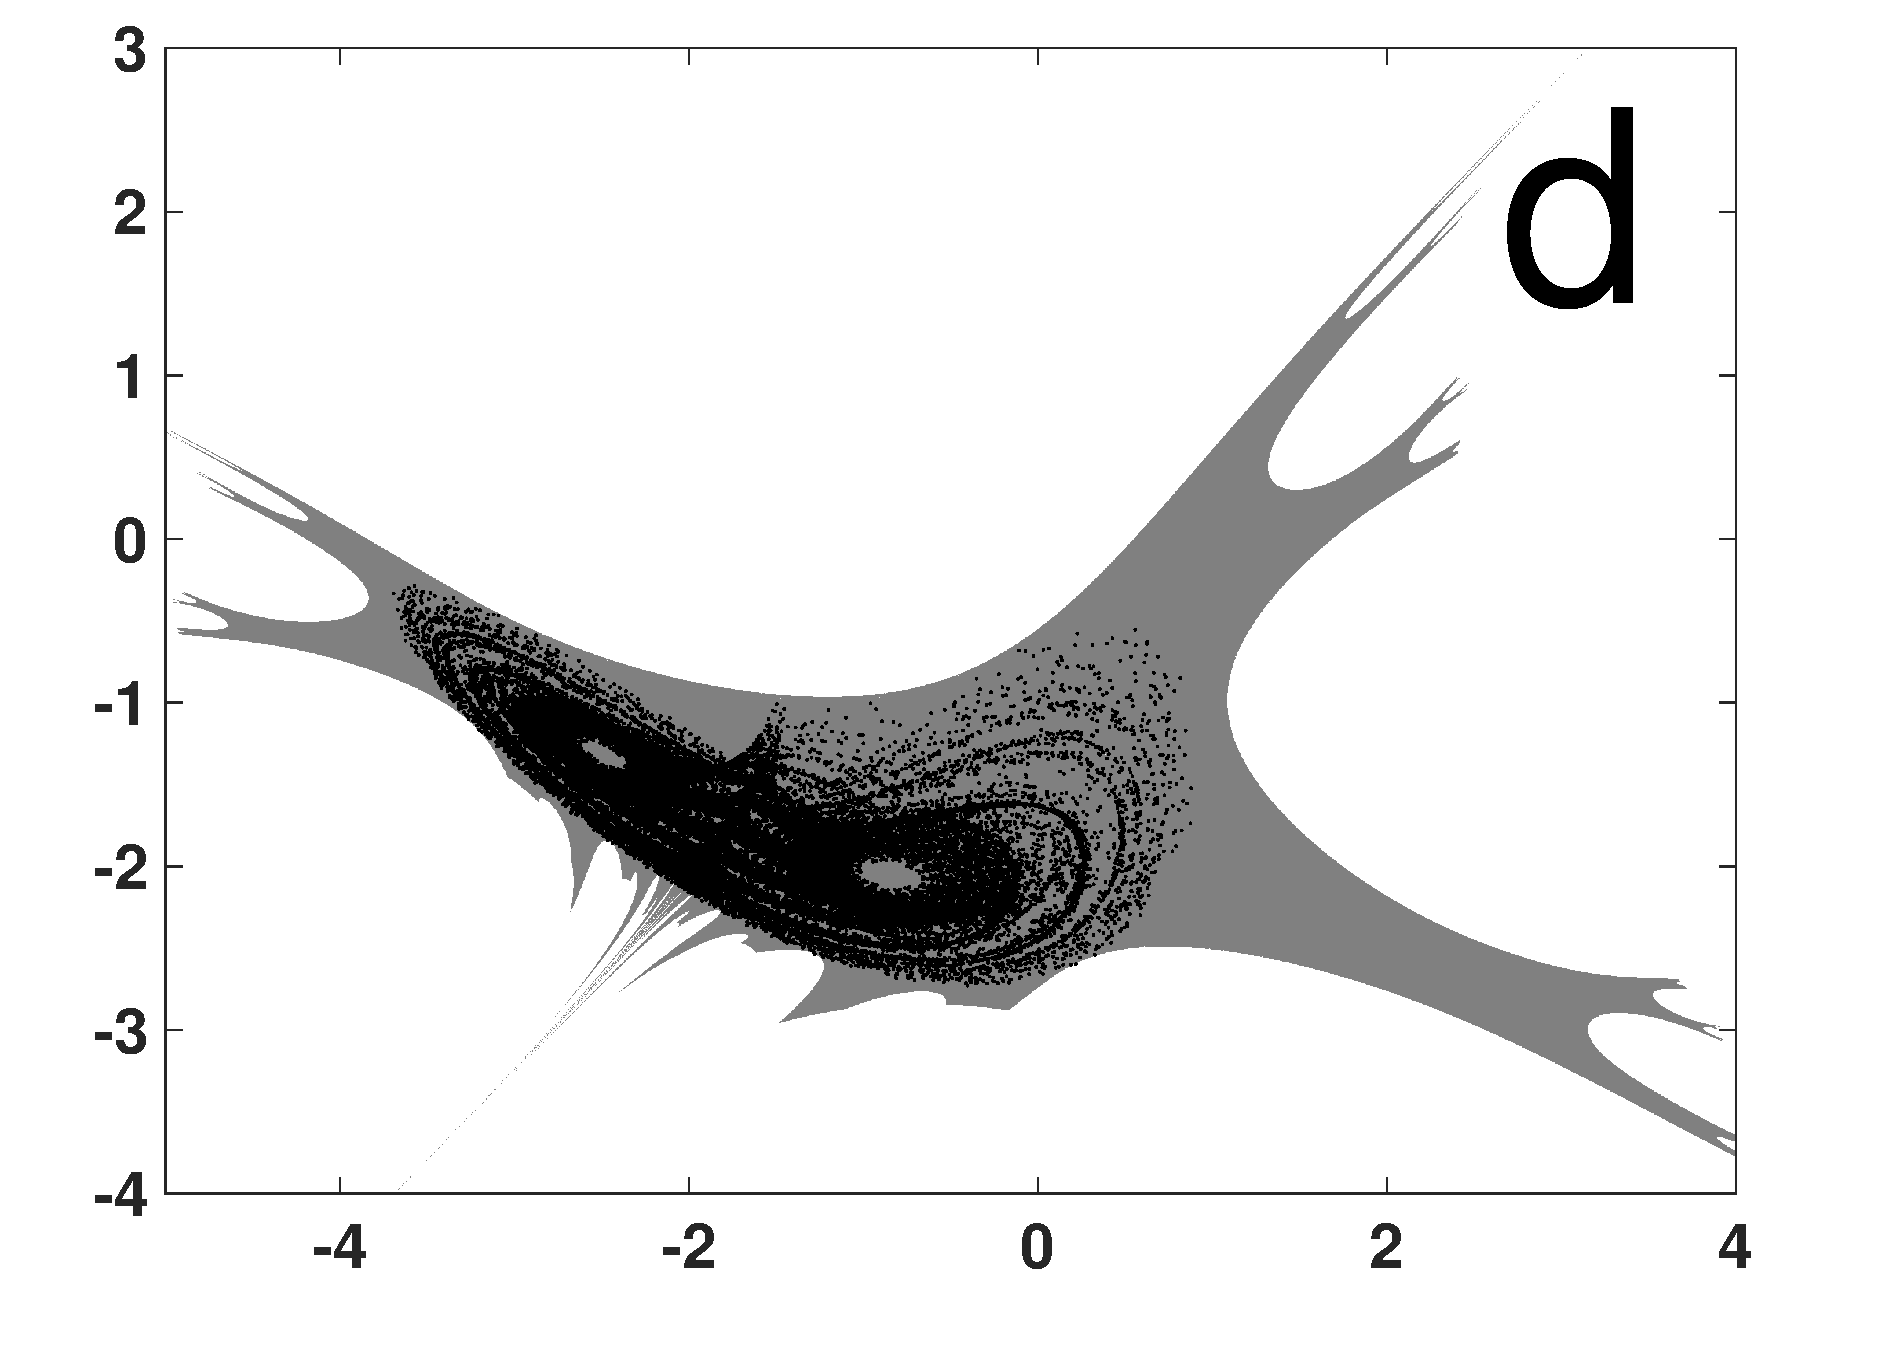
\includegraphics[width=0.5\textwidth]{Atractor2_condominio_ok}
\end{tabular}
\caption{Four chaotic attractors and their domains of attraction in floating-point arithmetics. The set of parameters are (see text):
(a) $\{a_i\}=A_1$; (b)  $\{a_i\}=A_2$; (c)  $\{a_i\}=A_3$;  (d) $\{a_i\}=A_4$, \cite{Sprott1993}.}
\label{fig:atractores3592}
\end{figure}

\section{Analysis tools}
\label{sec:quanti}

The normalized Shannon entropy applied to two different PDFs and the maximum Lyapunov exponent along with the mean period's lengths are the quantifiers employed here to estimate the system's properties. The entropies   help us to evaluate the two properties that determine the randomness degree, the equiprobability among all possible values and the statistical independence between consecutive values, while the MLE determines the presence of chaos. 
 
\subsection{Period analysis}

As said in section \ref{sec:estudio}, the maximum reachable period is $T_{max}=2^{d.n}$. Actually, the periods obtained are much lower than the maximum and are heavily dependent on the IC.

We have developed a C code that emulates the operation in a digital environment, it will be described in detail in section \ref{sec:repre}. One task of this code is to analyze the reached period when starting iteration from each initial condition with a certain number of bits. The initial condition could converge to a limit cycle, or it could be one value of the limit cycle itself. Basically, the code iterates every IC and detects when any value of the generated sequence is repeated, then it stores the period the limit cycle has.
This procedure was repeated for all the initial
conditions to obtain the attraction domain scheme of the
system.


With the developed code, we have systematically studied the behavior of the system's output
using different precisions in a fixed-point architecture.
\subsection{Quantifiers of Randomness}
\label{cu_ran}

Another important characteristic that varies with the precision employed is the randomness of the sequences generated by the chaotic system. 

Based on results of previous research \cite{DeMicco2008,Antonelli2016,DeMicco2011} the normalized Shannon entropy was adopted as quantifier to characterize determinism and stochasticity of the generated sequences. This quantifier derives from the Information Theory, and it is a functional of the PDF. Regarding the PDF, the classical probability distribution takes only into account the occurrence of values, but it is not able to detect the order of appearance of them. For example, a sequence of random values generated by any noise generator will exhibit a constant probability distribution between $0$ and $1$. On the other hand, a saw-tooth sequence will also present a constant probability distribution between $0$ and $1$. Because in both cases, the values appear in the series the same times but in a different order. This characteristic is crucial because it differences a random signal from an entirely predictable one. 
 
By a proper selection of the used PDF it is possible to cover the two mentioned properties, namely, (1) the probability of occurrence of each element of the alphabet (PDF based on histograms), and (2) the order of the items in the time series (PDF based on Bandt-Pompe technique).
A discussion about the convenience of using these quantifiers is beyond the scope of this chapter but there is an extensive literature \cite{Rosso2007A,DeMicco2008,Martin2006}.

Once the PDF is determined the entropy is defined by the very well known normalized Shannon expression:

\begin{equation}
H=\frac{\sum_{i=1}^{M}{p_i~log~p_i}}{log(M)}, \label{eq:shannon}
\end{equation}

Where $M$ is the number of elements of the alphabet.
\subsubsection{Defining the PDF:}

From a statistics point of view a chaotic system is the \textsl{source} of a symbolic time series with an alphabet of $M$ symbols. Entropy is a basic concept in information theory. To evaluate entropy  one needs first to define a probability distribution function of the time series. There is not a unique procedure to obtain this PDF and the determination of the best PDF $P$ is a fundamental problem because $P$ and the sample space are inextricably linked.
Several methods deserve mention: 
\begin{enumerate}
\item frequency counting \cite{Rosso2009}, 
\item procedures based on amplitude statistics \cite{DeMicco2008}, 
\item binary symbolic dynamics \cite{Mischaikow1999}, 
\item Fourier analysis \cite{Powell1979}, 
\item wavelet transform \cite{Rosso2001} and,
\item ordering patterns \cite{Pompe2002}, among others.  
\end{enumerate}
Their applicability depends on particular characteristics of the data, such as stationarity, time series length, variation of the parameters, level of noise contamination, etc.

Basically one may consider the statistics of individual symbols or the statistics of sequences of $D$ consecutive symbols. In the first case  $P$ is \emph{non-causal} because it does not change if the outcomes are mixed up and the number of different possible outcomes is $M$ (the number of symbols in the source alphabet). In the second case, the outcome changes if the output is mixed and then one says that $P$ is \emph{causal}. In this second case the number of different outcomes is equal to $M^D$ and increases rapidly with $D$. Bandt and Pompe made a proposal in \cite{Pompe2002} that is computationally efficient, because it limits the outcomes to $D!$, but retains causal effects. In previous works devoted to PRNGs, the use of two
PDFs was successful for the comparison between different systems. One PDF is the
normalized histogram, and its normalized Shannon
entropy is denoted here $H_{hist}$. The other one is the ordering PDF
proposed by Bandt \& Pompe \cite{Pompe2002} and its  normalized Shannon entropy is  here denoted as $H_{BP}$. Let us summarize how these
PDFs are obtained.

The representation plane $H_{BP}$ vs $H_{hist}$ is considered \cite{DeMicco2008}.
A higher value in any of the entropies, $H_{BP}$ and $H_{hist}$, implies an
increase in the uniformity of the involved PDFs. The point
$(1,1)$ represents the ideal point for a system with uniform histogram and
uniform distribution of ordering patterns.
\subsubsection{PDF based on histograms}

To evaluate the probability of occurrence of each element of the alphabet, it is possible to use the normalized histogram of the time series as a PDF.

If $Y$ is the time series being analysed $Y=\{y_i,i=1,...N\}$. The obvious PDF to characterize $Y$ is the normalized histogram of the $M$ words $Y$; let us call it  $PDF_{hist}$.
 
In order to  extract a PDF via amplitude-statistics, divide first
the interval $[0,1]$ into a finite number $nbin$ of non
overlapping subintervals $A_i$: $[0,1]=\bigcup_{i=1}^{nbin} A_i$
and $A_i\bigcap A_j=\emptyset~\forall i\neq j$. One then employs
the usual histogram-method, based on counting the relative
frequencies of the time series values within each subinterval. It
should be clear that the resulting  PDF lacks any information
regarding temporal evolution. The only pieces of information we
have here are the $y_i$-values that allow one to assign inclusion
within a given bin, ignoring just where they are located (this is,
the subindex $i$.)

\subsubsection{PDF based on Band and Pompe methodology}
%
Let $y$ be the source output and let $y_1$ to $y_N$ be a $N$-length digital time series.
To use the Bandt and Pompe \cite{Pompe2002} methodology for evaluating
of probability distribution $P$ one starts by  considering
a vector of length $D$ given by: 
\begin{equation}
(s)~\mapsto~
\left(~y_{s-(D-1)},~y_{s-(D-2)},~\dots,~y_{s-1},~y_{s}~\right) \,
 \label{eq:vectores}
\end{equation}

which assign to each time $s$ the $D$-dimensional vector of values
at times $s, s-1,\dots,s-(D-1)$. Clearly, the greater the
$D$-value, the more information on the past  is incorporated into
our vectors. By the ``ordinal pattern" related to the time $(s)$
we mean the permutation $\pi=(r_0,r_1, \dots,r_{D-1})$ of
$(0,1,\dots,D-1)$ defined by
\begin{equation}
y_{s-r_{D-1}}~\le~y_{s-r_{D-2}}~\le~\dots~\le~y_{s-r_{1}}~\le~y_{s-r_0}
\ . \label{eq:permuta}
\end{equation}
In order to get a unique result we set $r_i <r_{i-1}$ if
$y_{s-r_{i}}=y_{s-r_{i-1}}$. Thus, for all the $D!$ possible
permutations $\pi$ of order $D$, the probability distribution
$P=\{p(\pi)\}$ is defined by
\begin{equation}
p(\pi)~=~\frac{\# \{s|s\leq N-D+1;~ (s) \texttt{, has type
}\pi\}}{N-D+1} \ . \label{eq:frequ}
\end{equation}
In this expression, the symbol $\#$ stands for ``number".

The Bandt-Pompe's methodology is not restricted to time series
representative of low dimensional dynamical systems but can be
applied to any type of time series (regular, chaotic, noisy, or
reality based), with a very weak stationary assumption (for $k =
D$, the probability for $y_t < y_{t+k}$ should not depend on $t$
\cite{Pompe2002}). One also assumes that enough data are available for
a correct attractor-reconstruction. Of course, the embedding
dimension $D$ plays an important role in the evaluation of the
appropriate probability distribution because $D$ determines the
number of accessible states $D!$. Also, it conditions the minimum
acceptable length $N \gg D!$ of the time series that one needs in
order to work with a reliable statistics.


\subsection{Maximum Lyapunov Exponent}

The fourth quantifier employed is the Maximum Lyapunov Exponent that determines the presence of chaos.
The Lyapunov exponents are quantifiers that characterize how the
separation between two trajectories evolves, \cite{Sprott2003}. It
is well known that chaotic behaviors are characterized
mainly by Lyapunov numbers of the dynamic systems. If one or more
Lyapunov numbers are greater than zero, then the system behaves
chaotically. Otherwise, the system is stable. In this paper, we
employ the maximum Lyapunov number as it is one of the most useful
indicators of chaos.

The distance between trajectories changes in $2^{MLE}$ for each
iteration, on average. If $MLE<0$ the trajectories approaches,
this may be due to a fixed-point, if $MLE=0$ the trajectories keep
their distance, this may be due to a limit cycle, if $MLE>0$, the
distance between trajectories is growing, and is an indicator of
chaos, \cite{Sprott2003}.

There is a non-analytical way to measure it if only the inputs and
outputs of the system are accessible. The procedure is the
following: the system must be started from two neighbor points in
the phase plane, lets call them $(x_a,y_a)$ and $(x_b,y_b)$, as
the system is iterated the Euclidean distance between the two
trajectories is measured ($d_n$ in the $n_{th}$ sample) (eq.
\ref{eq:D0D1}), and the b trajectory is relocalized on each
iteration  (eq. \ref{eq:reubicacion}), obtaining the points
$(x_{br},y_{br})$ to feed the system. Then the Lyapunov exponent
can be calculated as shown in eq. (\ref{eq:Lyapunov}).

\begin{eqnarray}\label{eq:Lyapunov}
    MLE &=& \frac{1}{N} \sum_{i=2}^{N} \log_2{\frac{d_{1(i)}}{d_{0(i-1)}}}
\end{eqnarray}
\begin{eqnarray}\label{eq:D0D1}
    d_{0(i-1)}&=& \sqrt{(x_{a(i-1)}-x_{br(i-1)})^2+(y_{a(i-1)}-y_{br(i-1)})^2}\nonumber\\
    d_{1(i)}&=& \sqrt{(x_{a(i)}-x_{b(i)})^2+(y_{a(i)}-y_{b(i)})^2}\\
\nonumber
\end{eqnarray}
\begin{eqnarray}\label{eq:reubicacion}
    x_{br(i)}&=& x_{a(i)}+(x_{b(i)}-x_{a(i)})d_{o(i-1)}/d_{1(i)} \nonumber\\
    y_{br(i)}&=& y_{a(i)}+(y_{b(i)}-y_{a(i)})d_{o(i-1)}/d_{1(i)}
\end{eqnarray}




\section{Hardware Digital Simulation.} \label{sec:repre}
%\section{Degradation of the domains of attraction for fixed point arithmetics}

Within the available options for representing values using finite precision, floating-point arithmetic is the closest to $\mathbb{R}$. However, from the engineering point of view the usage of floating-point is not efficient when compared to fixed-point operations because the first ones consume lot of system resources and require several clock cycles. It is widely known that when the maximal values to be represented and the precision required are pre-established fixed-point arithmetic would allow getting better results in terms of velocity, usage resources and power consumption.

The analysis in this paper was intended to cover any digital electronic device such as FPGA, CPLD (Complex Programmable Logic Device) or ASIC (Application Specific Integrated Circuit). On this kind of devices, saving resources is a crucial issue, this is why they mostly employ fixed-point arithmetic. 

A C code that simulates iterating a nonlinear system, the quadratic map, in any of such devices was developed in order to generate sequences which were then analyzed.
The code is totally parametrizable and it allows to access intermediate values.
A technique that emulates operating in fixed-point arithmetic was employed, the general idea is to use signed integer arithmetic, although chaotic systems work with fractional numbers. To solve this, an equivalence
between fractional fixed-point numbers and signed integers was employed here.

Of course, internally all digital device works with binary numbers, designers interpret these bits based on the architecture they want to work with. 
Binary numbers can be interpreted as integer numbers or, as in this case, they can be thought in terms of a fractional point located at a certain position. To illustrate this:

\begin{equation}\label{eq:eqdecimal}
Fractional\_fixed\_point=-b_{n_i-1}.2^{(n_i-1)} \dots b_0.2^0,b_{-1}.2^{-1} \dots b_{-n_f}2^{-n_f}
\end{equation}

where we called $n_i$ to the number of bits used to represent the integer part and $n_f$ the fractional, the whole number of bits is $n=n_i+n_f$.

In order to make this conversion, each fractional number must be
multiplied by $2^{n_f}$ to obtain its equivalent Signed Integer
number. Where $n_f$ is the quantity of bits used to represent the
fractional part of the number. This is equivalent to right-shift $n_f$
positions the fractional point. Resulting in:

\begin{equation}\label{eq:eqentero}
Signed\_integer= -b_{n_i-1+n_f}.2^{(n_i-1+n_f)} \dots b_0.2^0
\end{equation}

An example of the equivalence is shown in Table \ref{tab:tabla}. This Table shows the equivalence when
using $n=6$ bits, $2$ bits for the integer part and $4$ bits
for the fractional part ($n_i=2$ and  $n_f=4$).
The following considerations must be taken into account when operating with this equivalence:

\begin{itemize}
    \item Addition, this operation does not need any consideration just to make sure not to exceed the limits of the arithmetic used.
    \item Multiplication, the result of this operation must be divided by $2^{n_f}$ to adjust the result to the correct range.
    \item Division, the result must always be rounded towards minus infinity. This is, $7.28$ to $7$ , $-14.9$ to $-15$.
\end{itemize}

After each operation, the corresponding adjustment is performed to operate identically as digital devices work.

For generating data, the system was intended to be working in fractional fixed-point
architecture with $4$ bits for representing the integer
part, $n_i=4$, in two's complement representation ($Ca_2$). The code automatically varies the
number of bits representing the fractional part of the number, $n_f$,
in order to analyze how the system reacts when the precision
changes.


\begin{table}[h]
  \caption{Example of equivalences.}\label{tab:tabla}
  \vspace{2mm}
  \centering
  \begin{tabular}{ c c c  }
  \hline
  Binary  & Fractional Fixed point & Signed Integer  \\
  \hline
   \hline
  $01.1111$ & $1.9375$ & $31$ \\
  $01.1110$ & $1.8750$ & $30$ \\
  $01.1101$ & $1.8125$ & $29$ \\
   \vdots & \vdots &  \vdots\\
  $00.0000$ & $0.00$ & $0$  \\
  $11.1111$ & $-0.0625$ & $-1$ \\
  $11.1110$ & $-0.1250$ & $-2$  \\
   \vdots & \vdots & \vdots \\
    $10.0000$ &  $-2.00$ & $-32$  \\
    \hline
    \end{tabular}
\end{table}

The developed code iterates the $2D$-quadratic map $10^5$ times, in this case coefficients $a_0$ to $a_{11}$ have the values:\\
$\{a_i\}=\{-1.0, 0.9, 0.4, -0.2, -0.6, -0.5, 0.4, 0.7, 0.3, -0.5, 0.7,-0.8\}$. 

The map has been iterated with ICs $x_0$ and $y_0$, with $x_0$ and $y_0~\in~[-2,2]$. They have been swept in steps determined by the $n_f$ employed.
For example, when using five bits to represent the fractional part of the number ($n_f=5$), the minimum value (minimum grid) that can be represented is $0.0063$. In the case of using six bits the resulting minimum value is $0.0026$, in general when using $n_f$ bits the resulting step\_grid will be:

\begin{equation}
step\_grid=\frac{1}{n_f.2^{n_f}}
\end{equation}

On each case it was determined whether the
systems evolves to a fixed point, diverges or goes towards a
periodic cycle.

For every value of precision $n_f$ the code outputs a square matrix of order $4.n_f.2^{n_f}$ whose elements correspond to the final state of the system when initialized with each
IC. This means each position will contain one of three values:
\begin{itemize}
\item $-1$, if it diverged,
\item $0$, if it converged to a fixed point, 
\item the length of the period, at which that IC converged.
\end {itemize}

An interesting thing about this program is that it is independent of where it runs, and of the arithmetic used by it (float, double, long double, etc.).

For each detected cycle, with every $n_f$, a sequence of length $10^7$ was generated for calculating the randomness quantifiers previously introduced in section \ref{cu_ran}. 
From the point of view of a PRNG implementation and specifically encryption, the desirable properties for the system will be to present large periods with good statistical properties, few fixed
points of course, that do not diverge.

\section{Results} \label{sec:results}

Figure \ref{fig:avvelo} displays the obtained domains of attraction for $n_i=4$ and some values of $n_f$. The abscissa and ordinate axis correspond to initial values of $x$ and $y$ respectively. Each point represents an IC and the colour is associated to its final state,  the darker the tone of grey the shorter the cycle, fixed points are in black and divergent points in white. So, the different domain attractors (including the attractors) that coexist in the system can be seen here.



\begin{figure}
  \centering
\begin{tabular}{cc}
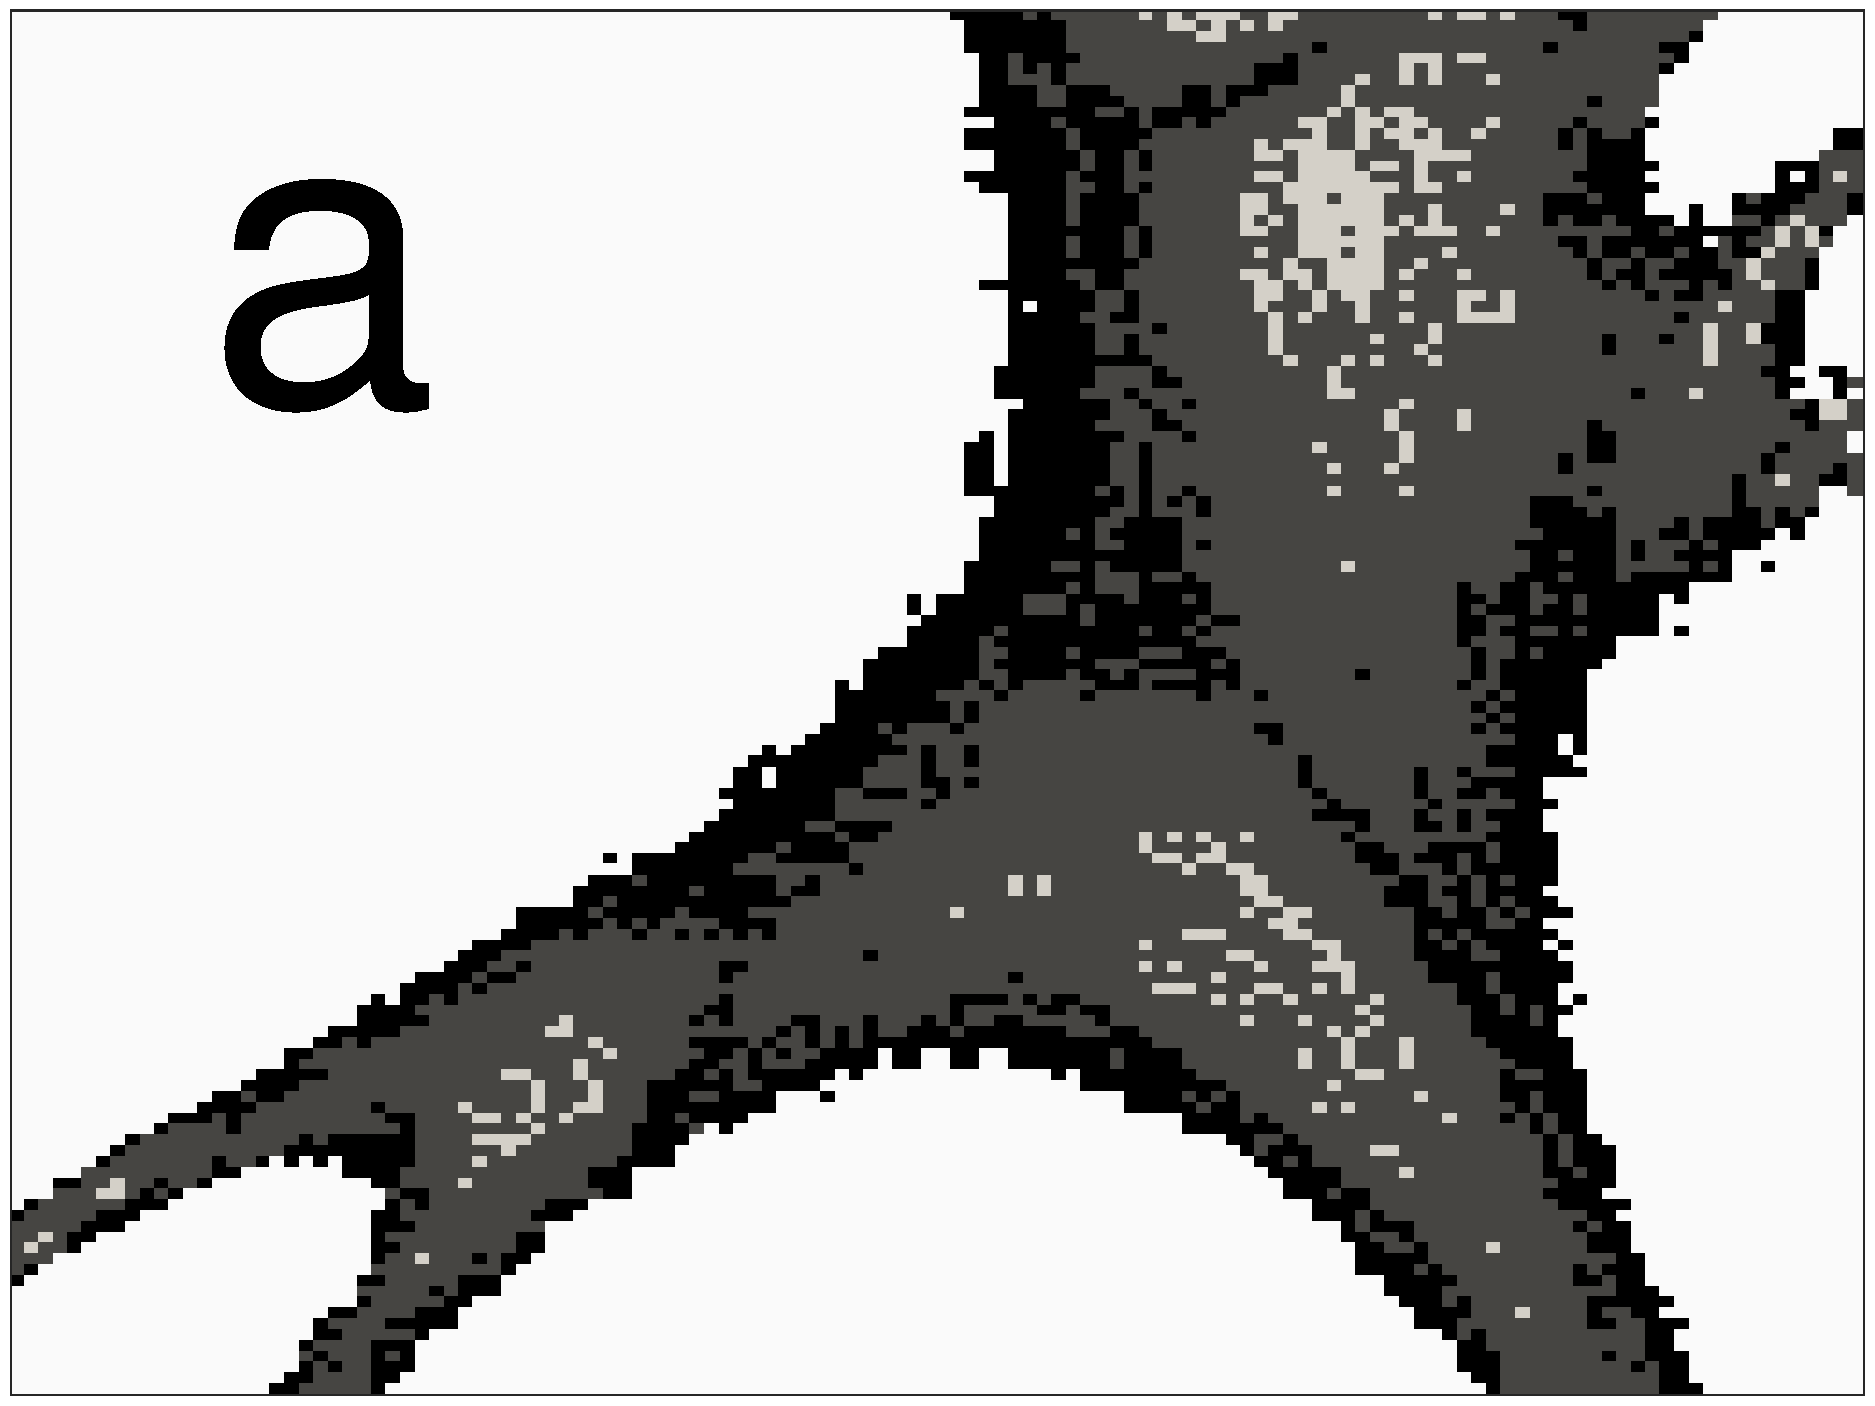
\includegraphics[width=0.3\textwidth]{m5_lu}
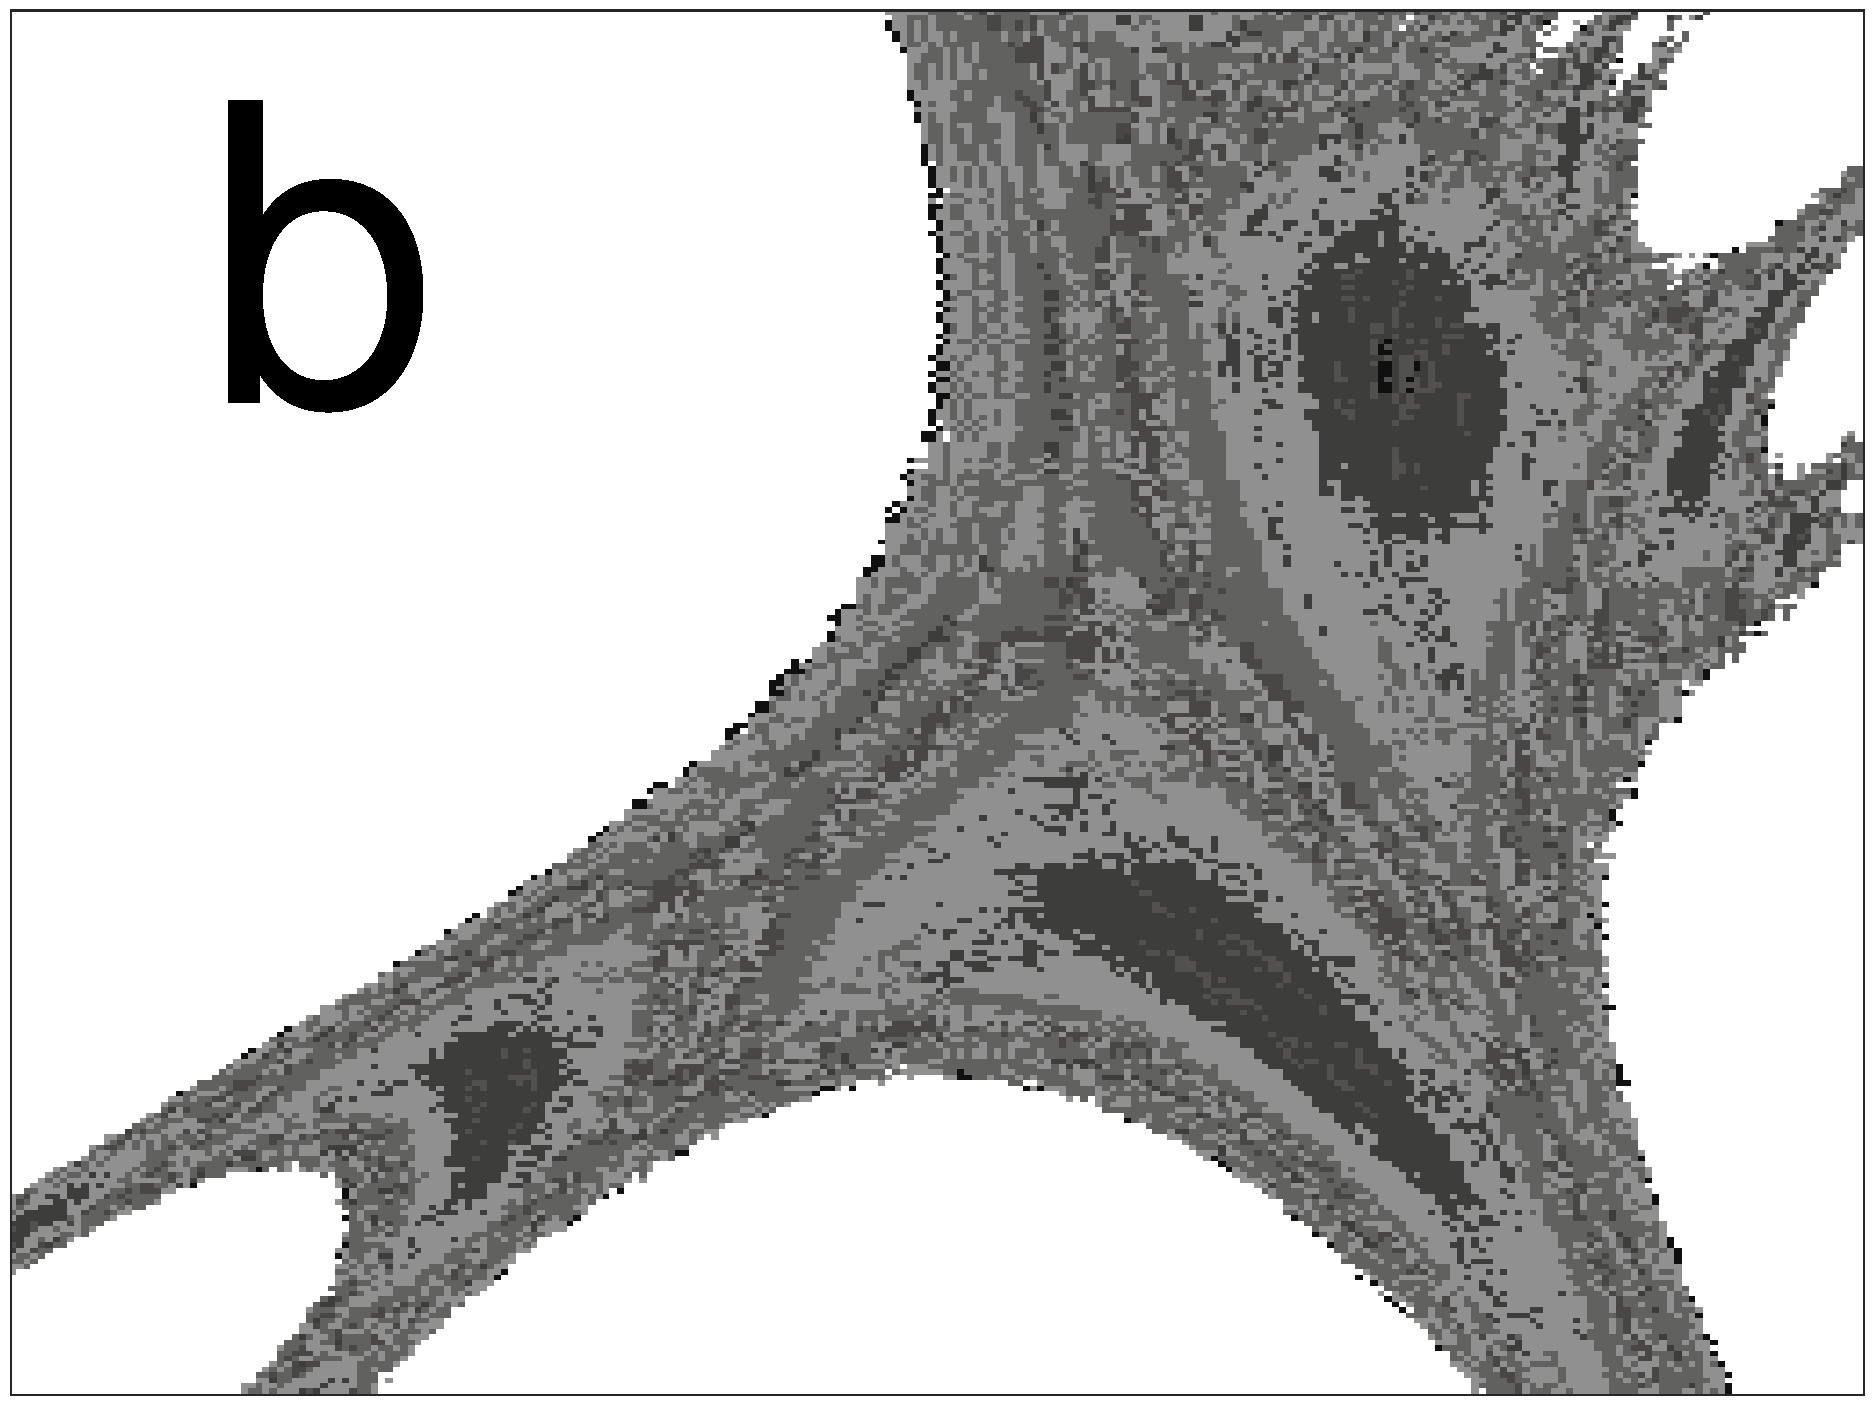
\includegraphics[width=0.3\textwidth]{m6_lu}
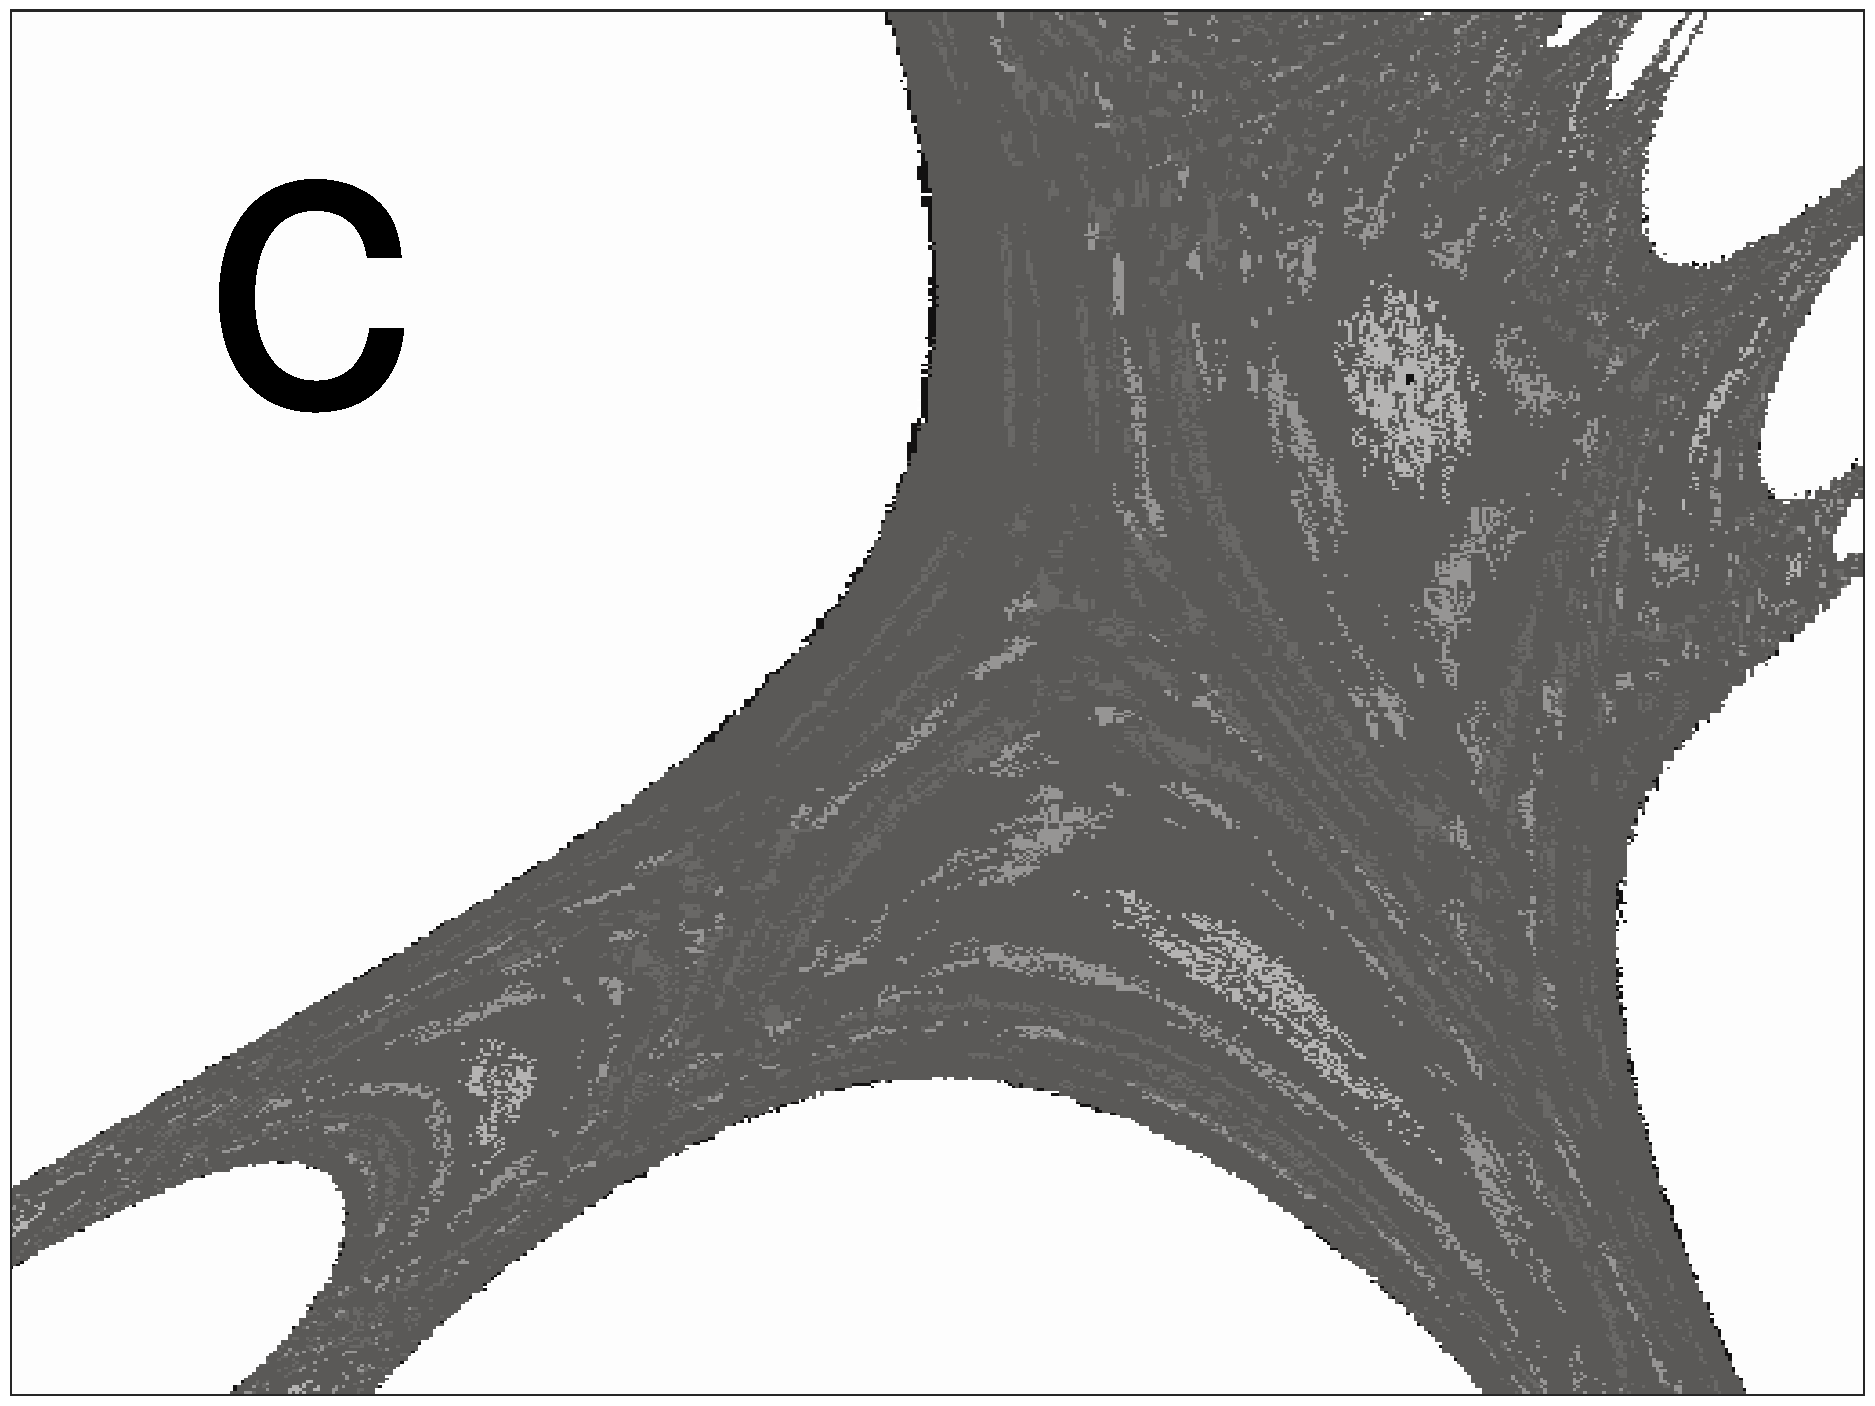
\includegraphics[width=0.3\textwidth]{m7_lu}\\
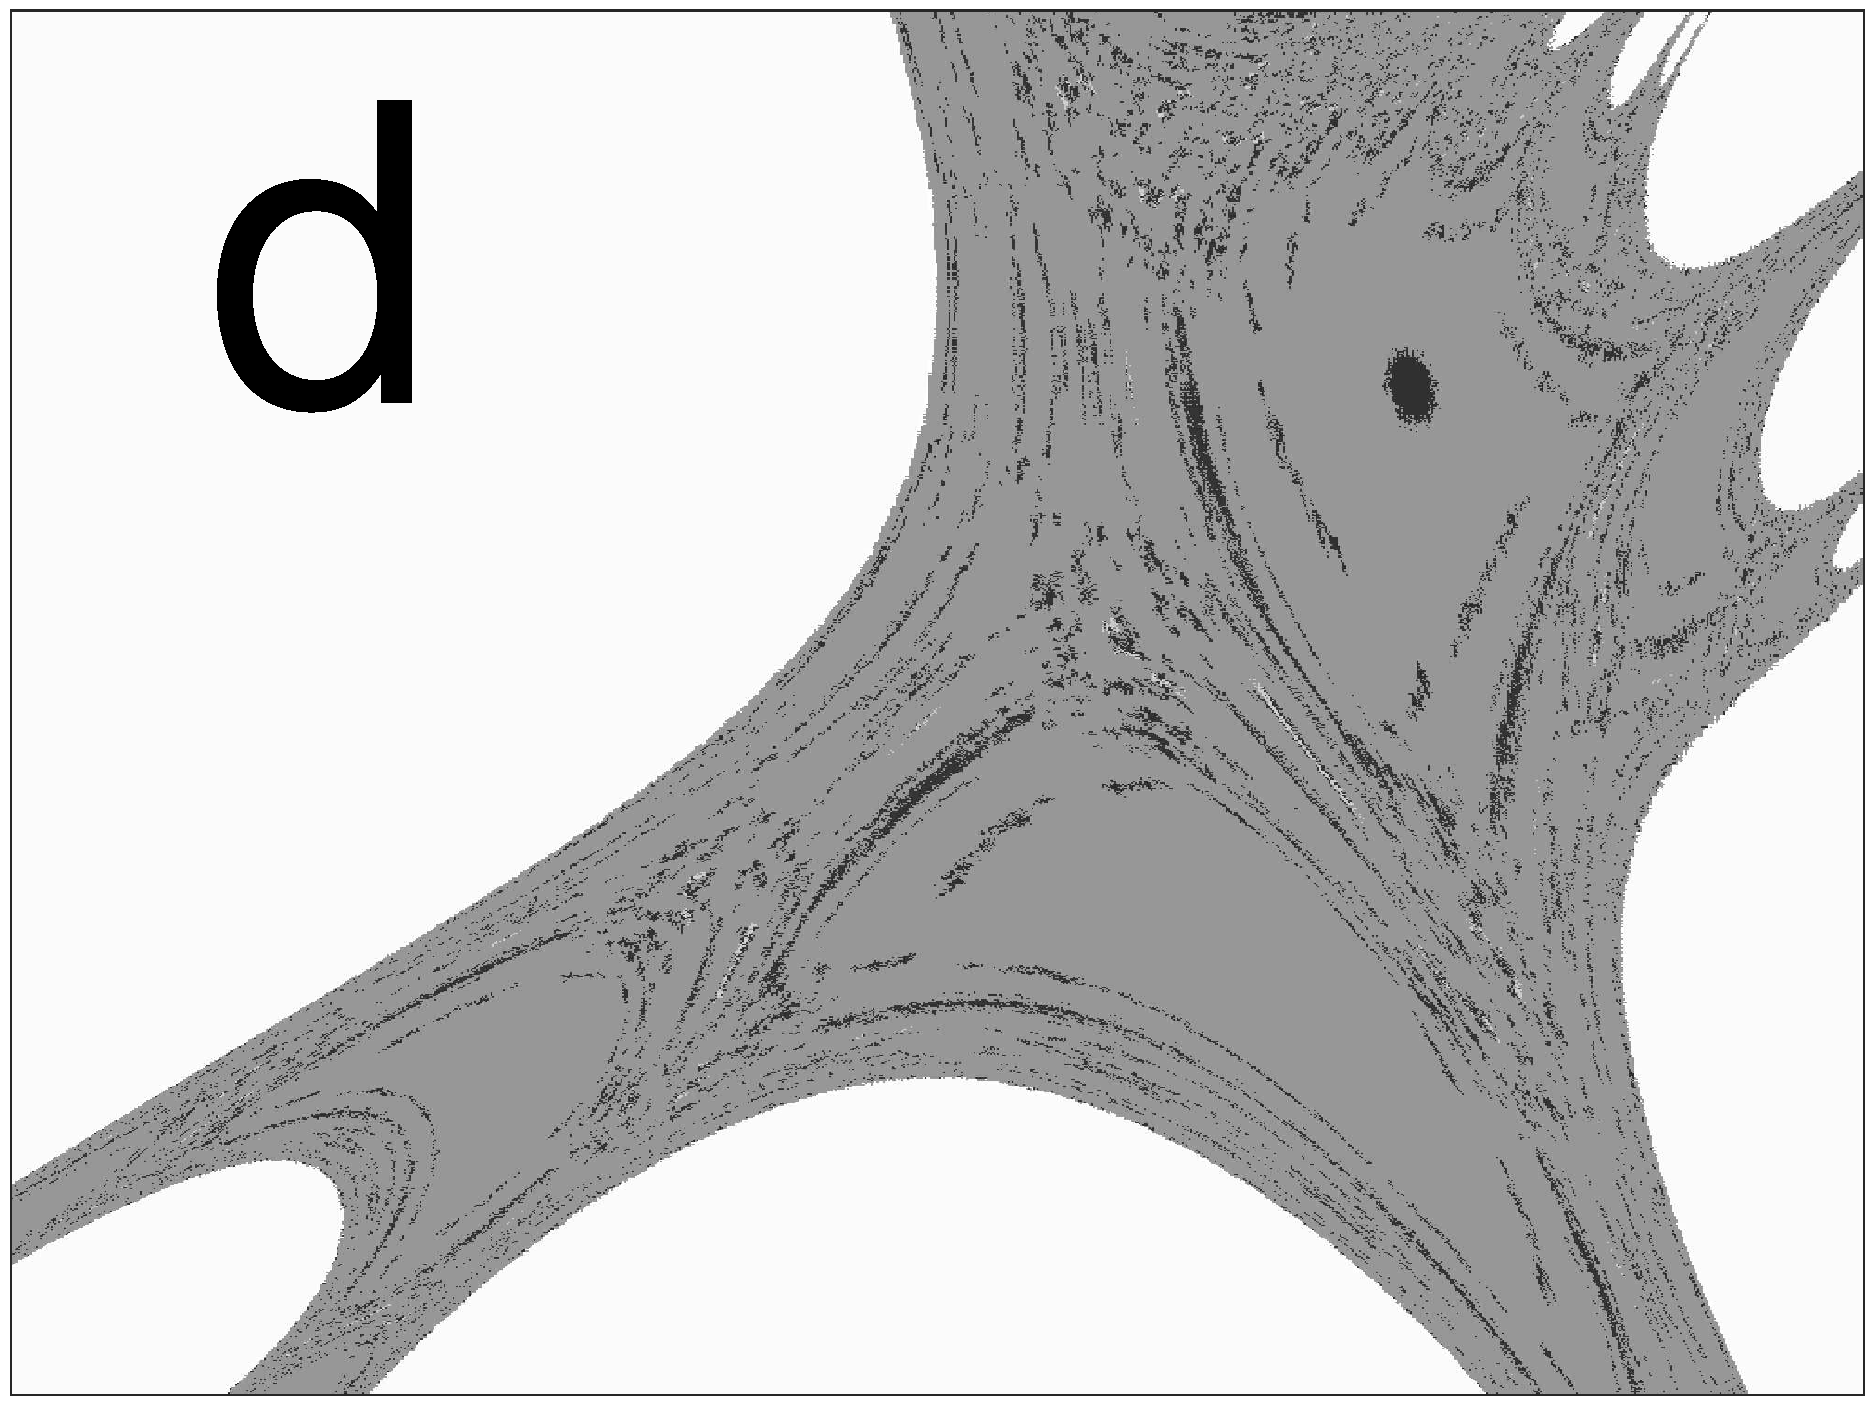
\includegraphics[width=0.3\textwidth]{m8_lu}
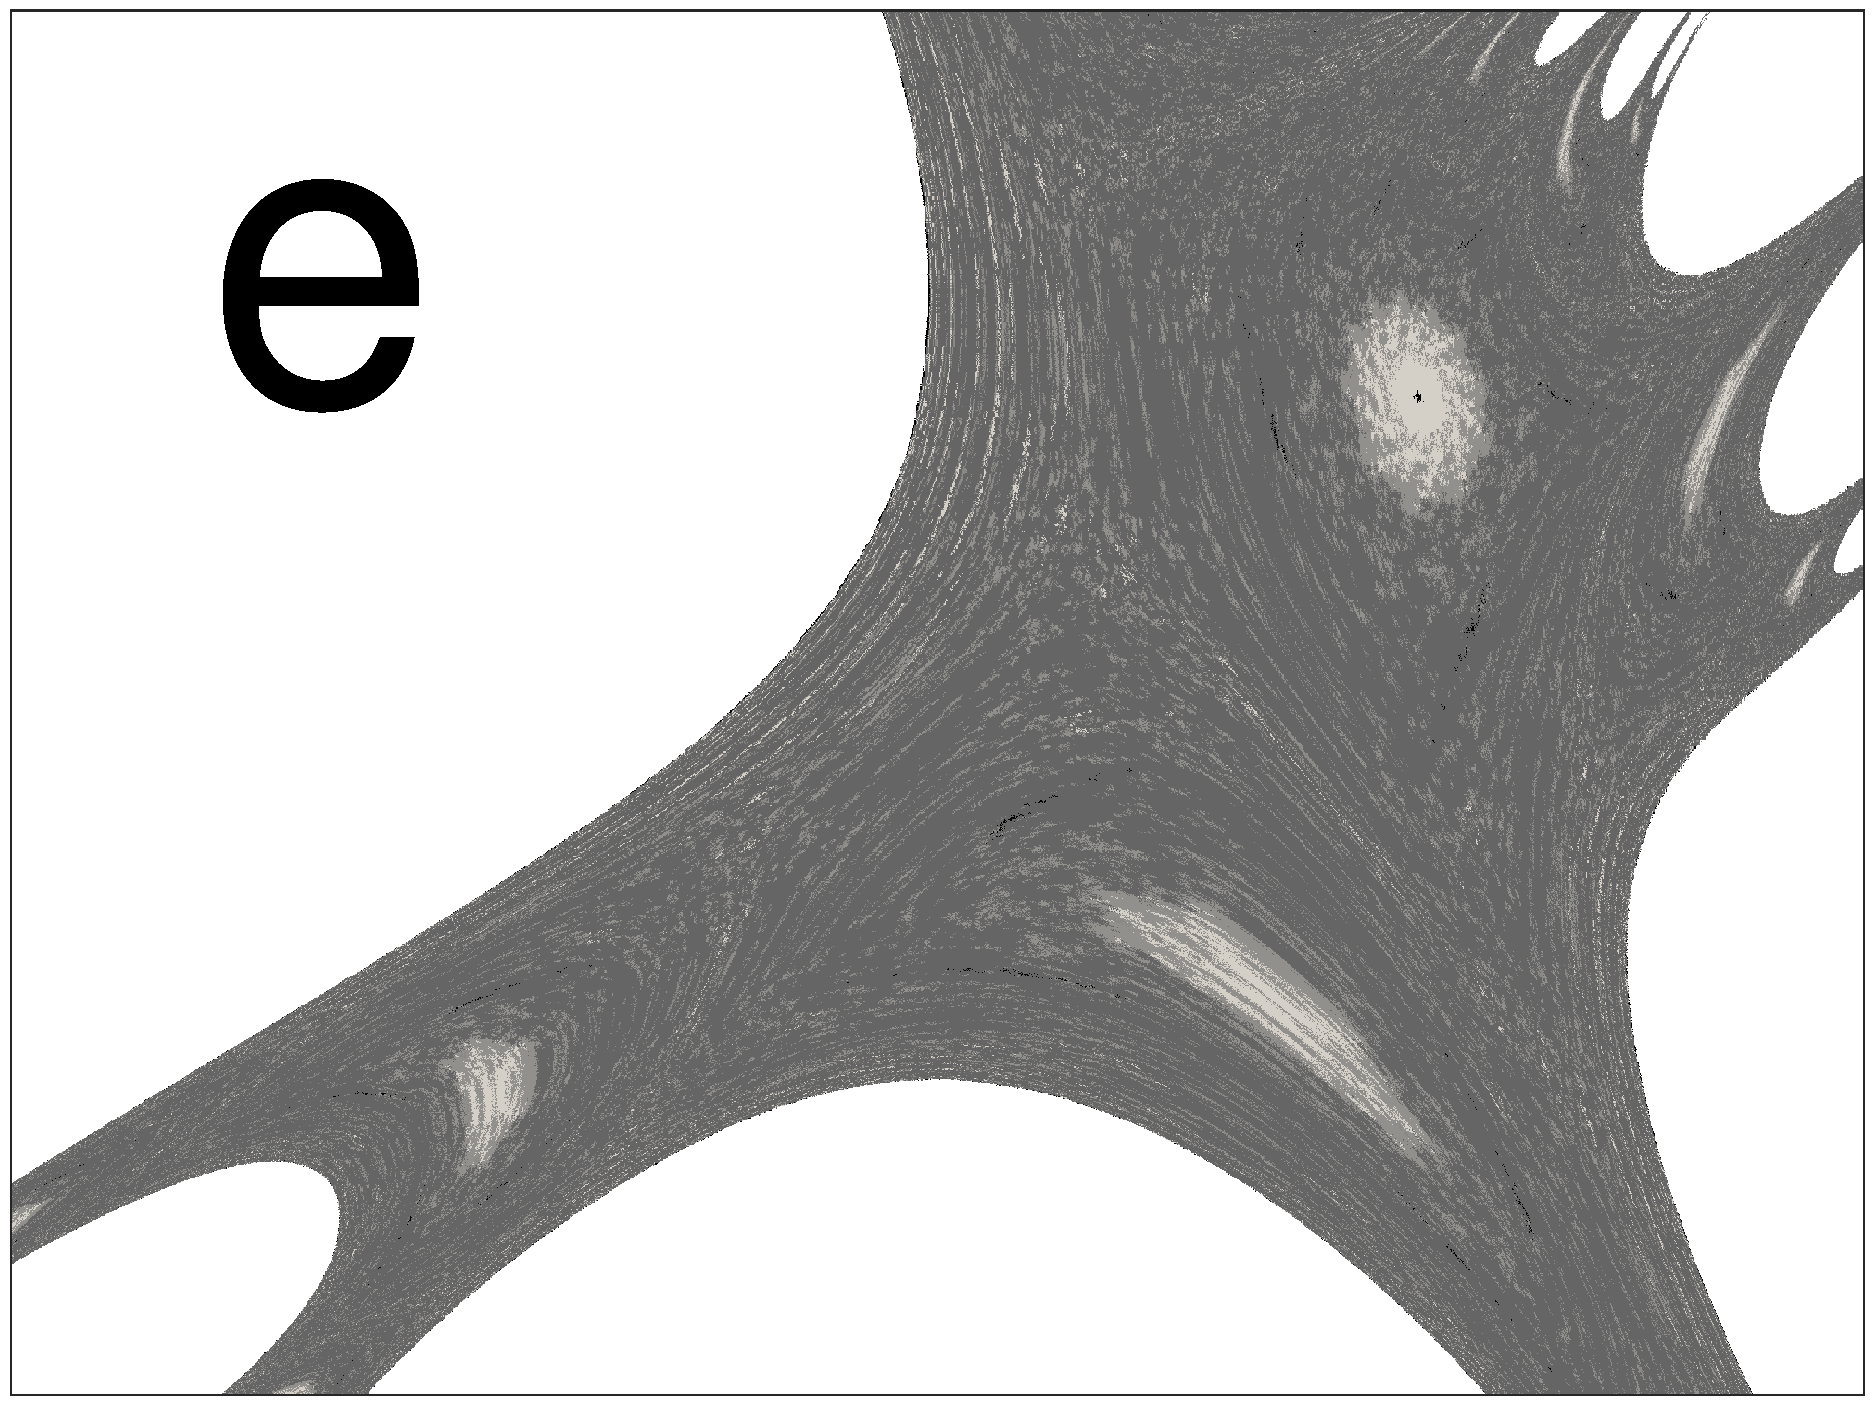
\includegraphics[width=0.3\textwidth]{m9_lu}
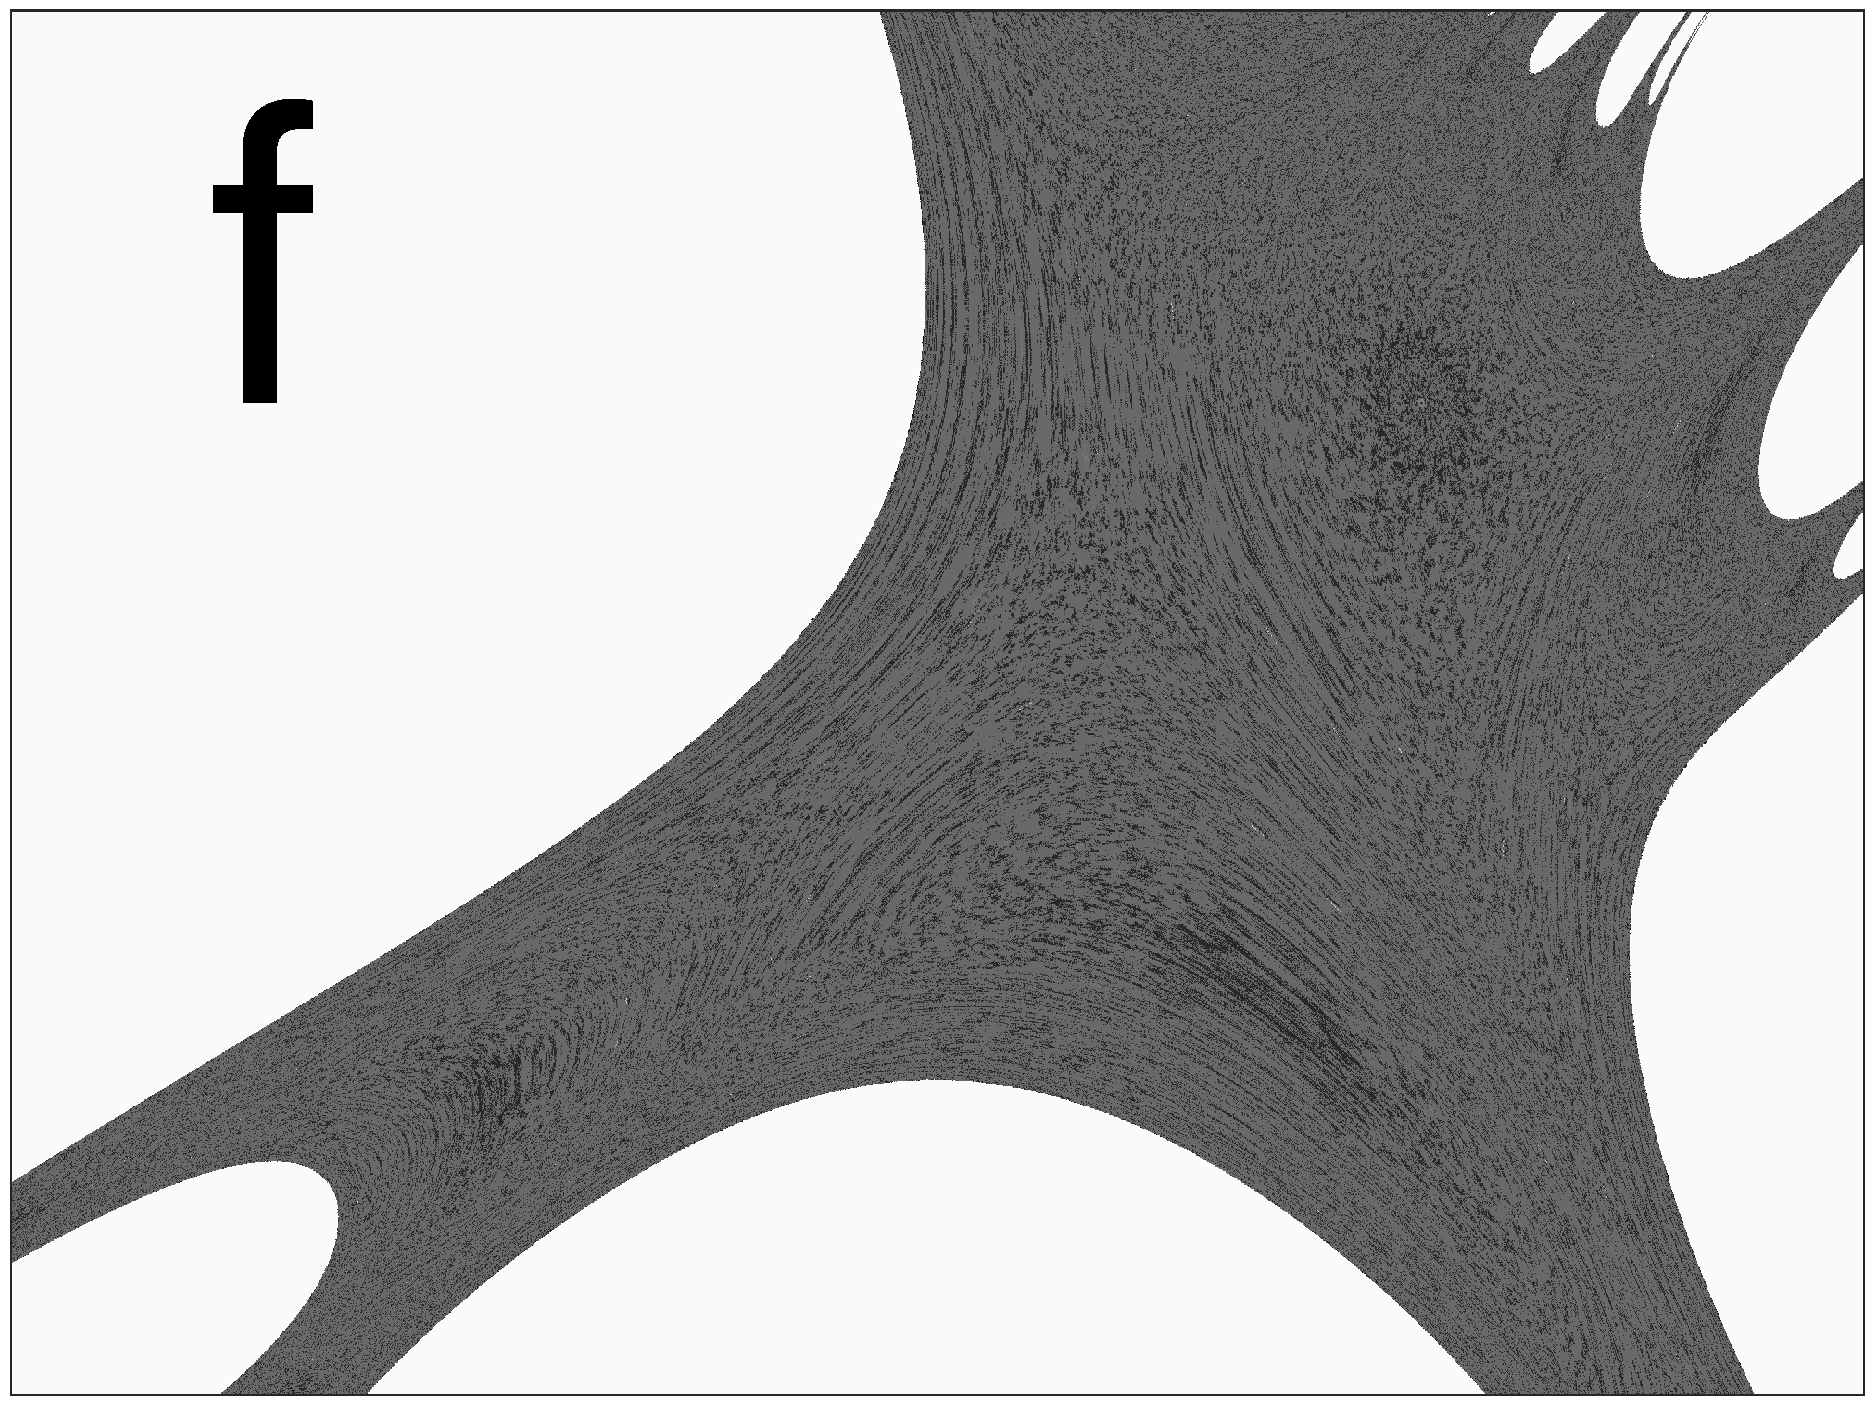
\includegraphics[width=0.3\textwidth]{m10_lu}\\
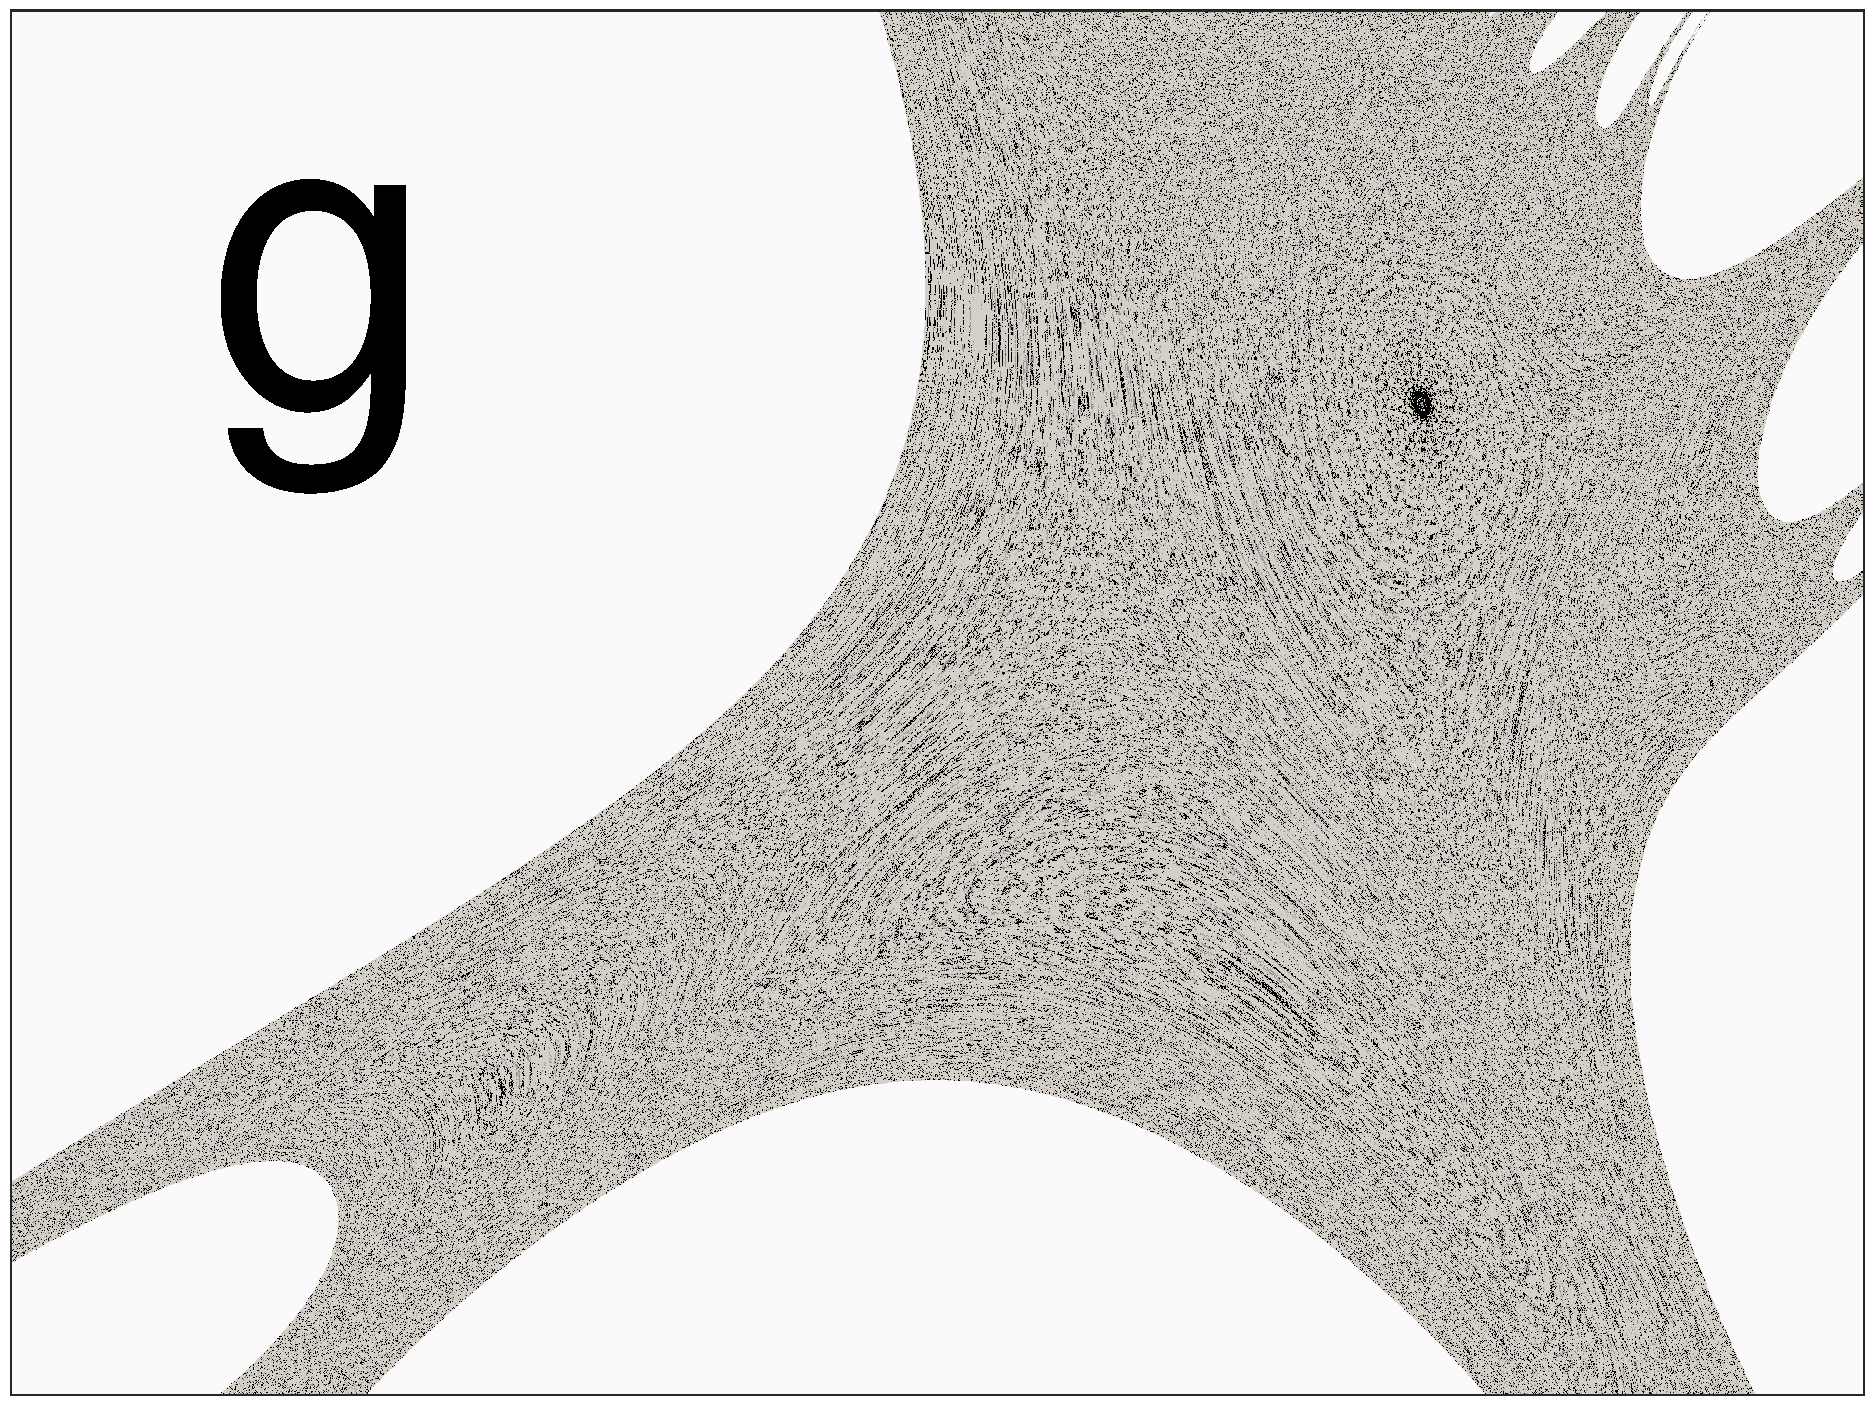
\includegraphics[width=0.3\textwidth]{m11_lu}
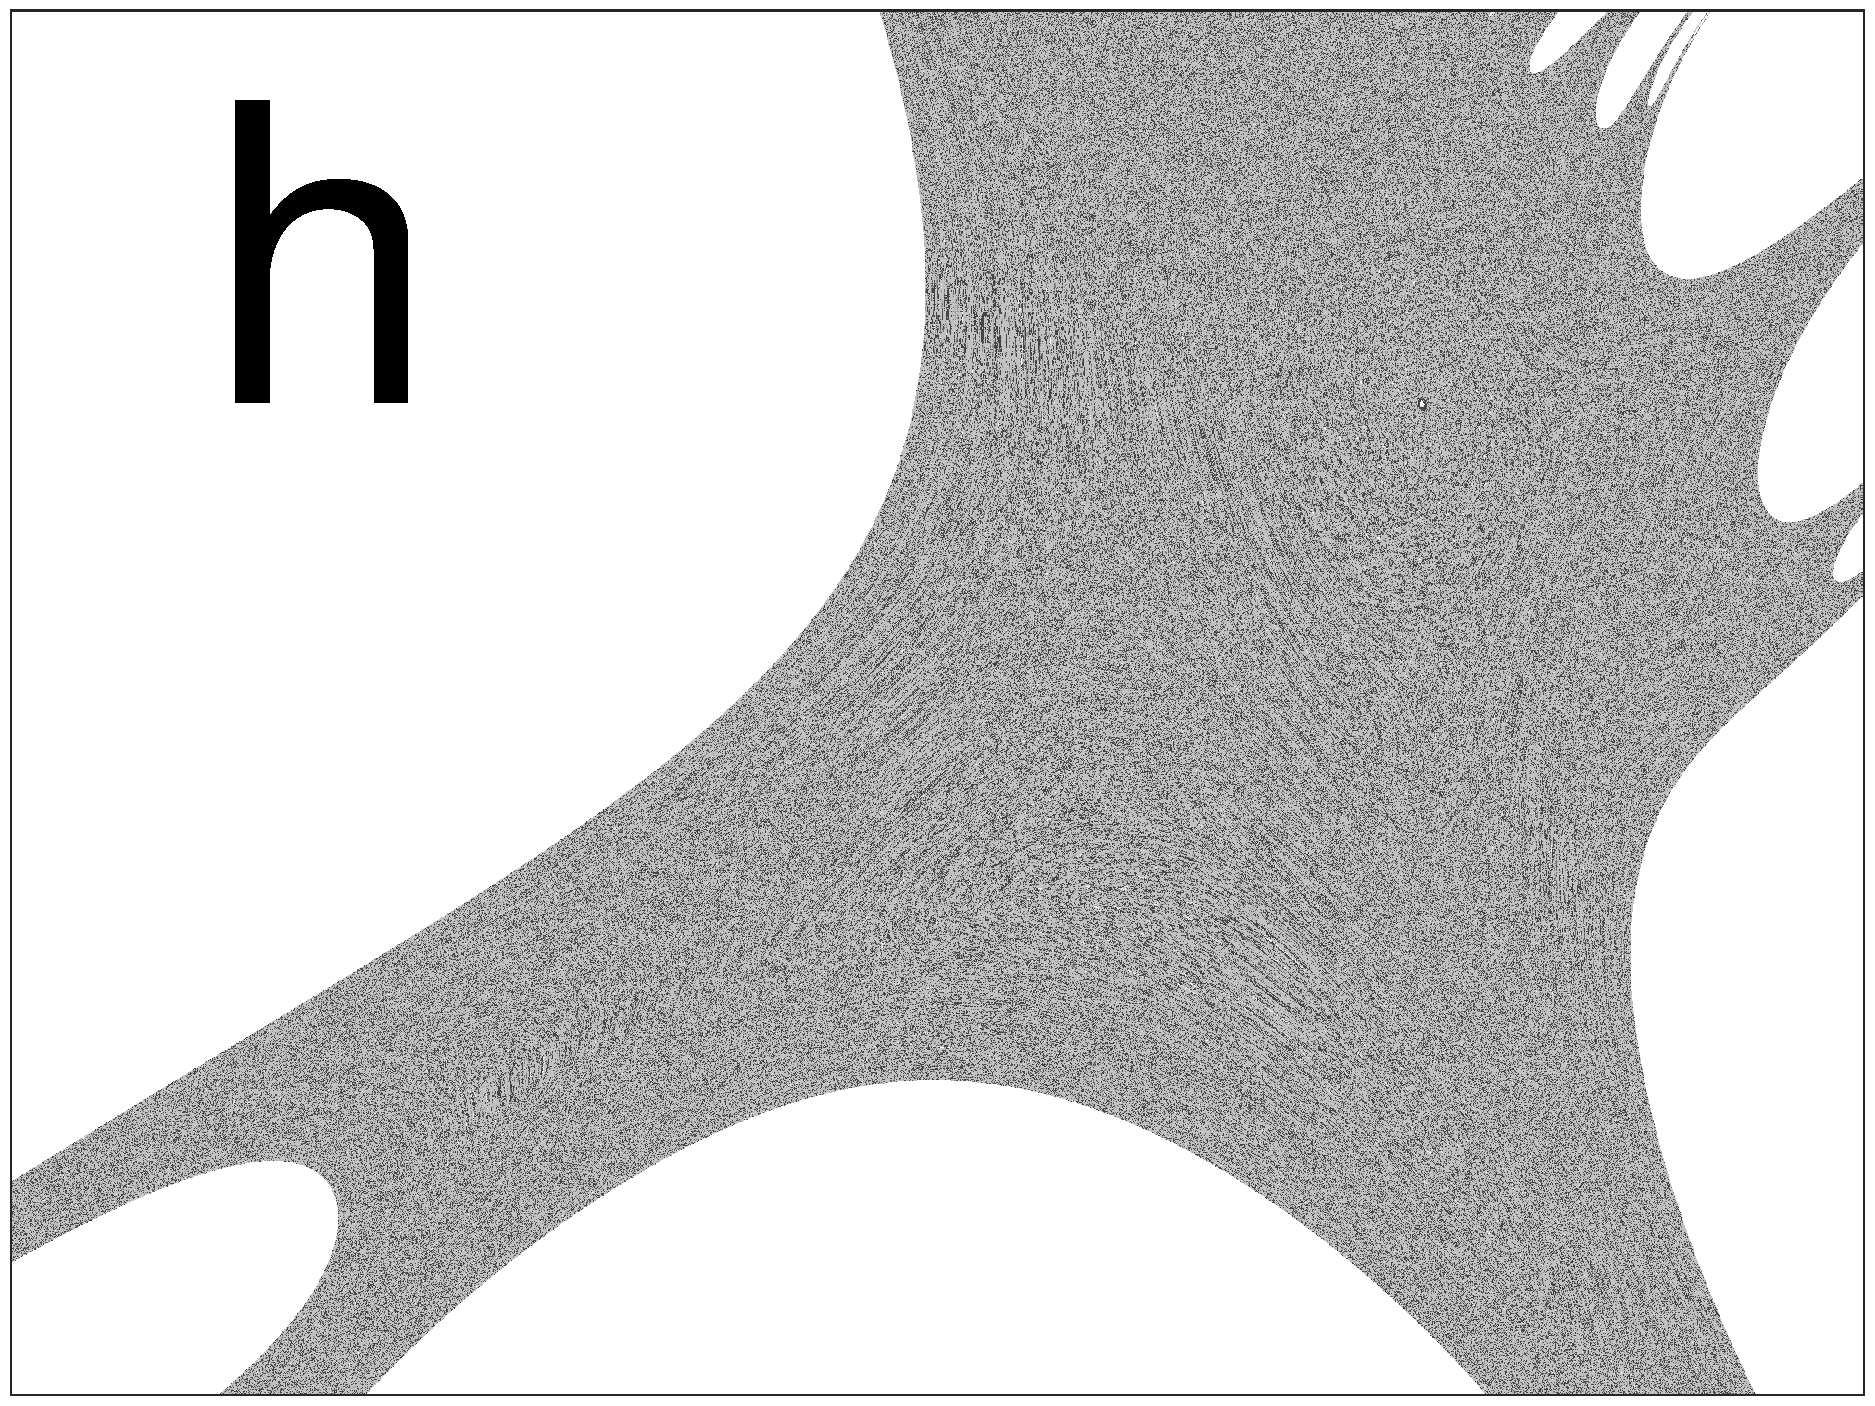
\includegraphics[width=0.3\textwidth]{m12_lu}
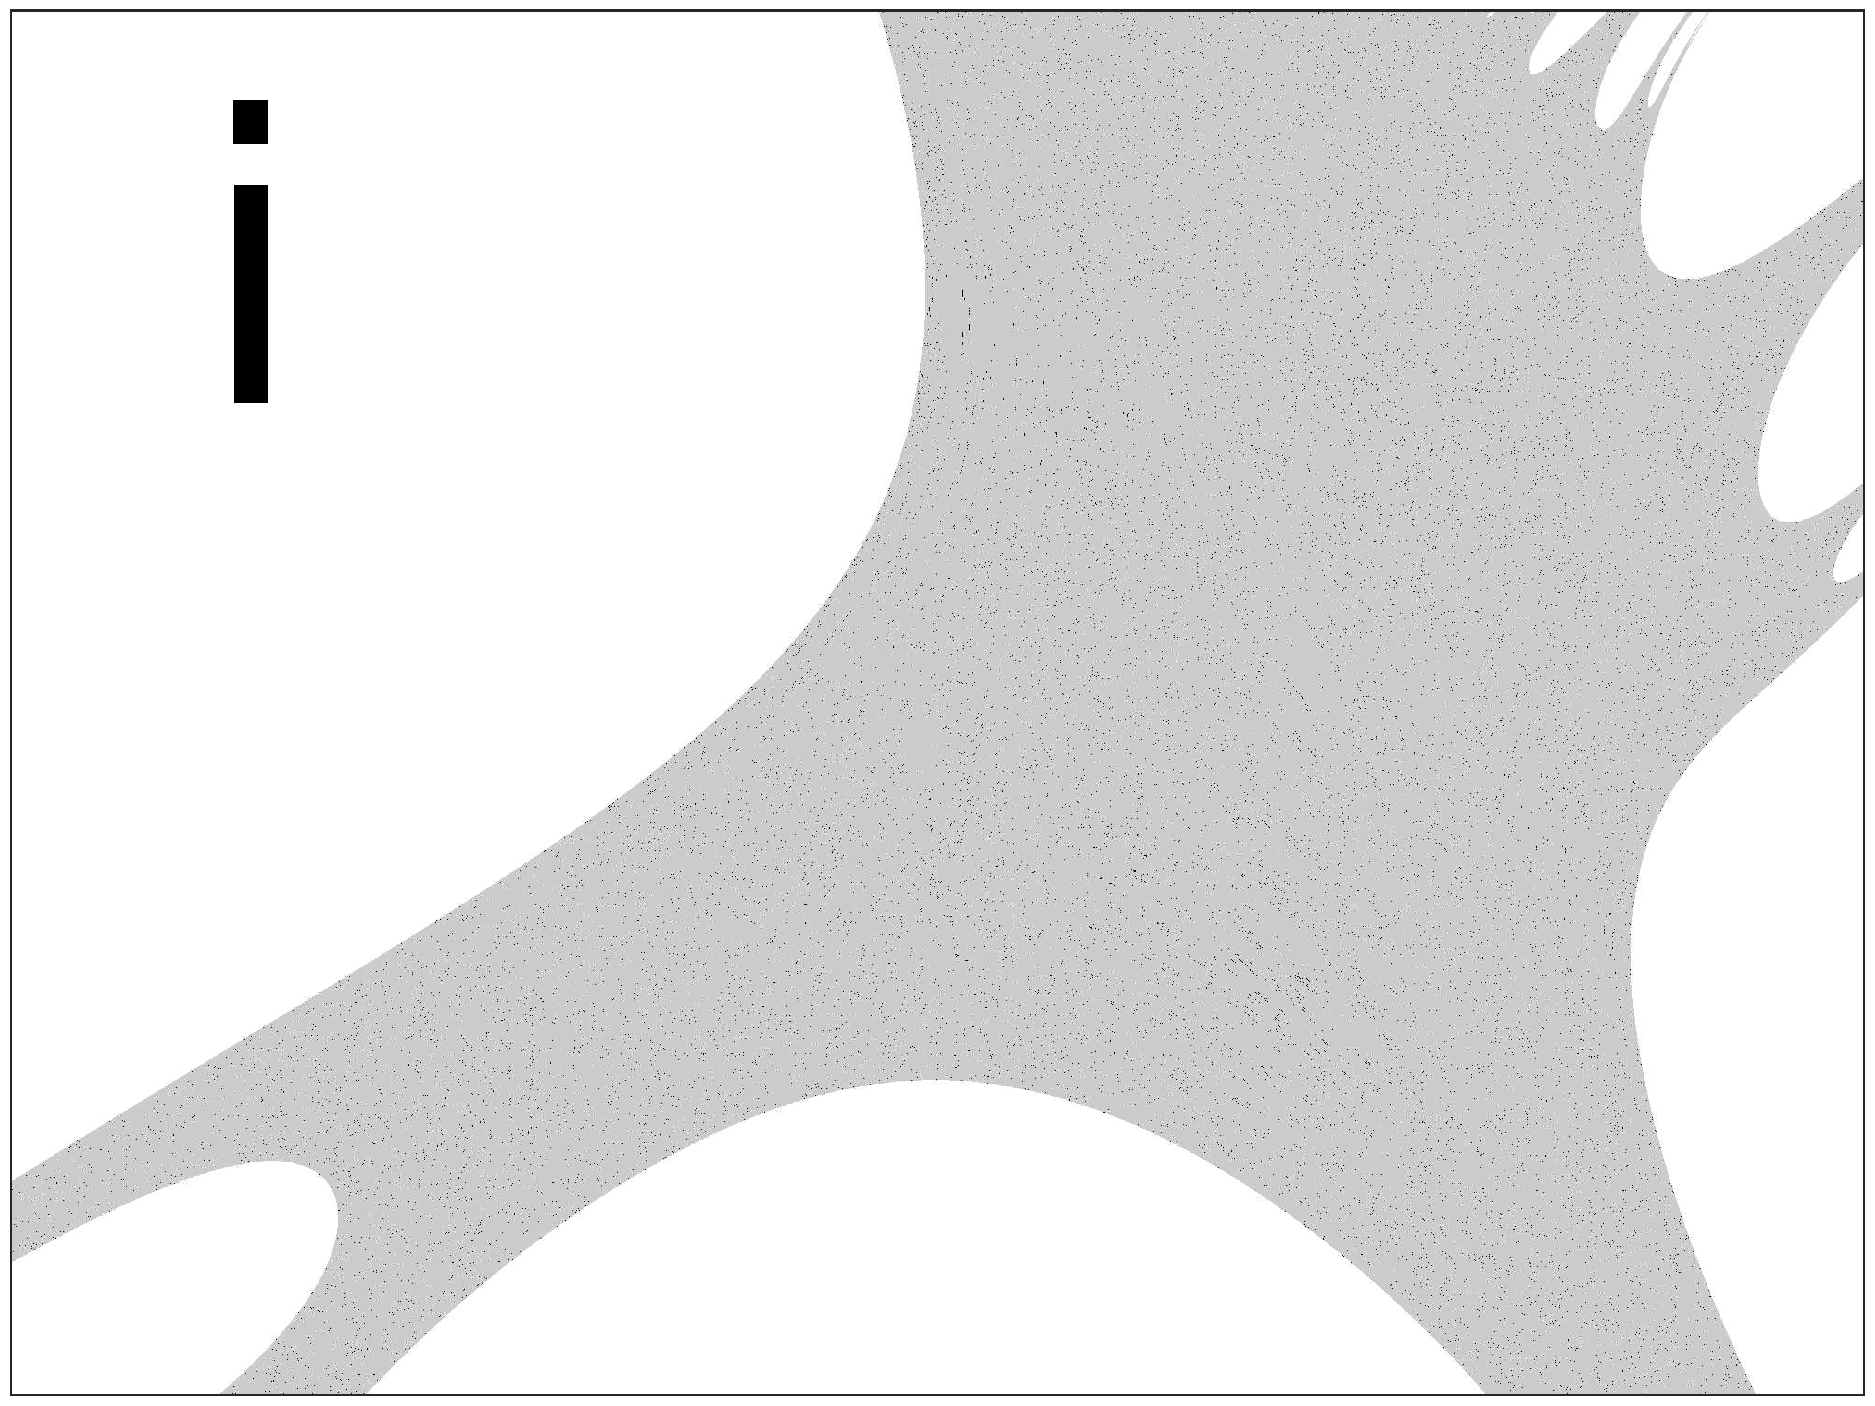
\includegraphics[width=0.3\textwidth]{m13_lu}\\
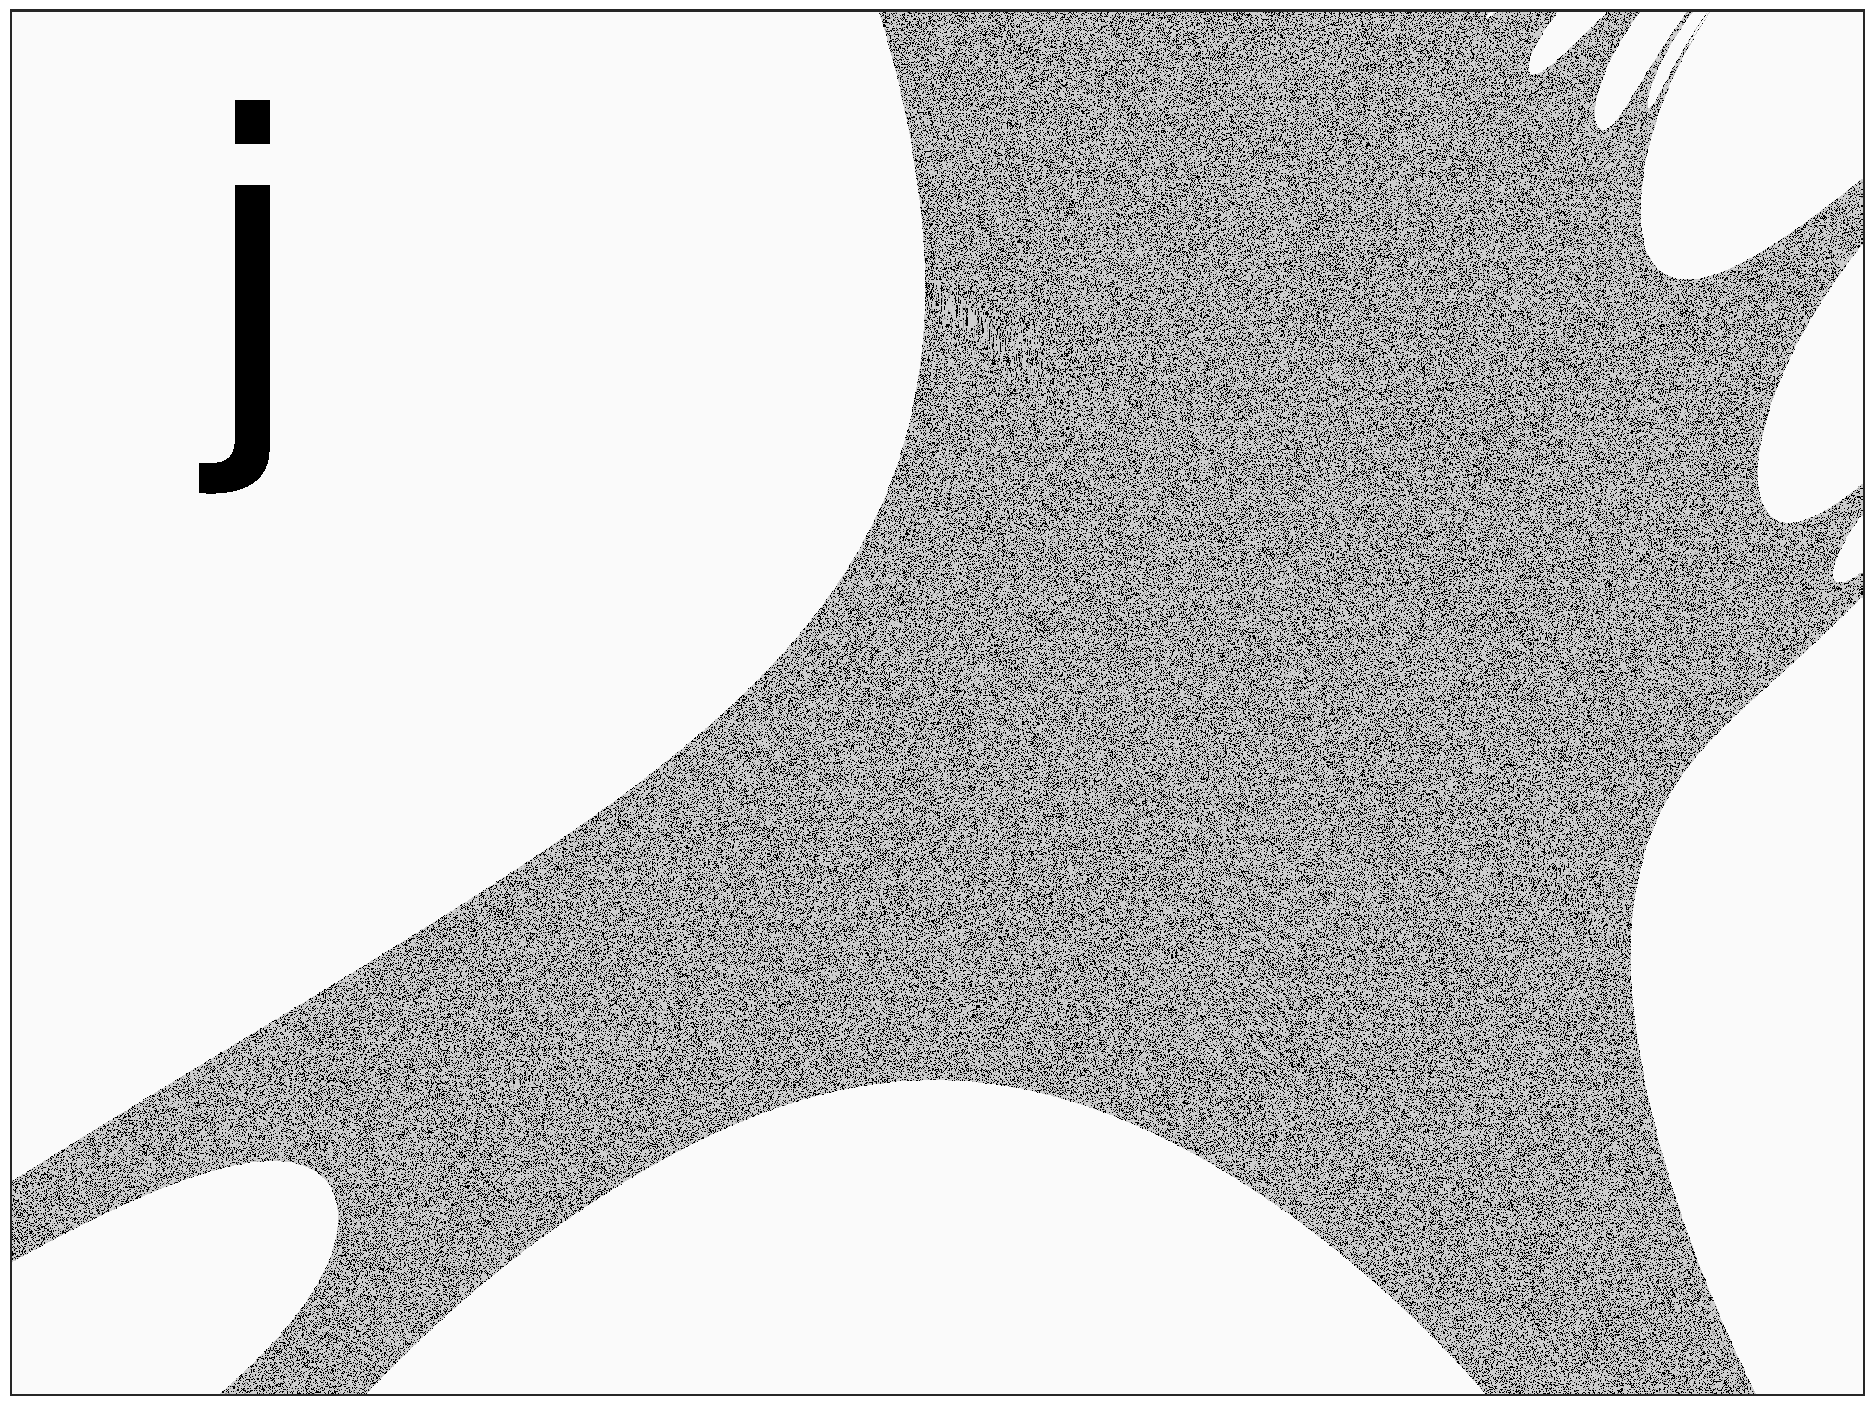
\includegraphics[width=0.3\textwidth]{m14_lu}
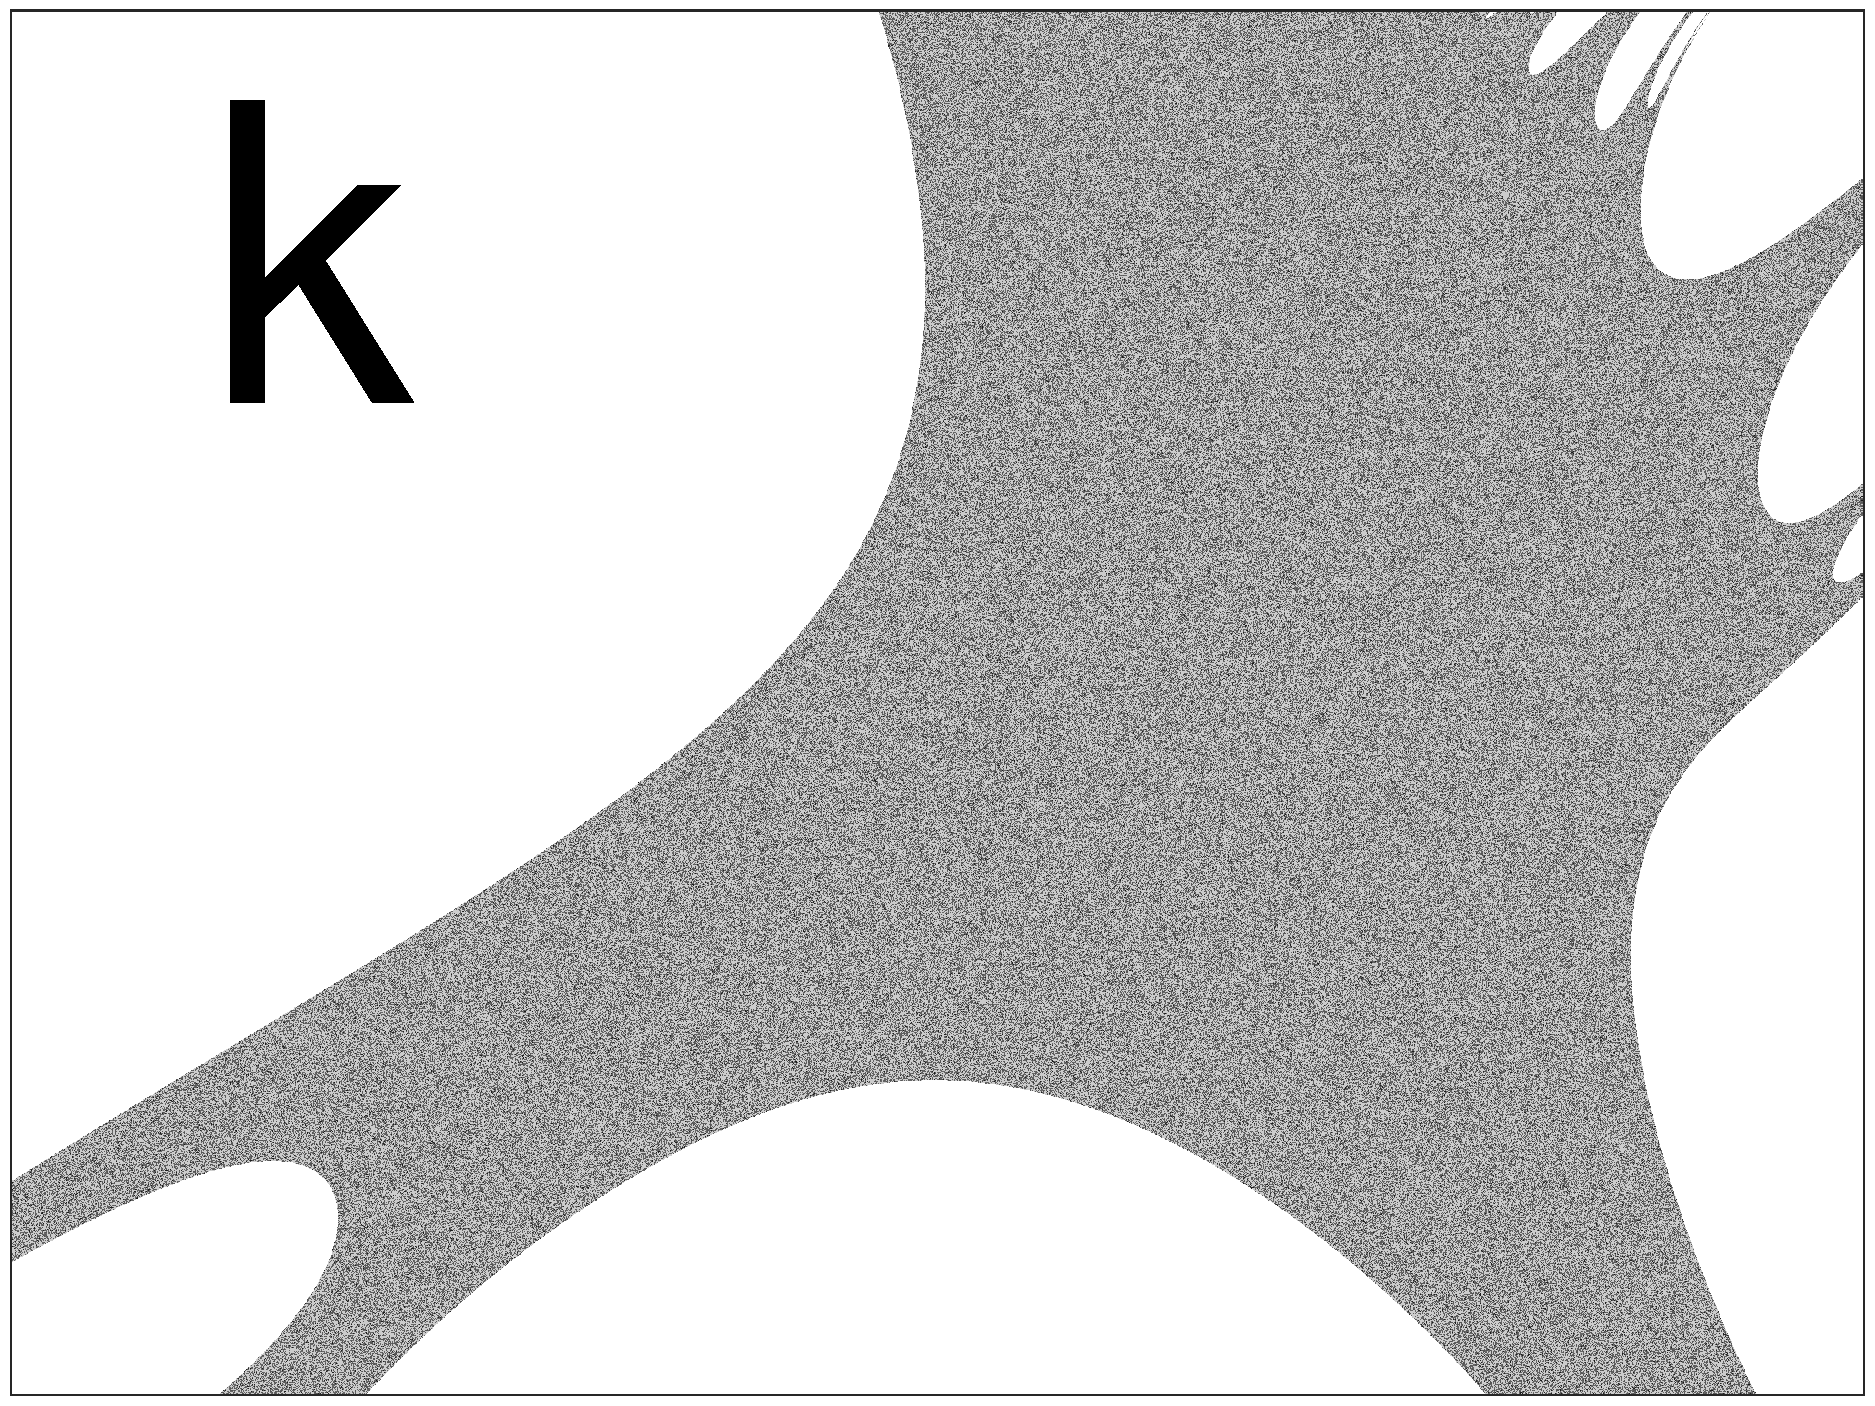
\includegraphics[width=0.3\textwidth]{m17_lu}
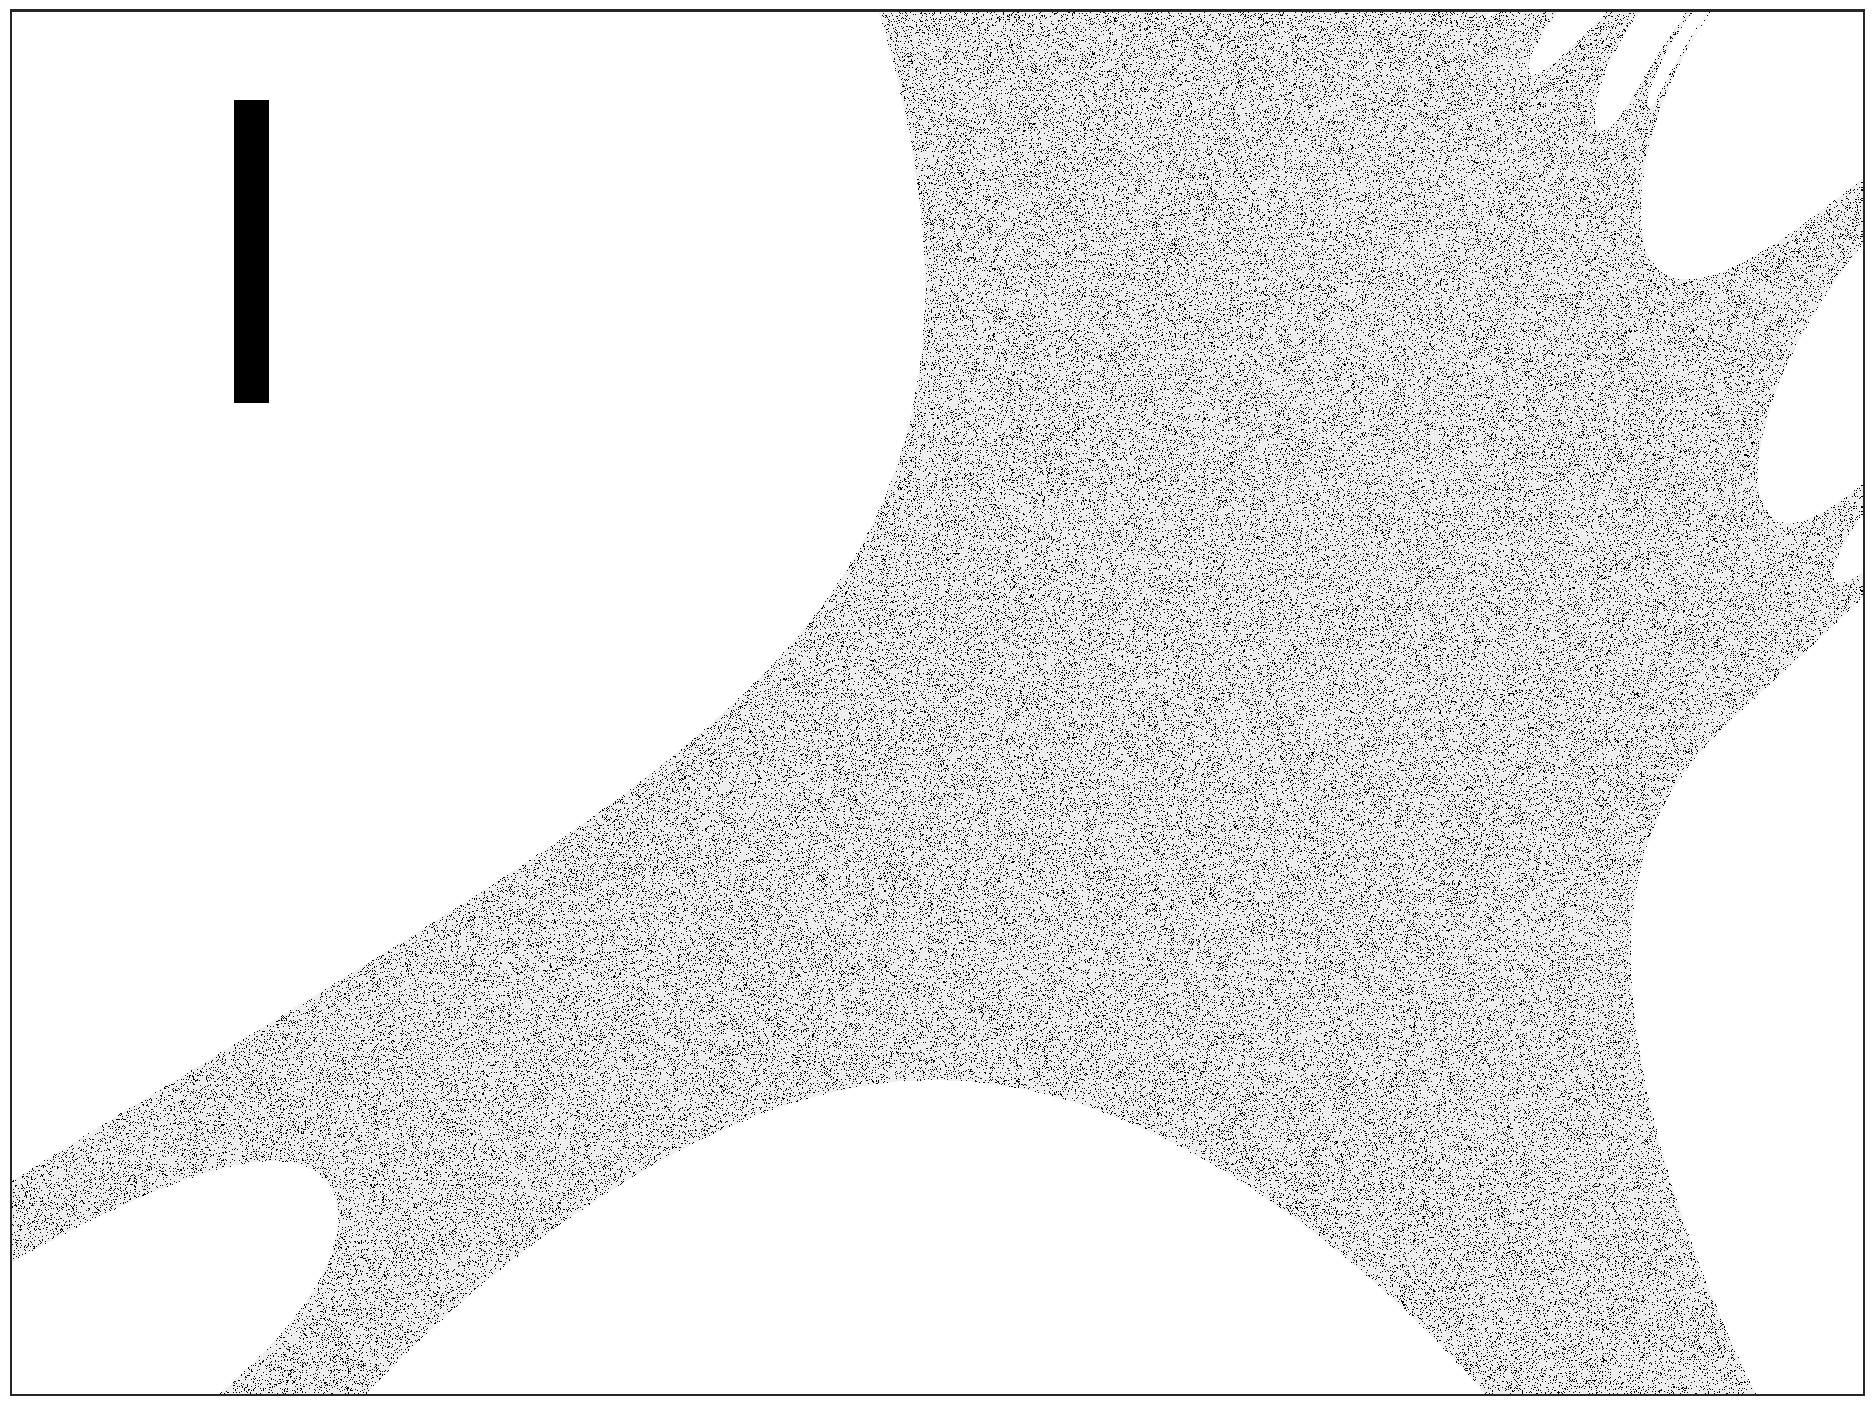
\includegraphics[width=0.3\textwidth]{m18_lu}\\
%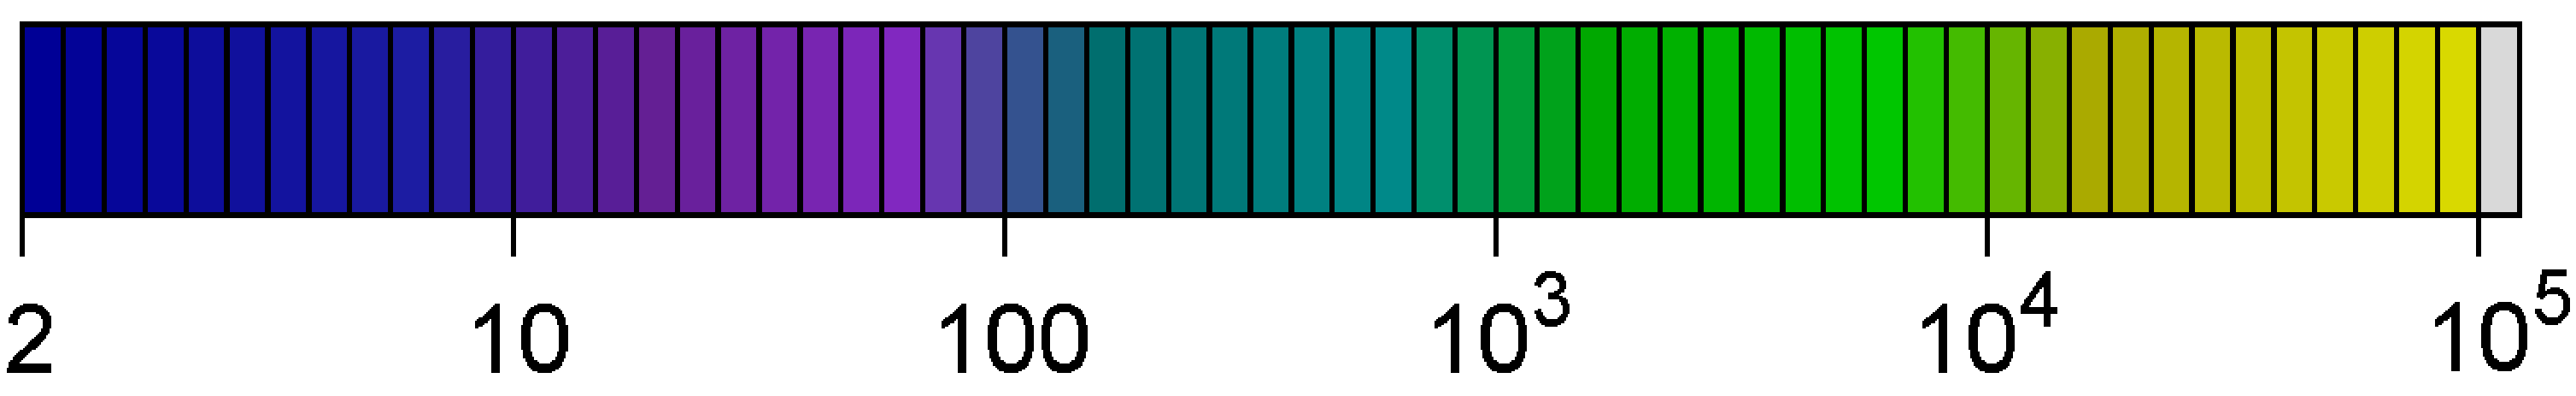
\includegraphics[width=1\textwidth]{ColorMapConEje}
\end{tabular}
\caption{Coexisting areas in attraction domains for: (a) $n_f=5$, (b) $n_f=6$, (c) $n_f=7$, (d) $n_f=8$, (e) $n_f=9$, (f) $n_f=10$, (g) $n_f=11$, (h) $n_f=12$, (i) $n_f=13$, (j) $n_f=14$, (k) $n_f=17$, (l) $n_f=18$.}
\label{fig:avvelo}
\end{figure}

With the purpose of being able to distinguish the different coexisting areas, a diverse range of gray tones have been used on each figure. It must be taken into account that each figure has its own gray range, this means that, for example, an almost white area when $n_f = 5$ (Fig. \ref{fig:avvelo}.a) corresponds to a period of $6$, while a darker area in a figure with higher $n_f$ may correspond to a period higher than a thousand (Fig. \ref{fig:avvelo}.e). These figures allow reflecting the  complex domains of attraction that appear when digitalizing.

It can be seen in Fig. \ref{fig:avvelo} that the smaller the value of $n_f$ the bigger the area of ICs that tends to diverge and to converge to fixed points. As $n_f$ increases, the area of divergent and fixed points decreases.
These figures along with Table \ref{tabla} allows an easy interpretation of the system's behavior. In Table \ref{tabla} the period's lengths that appear in the attractor domain for every $n_f$ are sorted by the more to the less numerous ICs that converges to that cycle. In parentheses it can be seen the percent of occurrence.
Indeed, figures with lower values of $n_f$ present irregular, or rough surfaces, pointing out that different lengths cycles coexist there. For example, for $n_f=5$ there is a prevalence of  short periods cycles. In that case, there exist just two limit cycles, the lighter grey zone corresponds to the attraction domain of the limit cycles of length six, that is the less numerous cycle, according to Table \ref{tabla}, and, the darker zone corresponds to the attraction domain of length two cycle.

Although for $n_f \geqslant 13$ (Figures \ref{fig:avvelo}.i to \ref{fig:avvelo}.l) the attractor appears to be smooth and uniform, however, if a \emph{zoom in} is done to the figures (Fig. \ref{fig:m_zoom}) it can be seen that there are still  cycles with different periods that coexist in the attractor for $n_f=14$,$17$ and $18$.


%==========================zooms in============================
\begin{figure}
\begin{tabular}{cc}
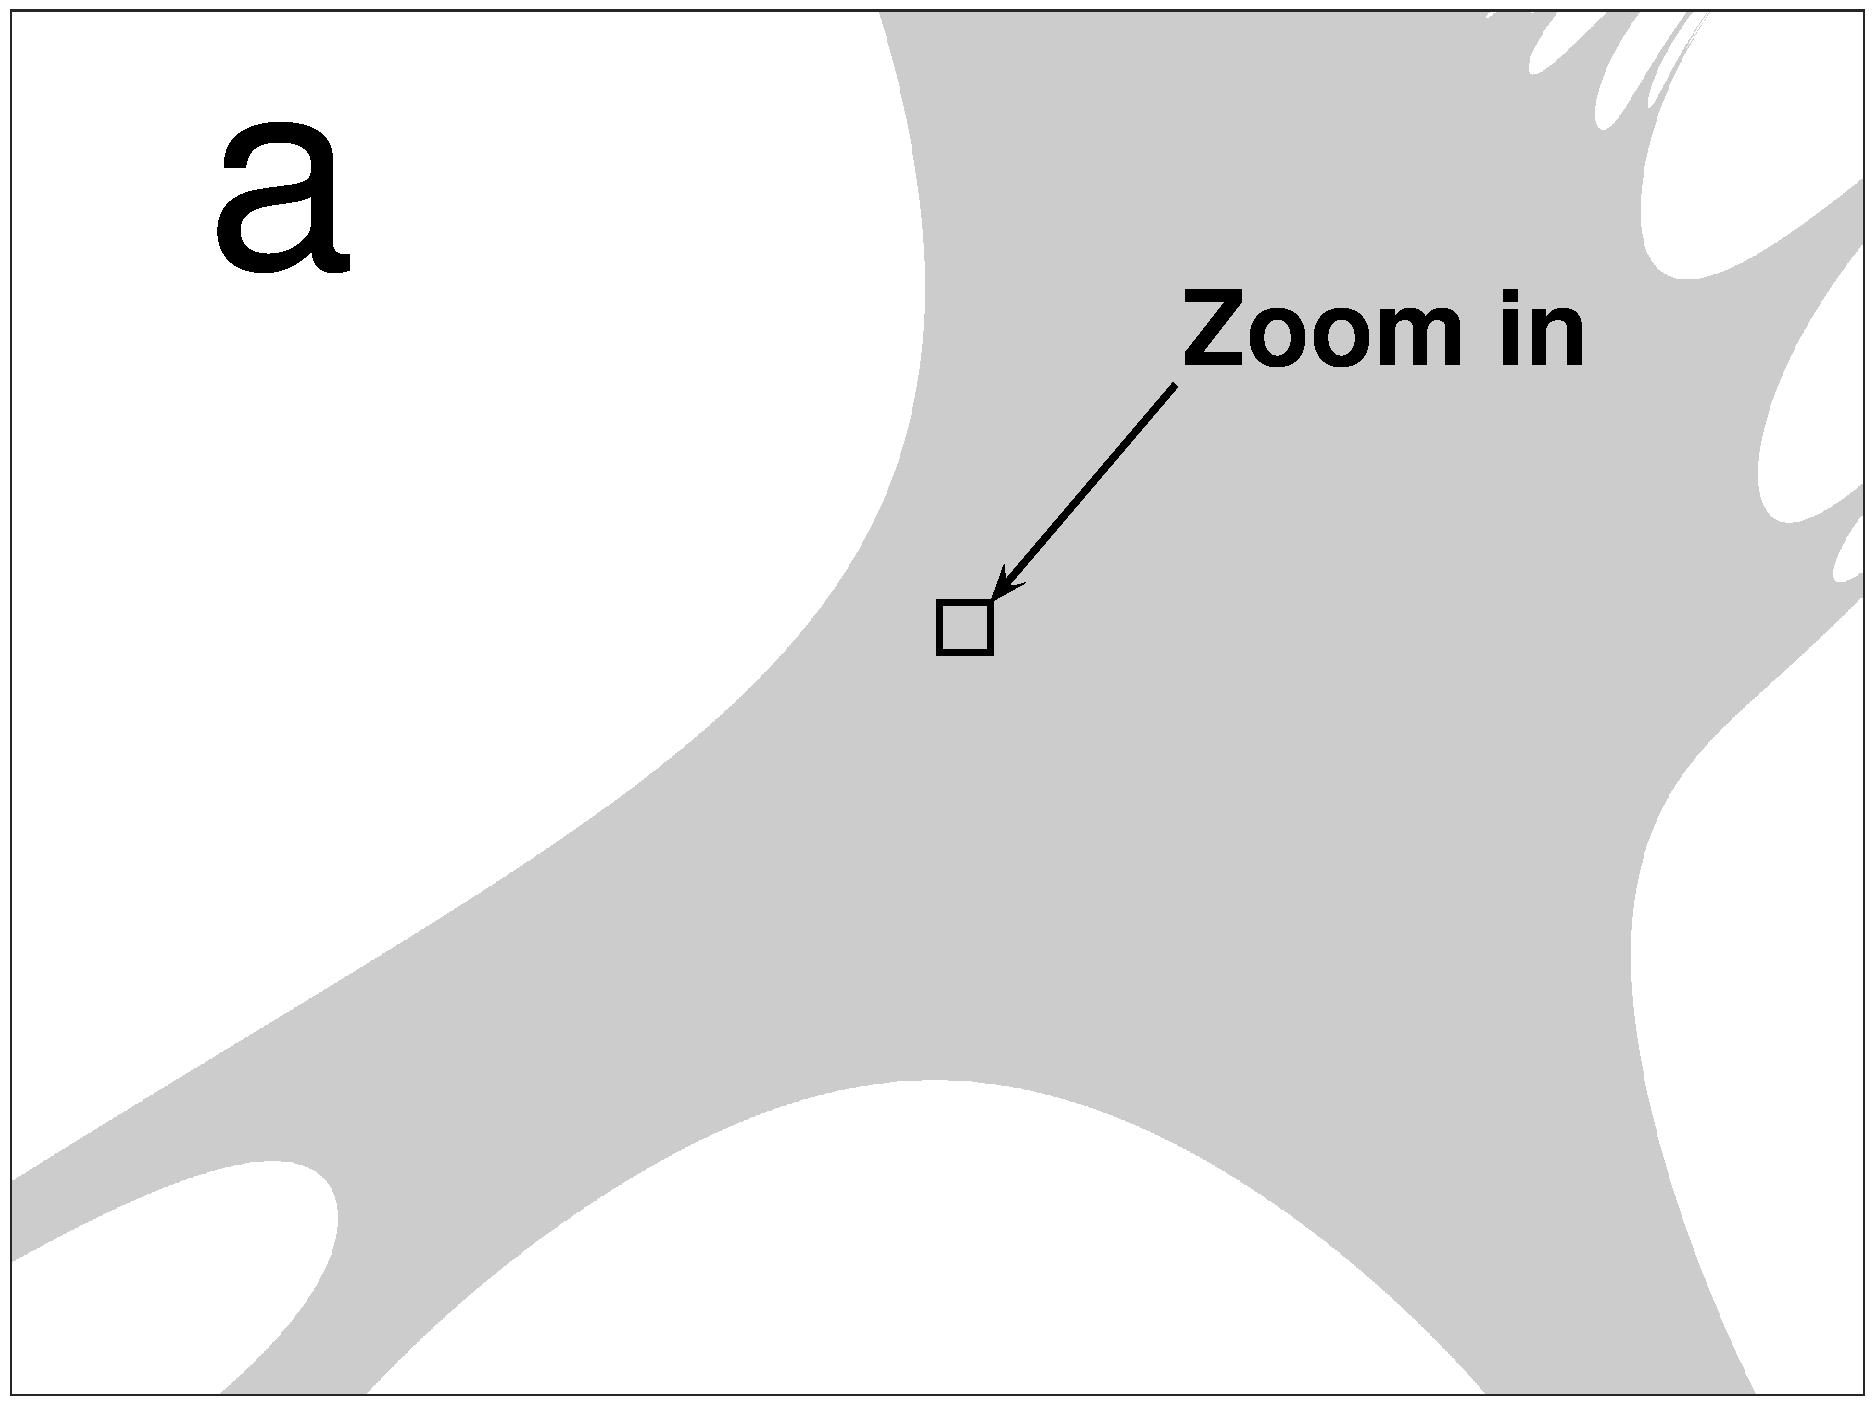
\includegraphics[width=0.48\textwidth]{m_zoom}
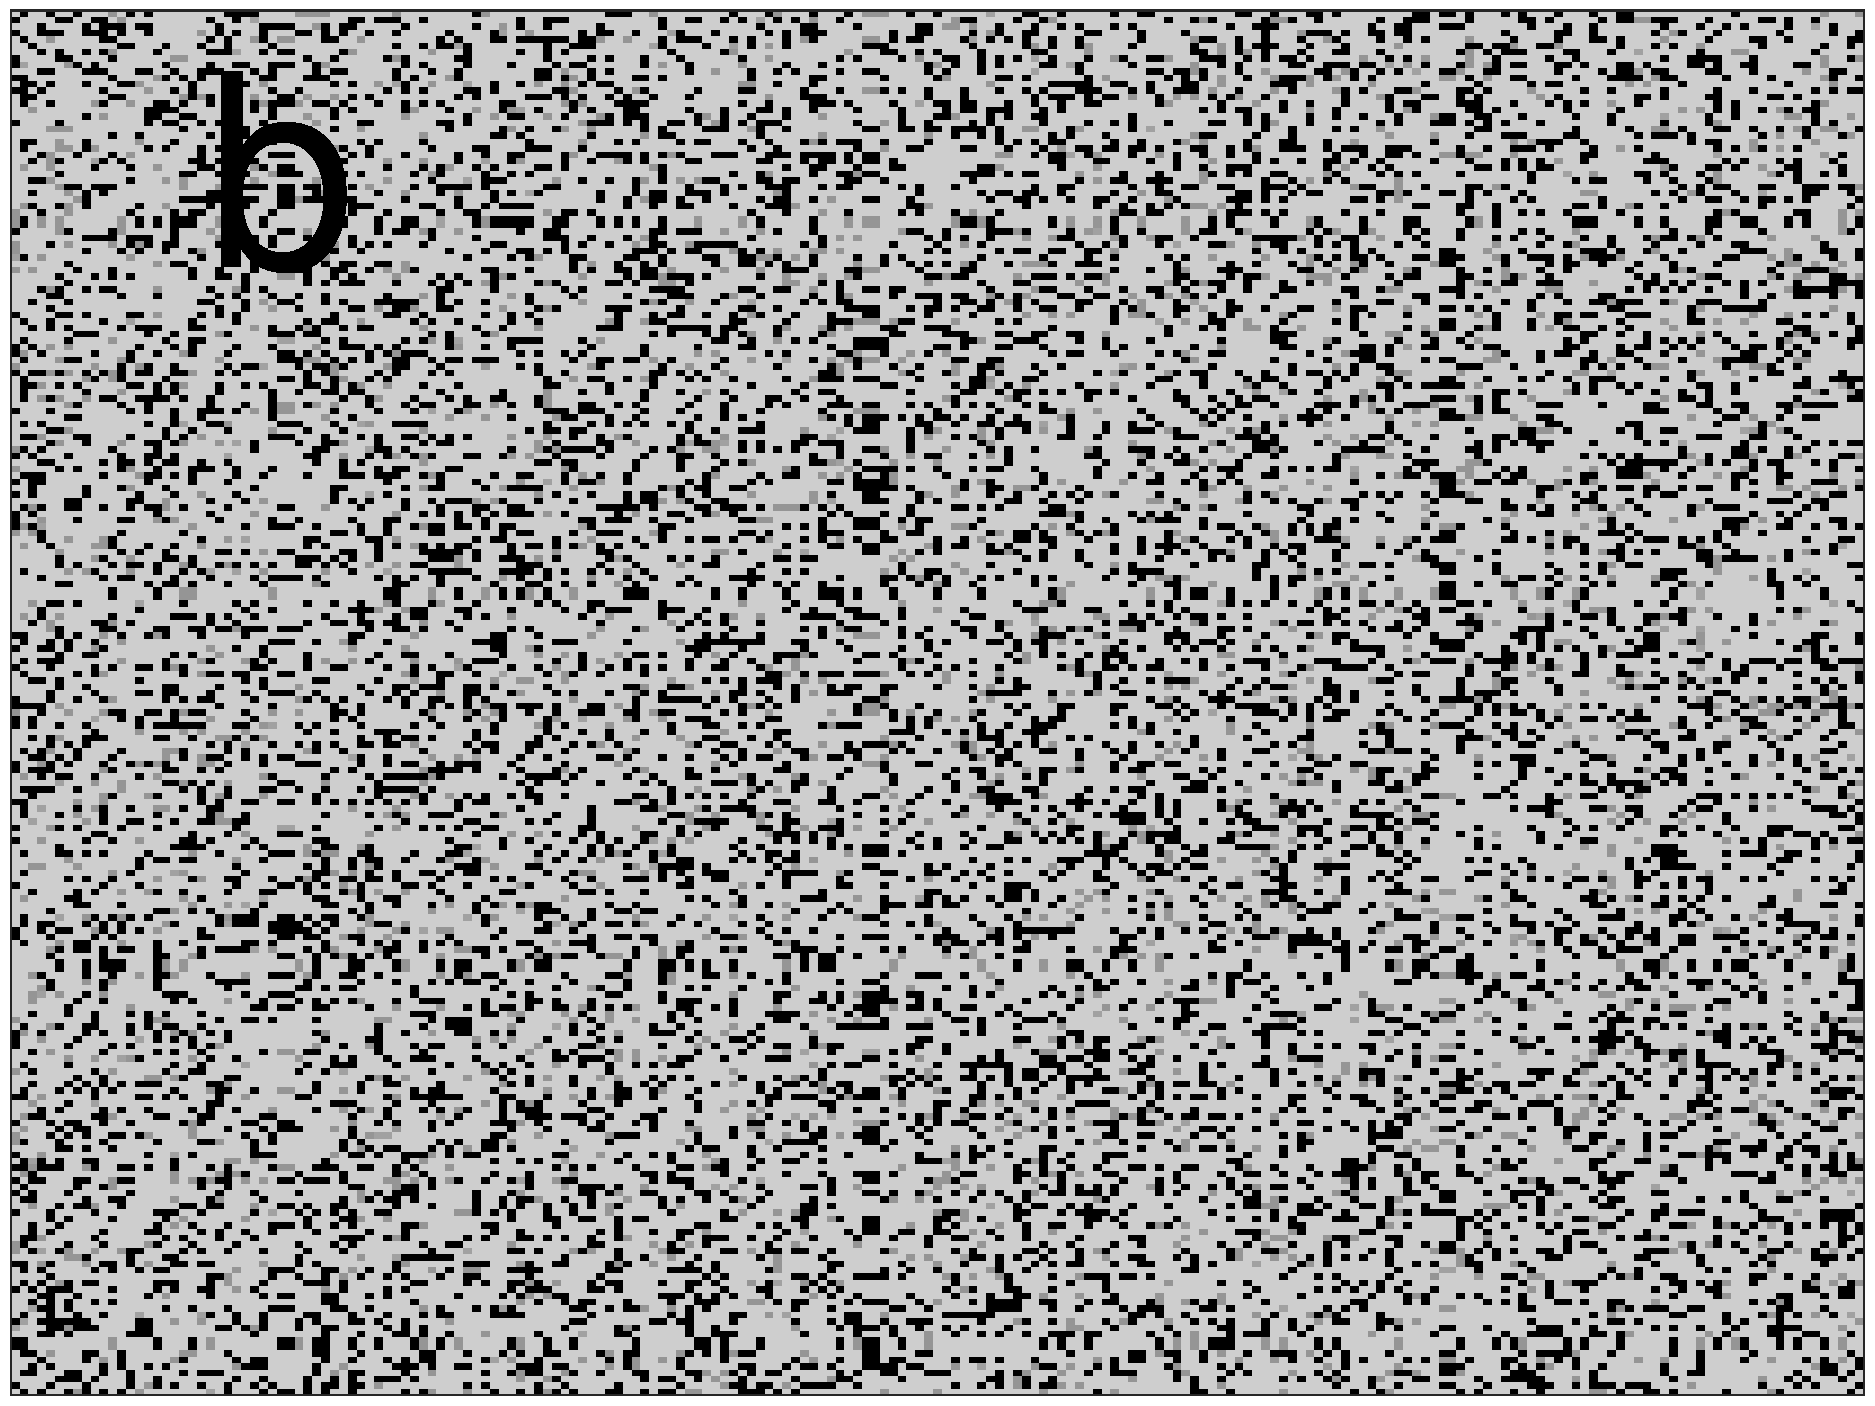
\includegraphics[width=0.48\textwidth]{m14_lu_zoom}\\
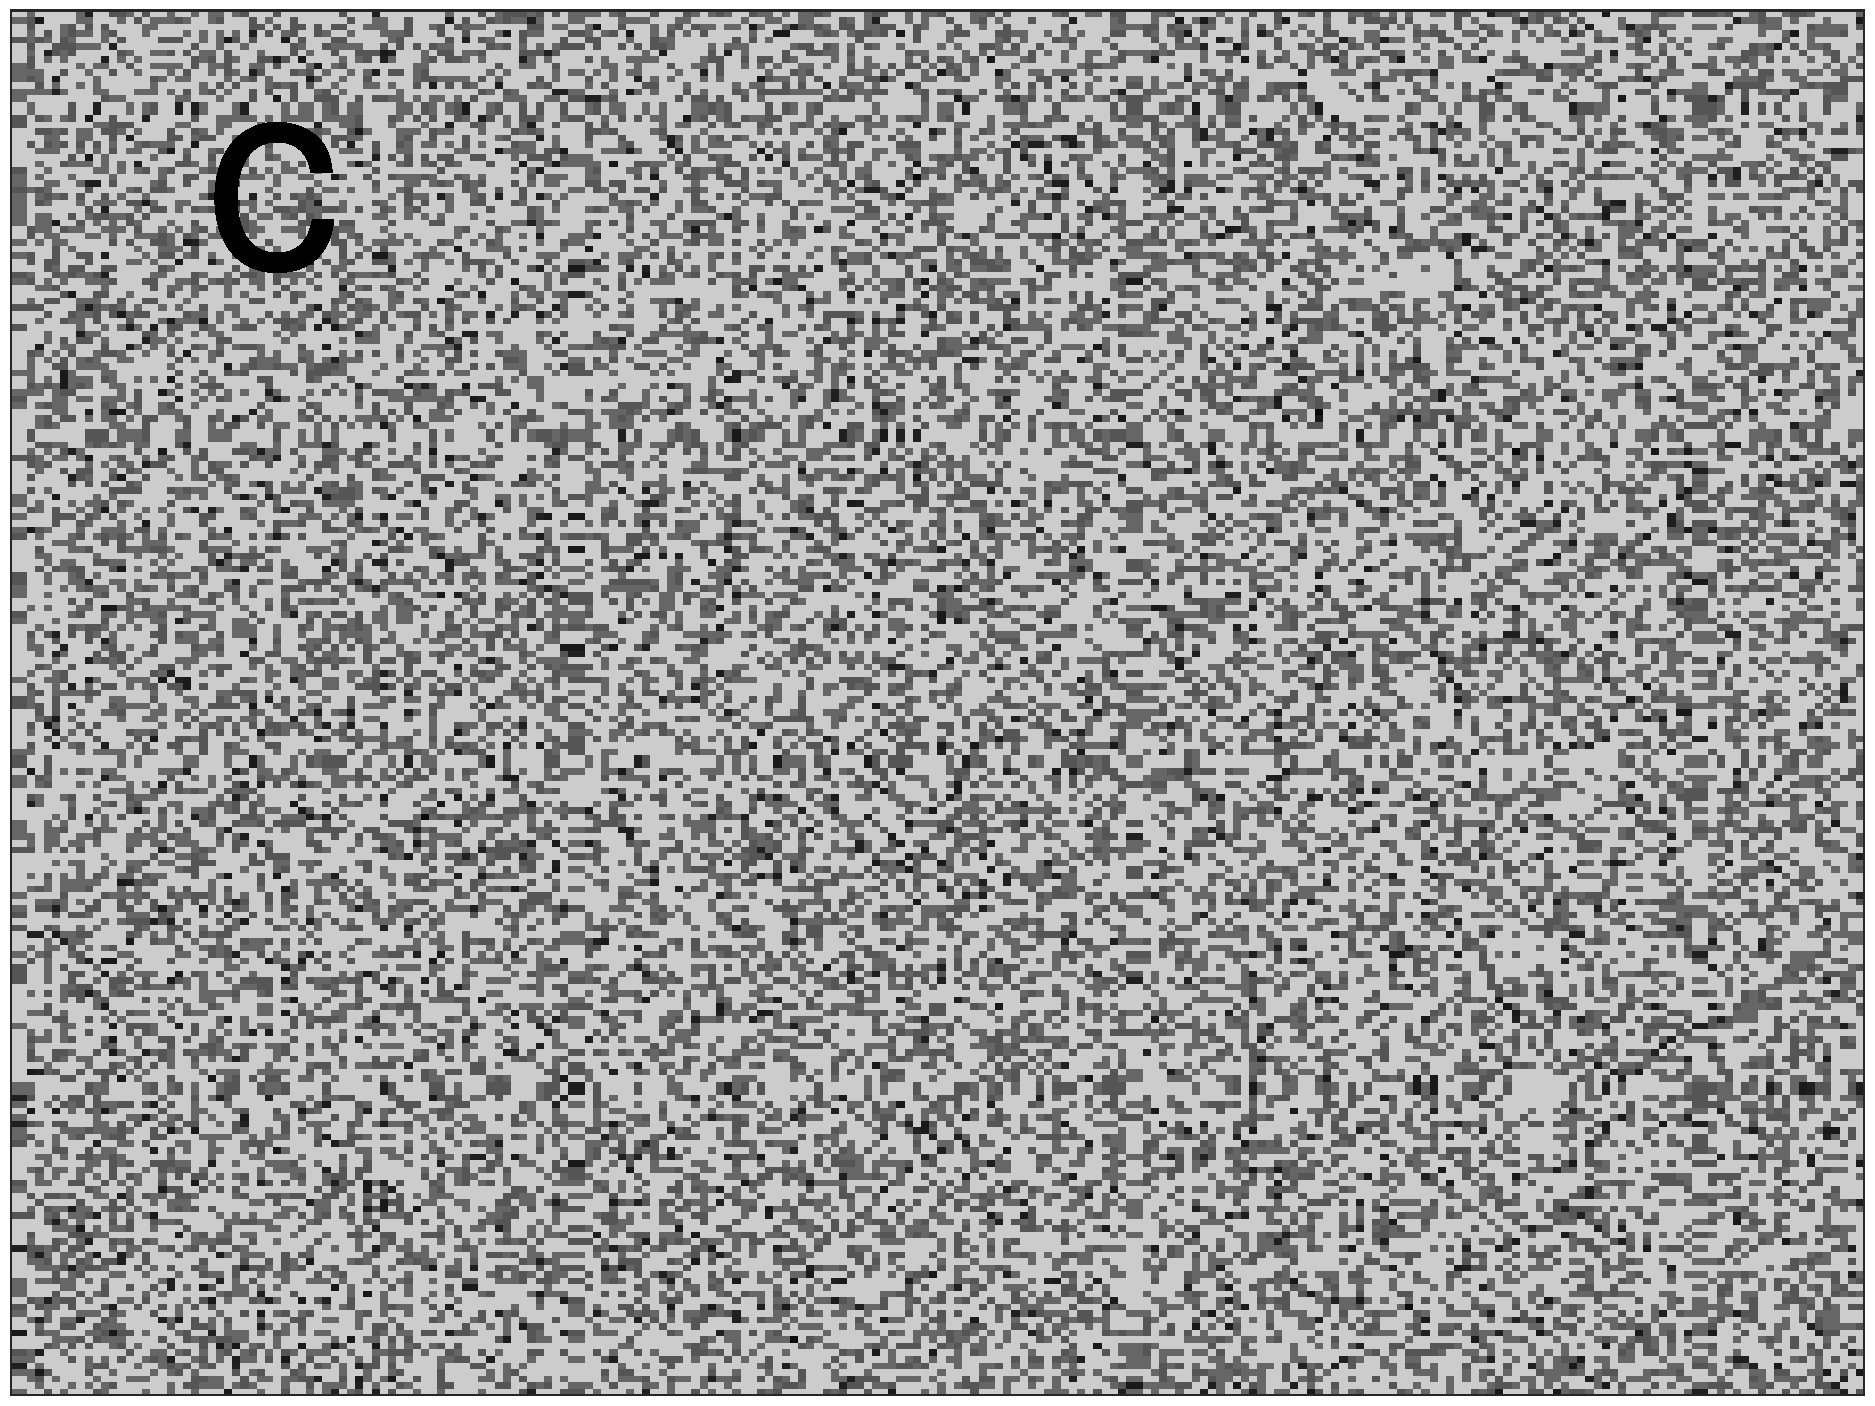
\includegraphics[width=0.48\textwidth]{m17_lu_zoom}
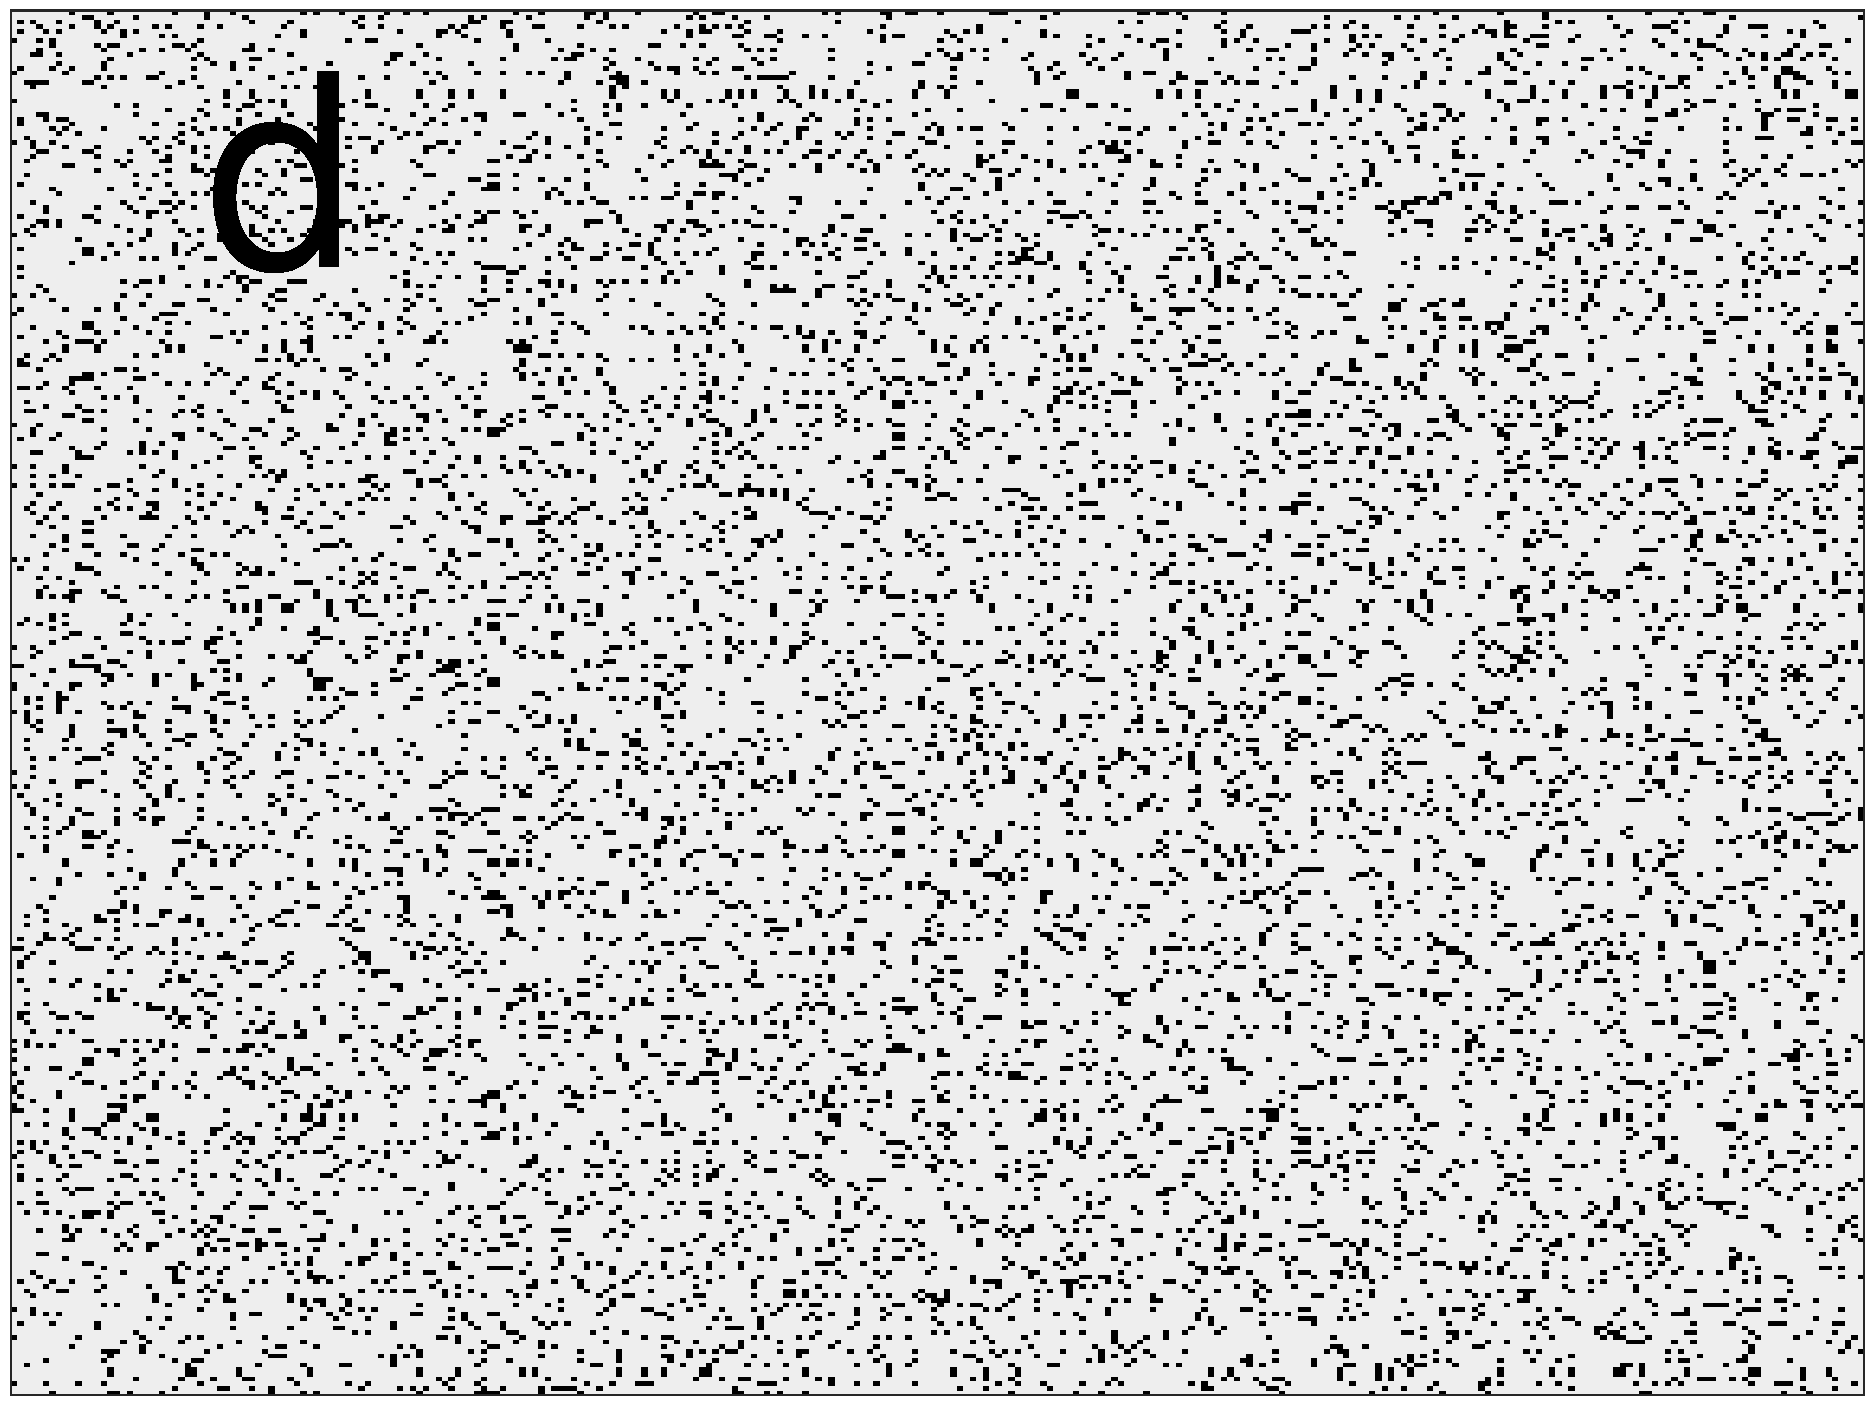
\includegraphics[width=0.48\textwidth]{m18_lu_zoom}
\end{tabular}
\caption{Enlarged views of sections of the attraction domains for higher values of $n_f$:
(a) Rectangular section of the attraction domain to be zoomed in; (b)  $n_f=14$ zoom; (c) $n_f=17$ zoom;  (d) $n_f=18$ zoom.}
\label{fig:m_zoom}
\end{figure}
%============================================================================================

Nevertheless, when we want to make a general comparison of what happens to the periods when the precisions are varied a color scale is required, see Fig. \ref{fig:m}.
% ==DOMINIOS DE ATRACCION DE ATRACTOR 2PARA DISTINTO NUMERO DE BITS  
% SALTEAMOS 15 Y 16 PORQUE DAN MUY PARECIDOS A 14 Y 17
\begin{figure}
\centering
\begin{tabular}{cc}
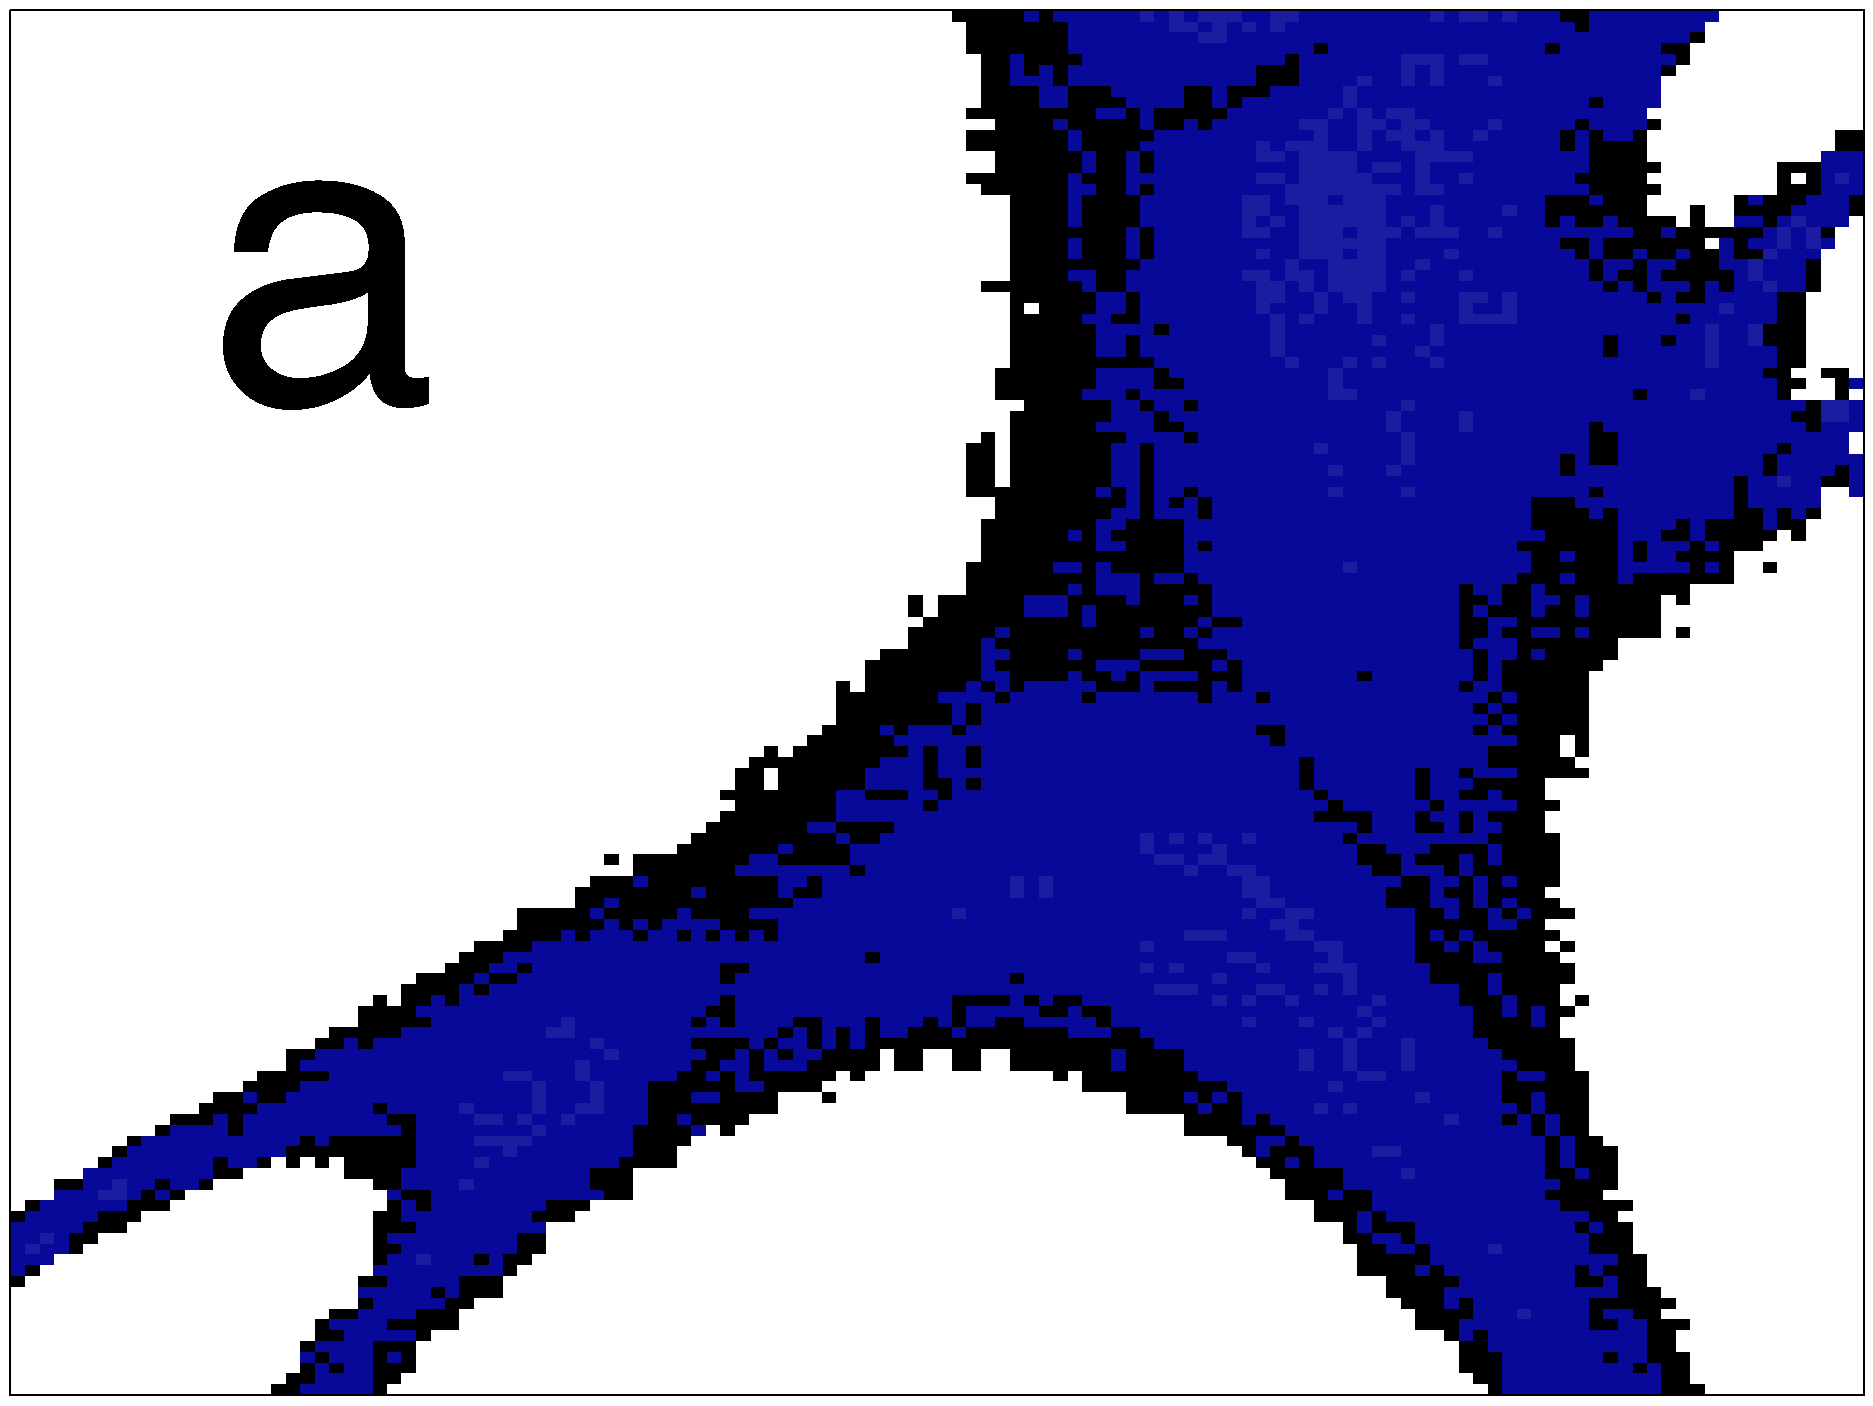
\includegraphics[width=0.3\textwidth]{m5}
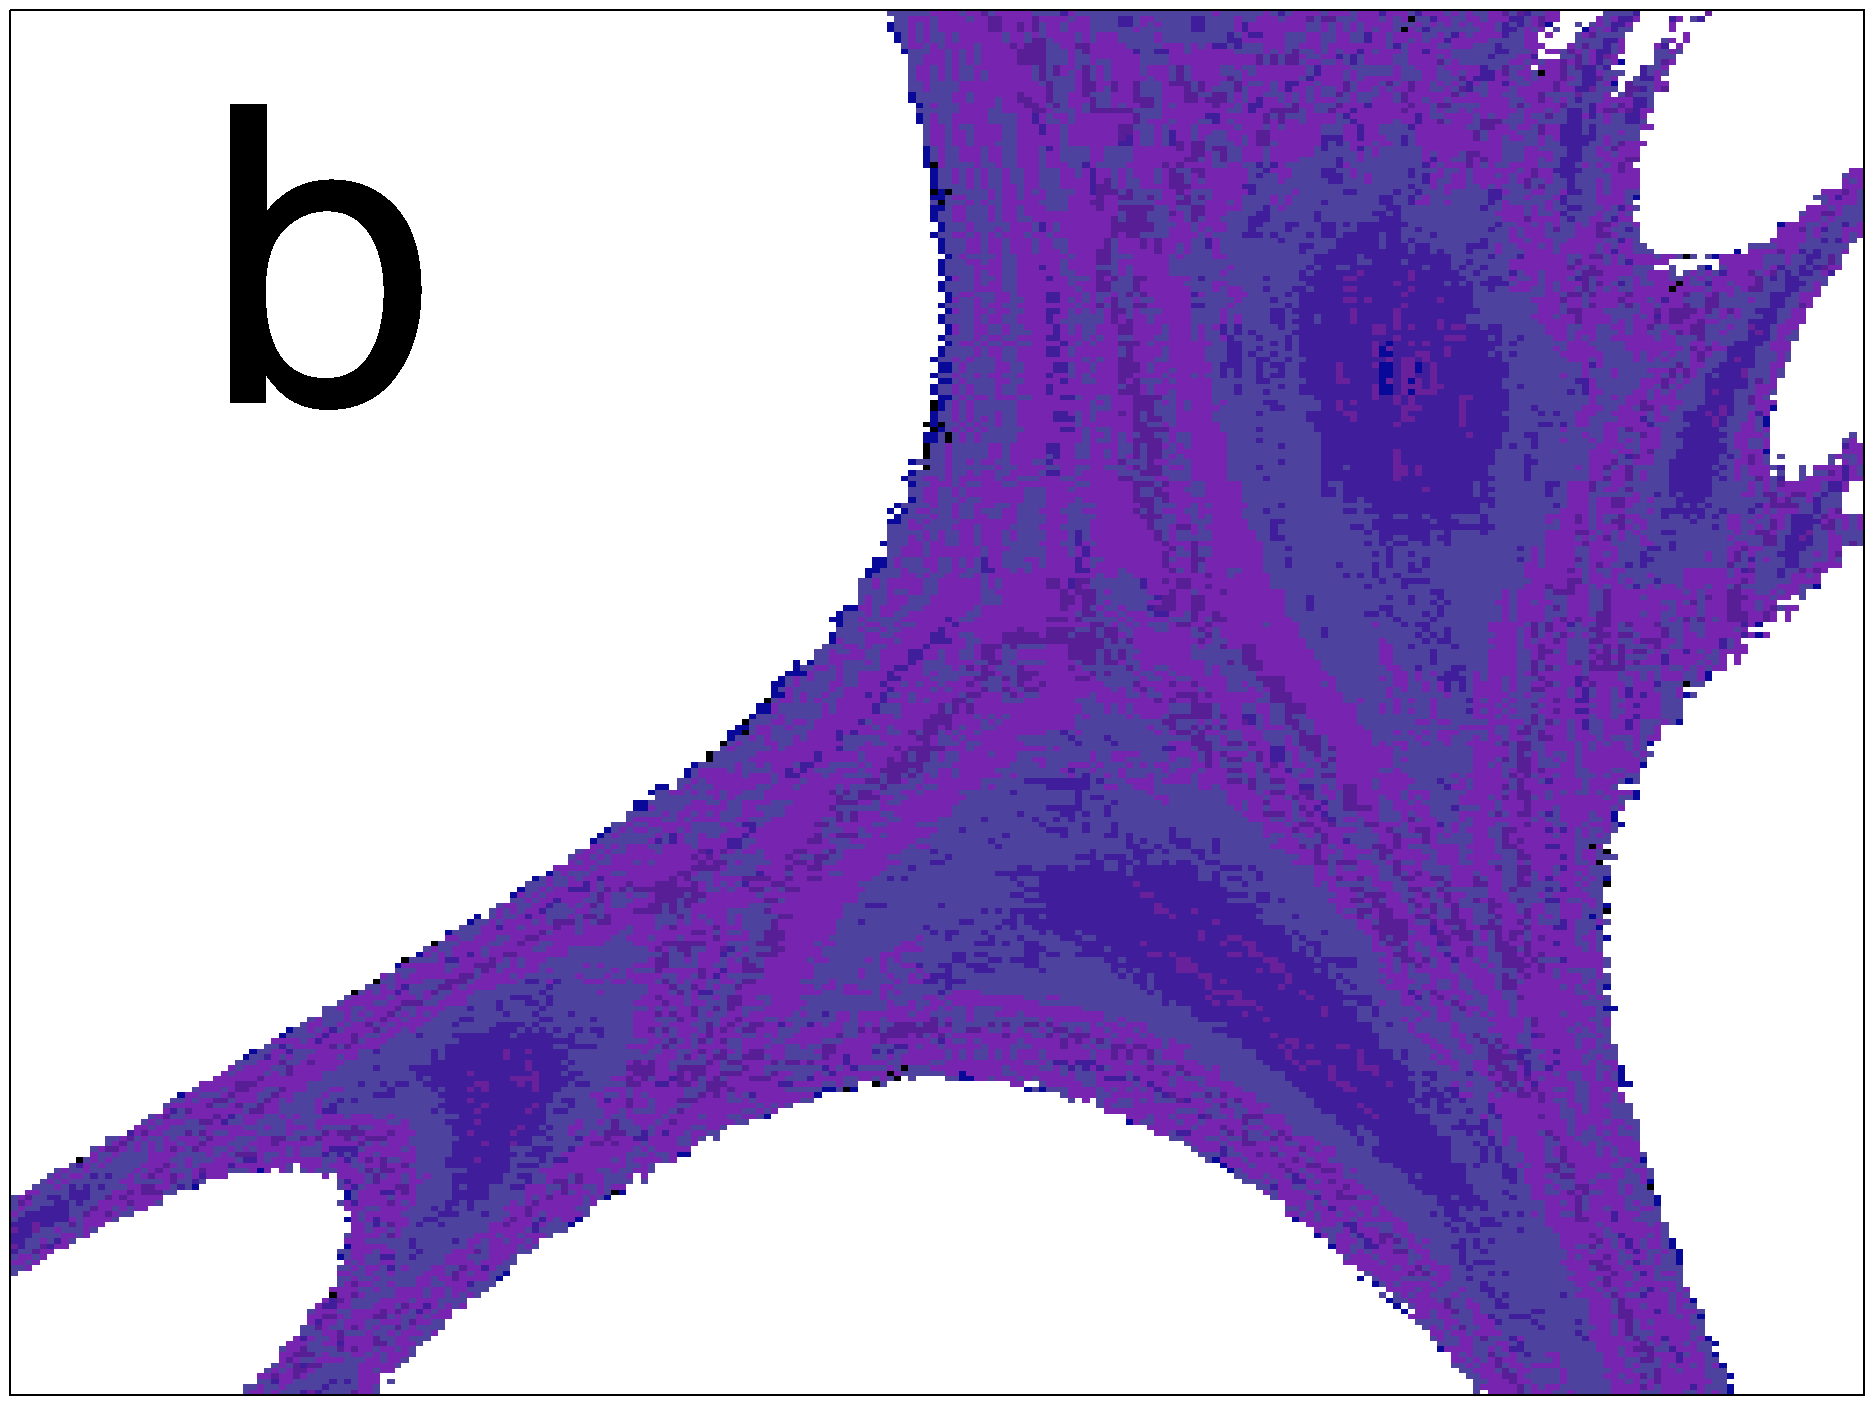
\includegraphics[width=0.3\textwidth]{m6}
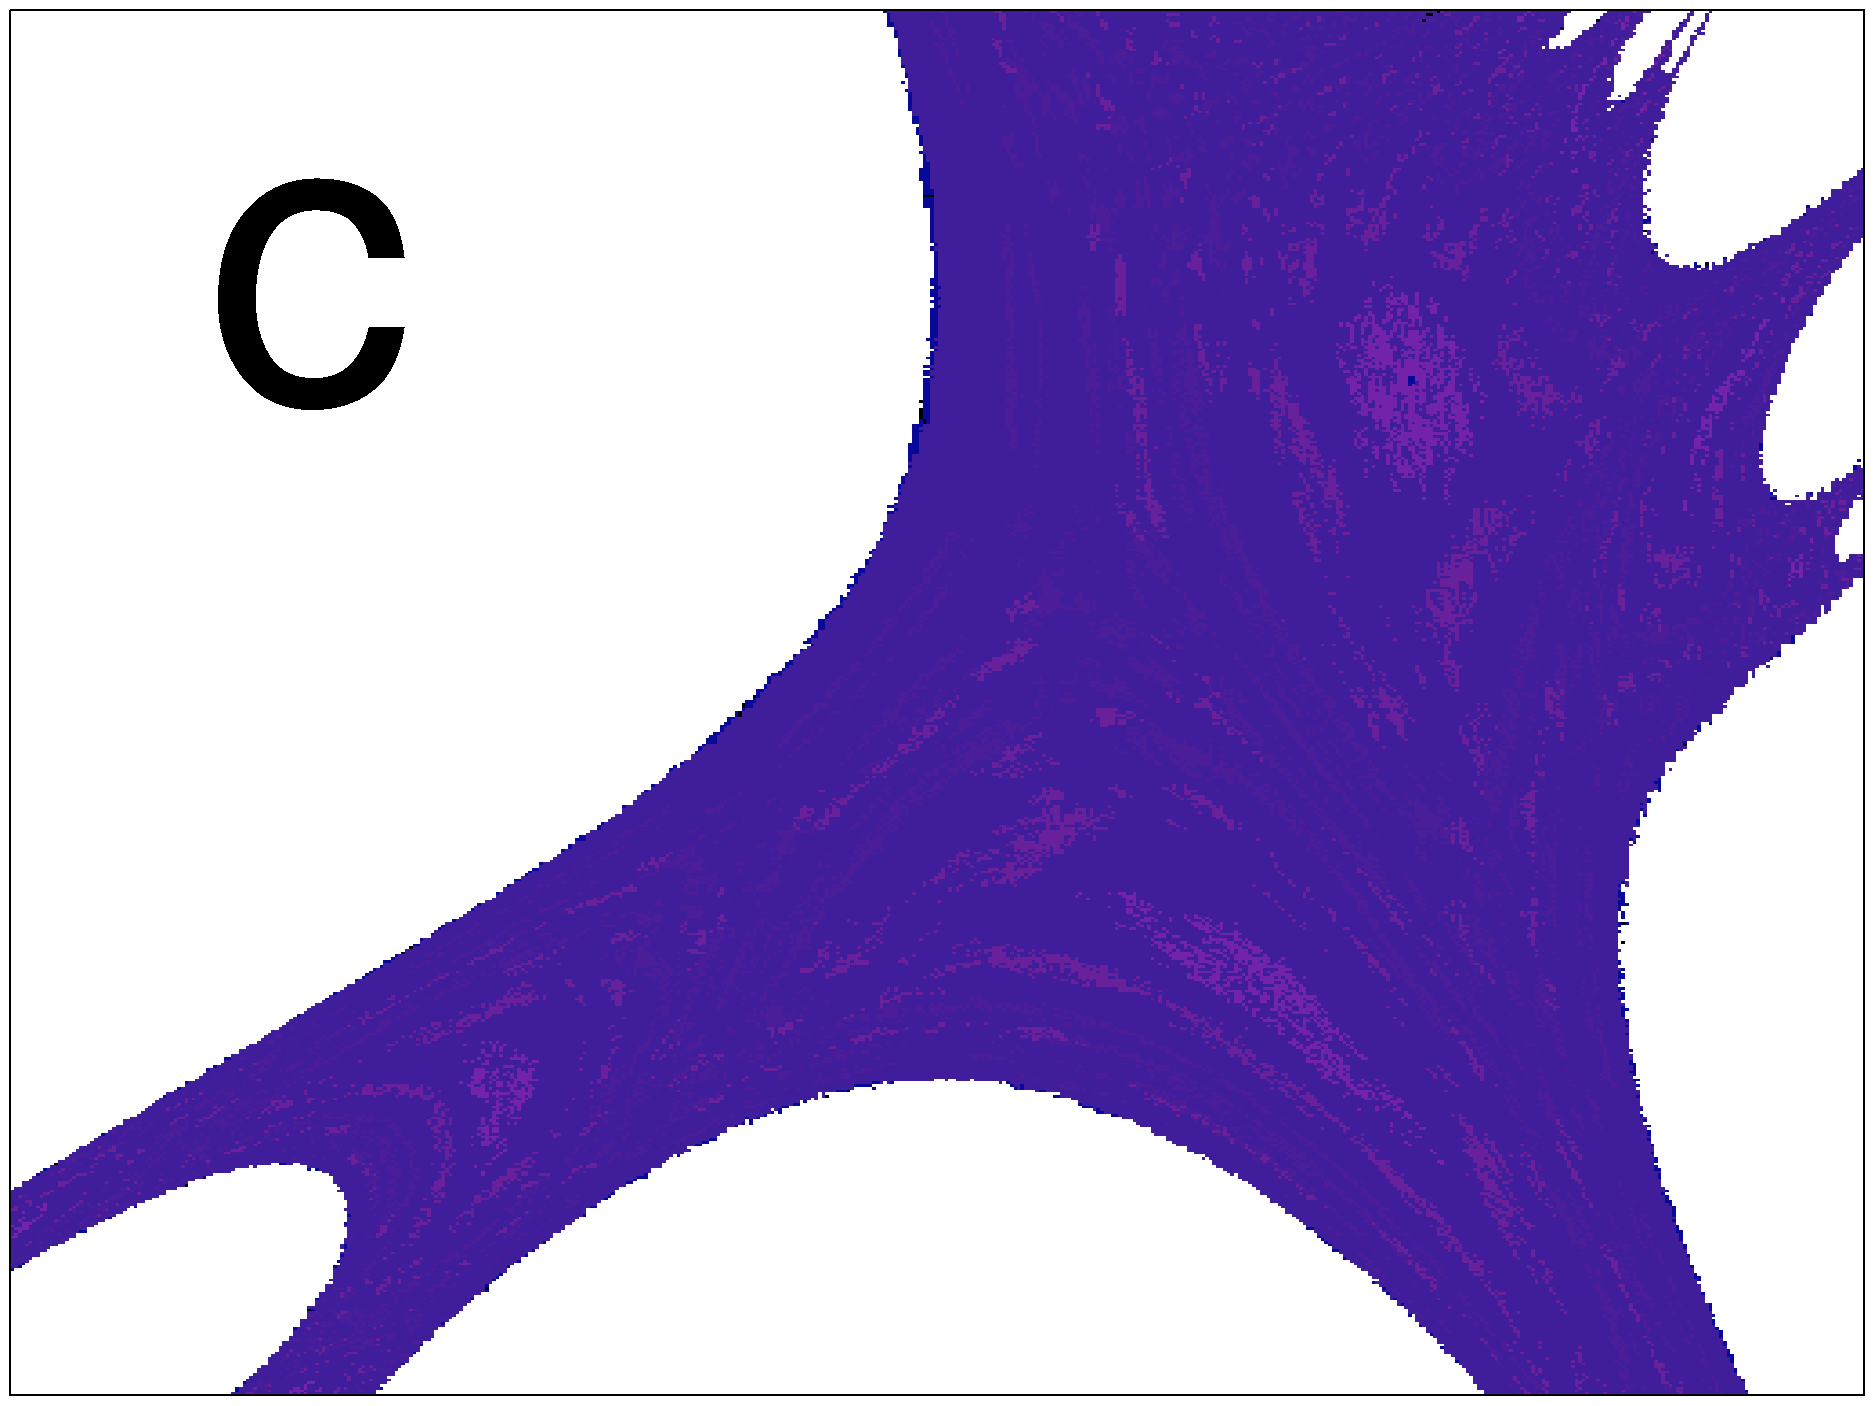
\includegraphics[width=0.3\textwidth]{m7}\\
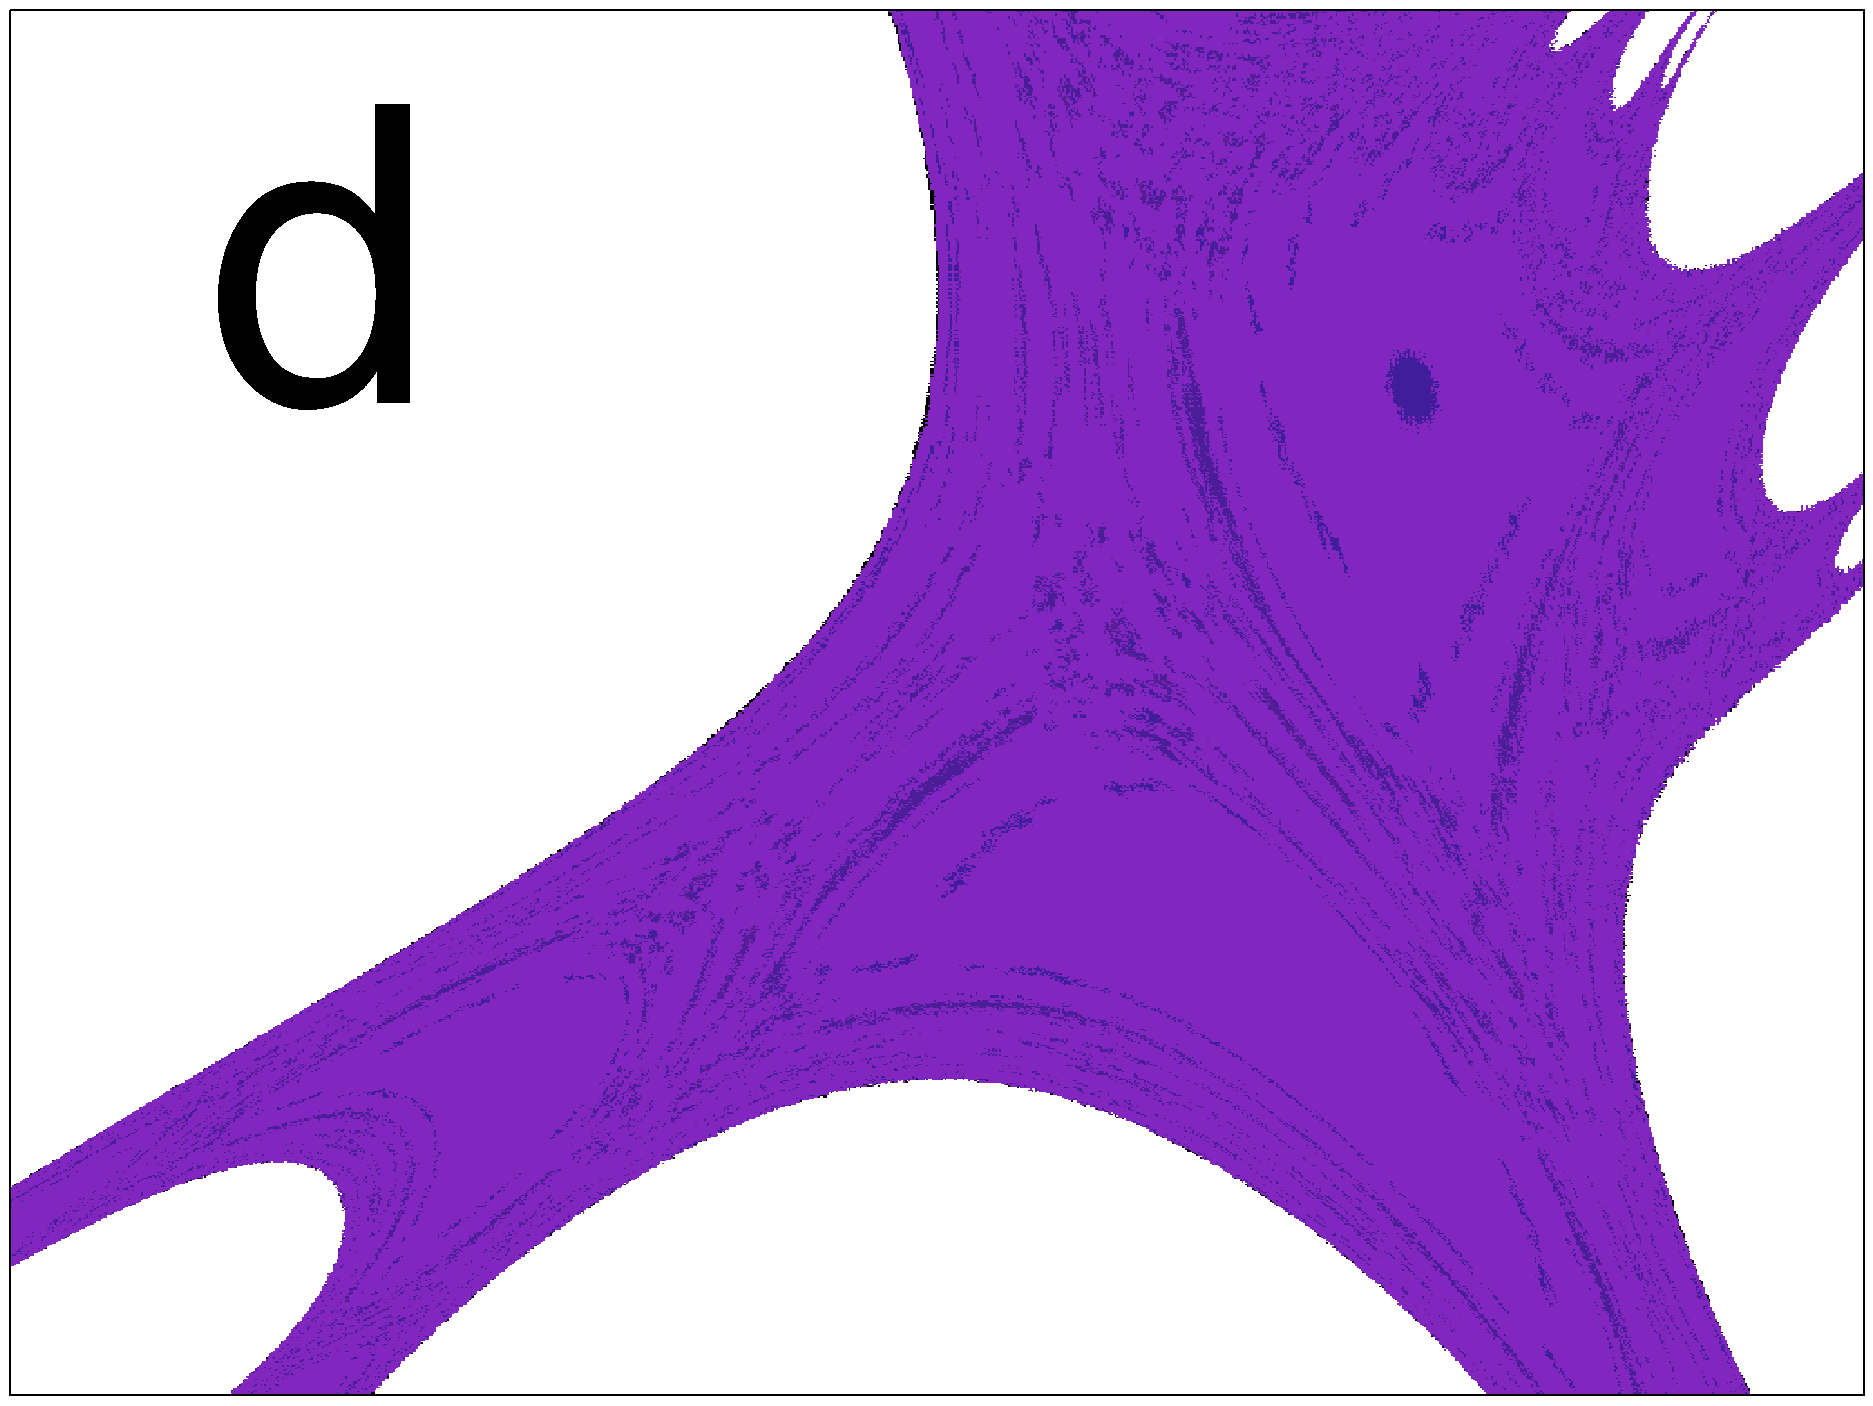
\includegraphics[width=0.3\textwidth]{m8}
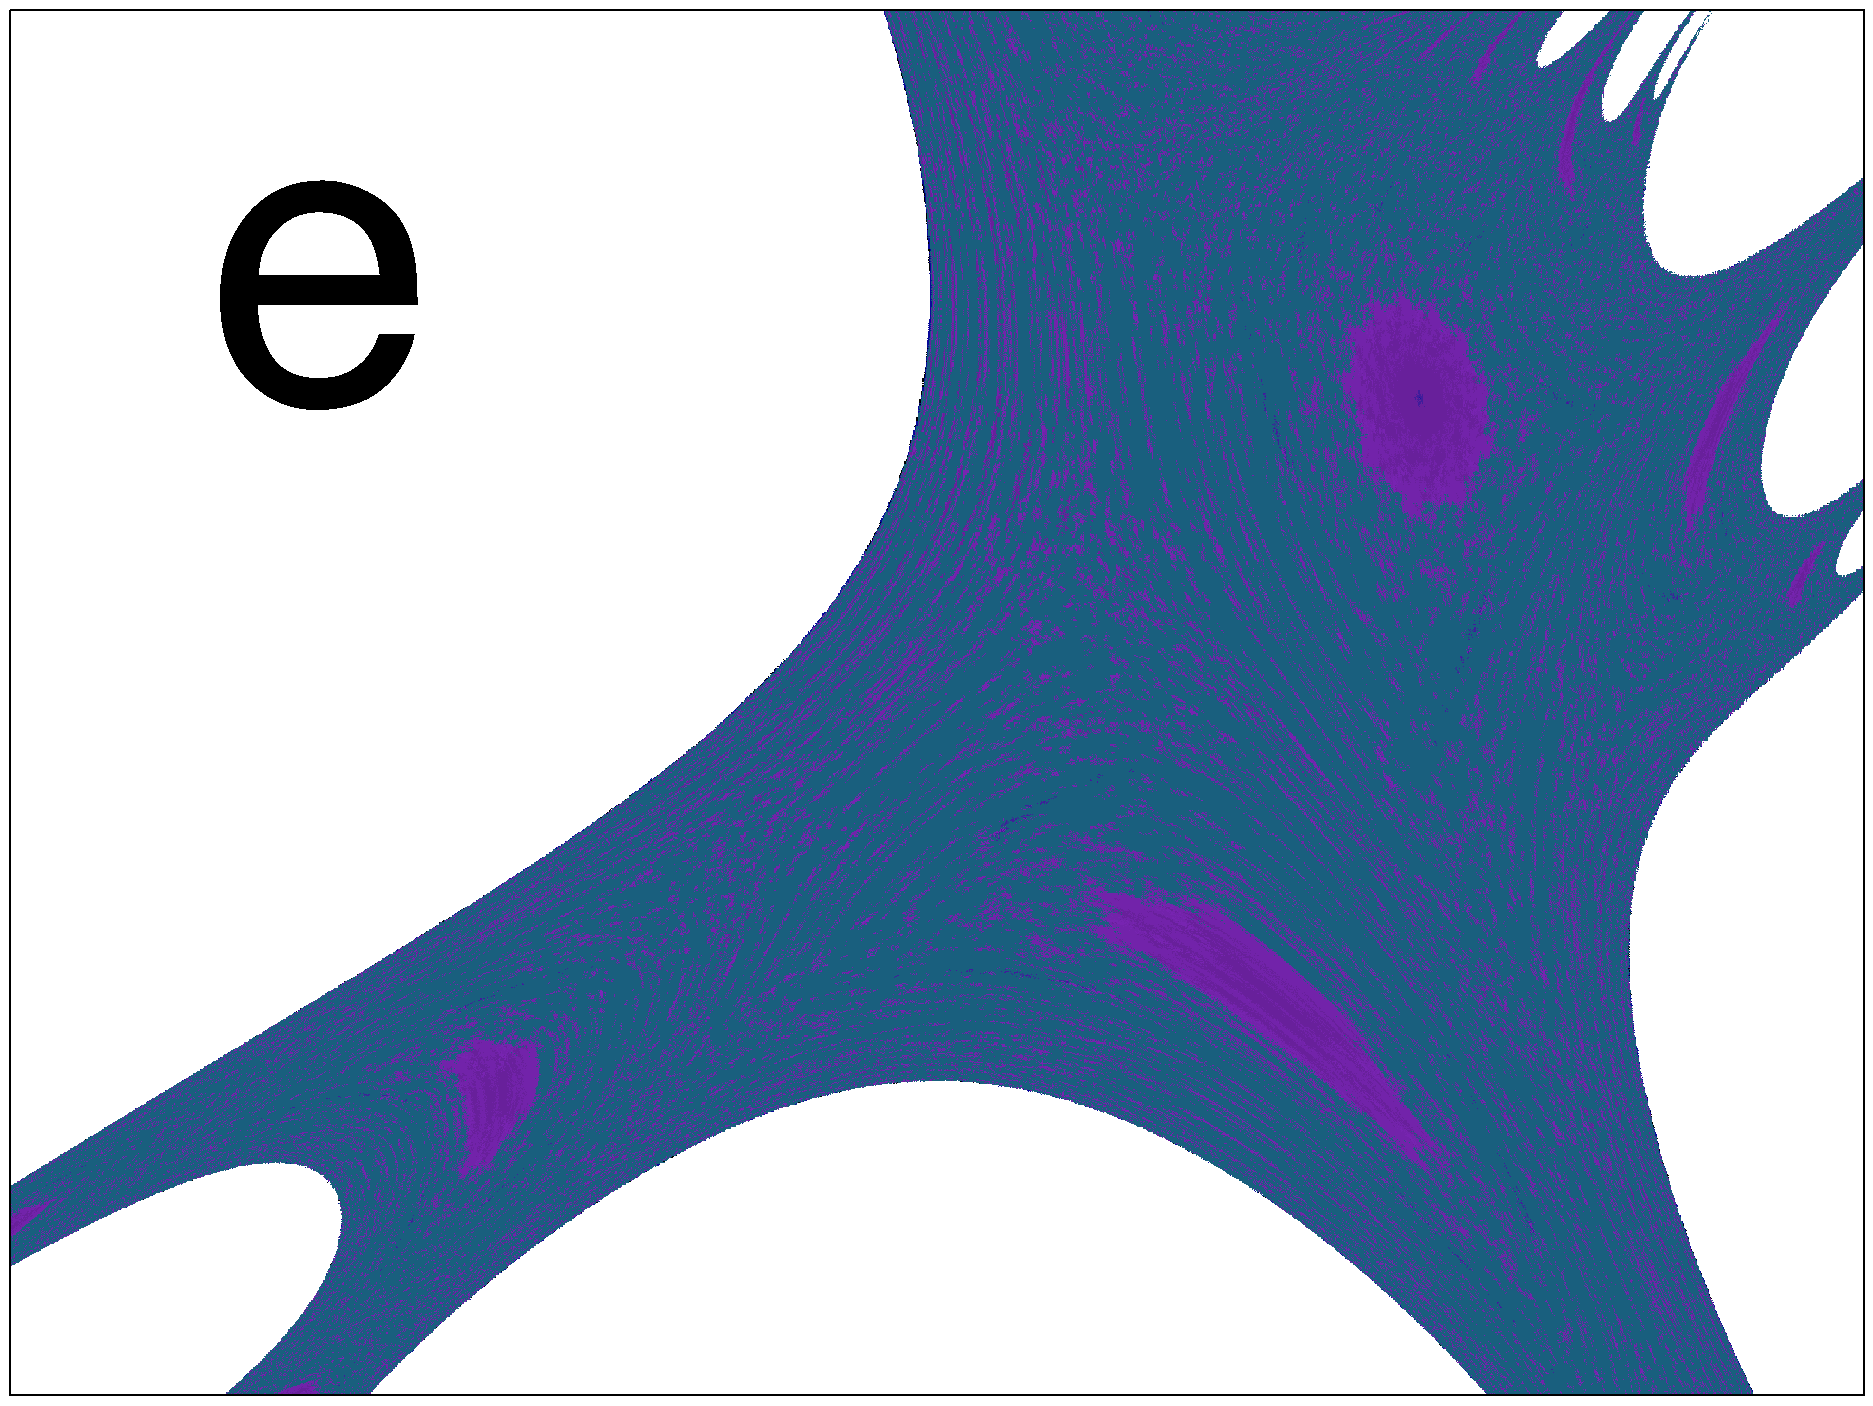
\includegraphics[width=0.3\textwidth]{m9}
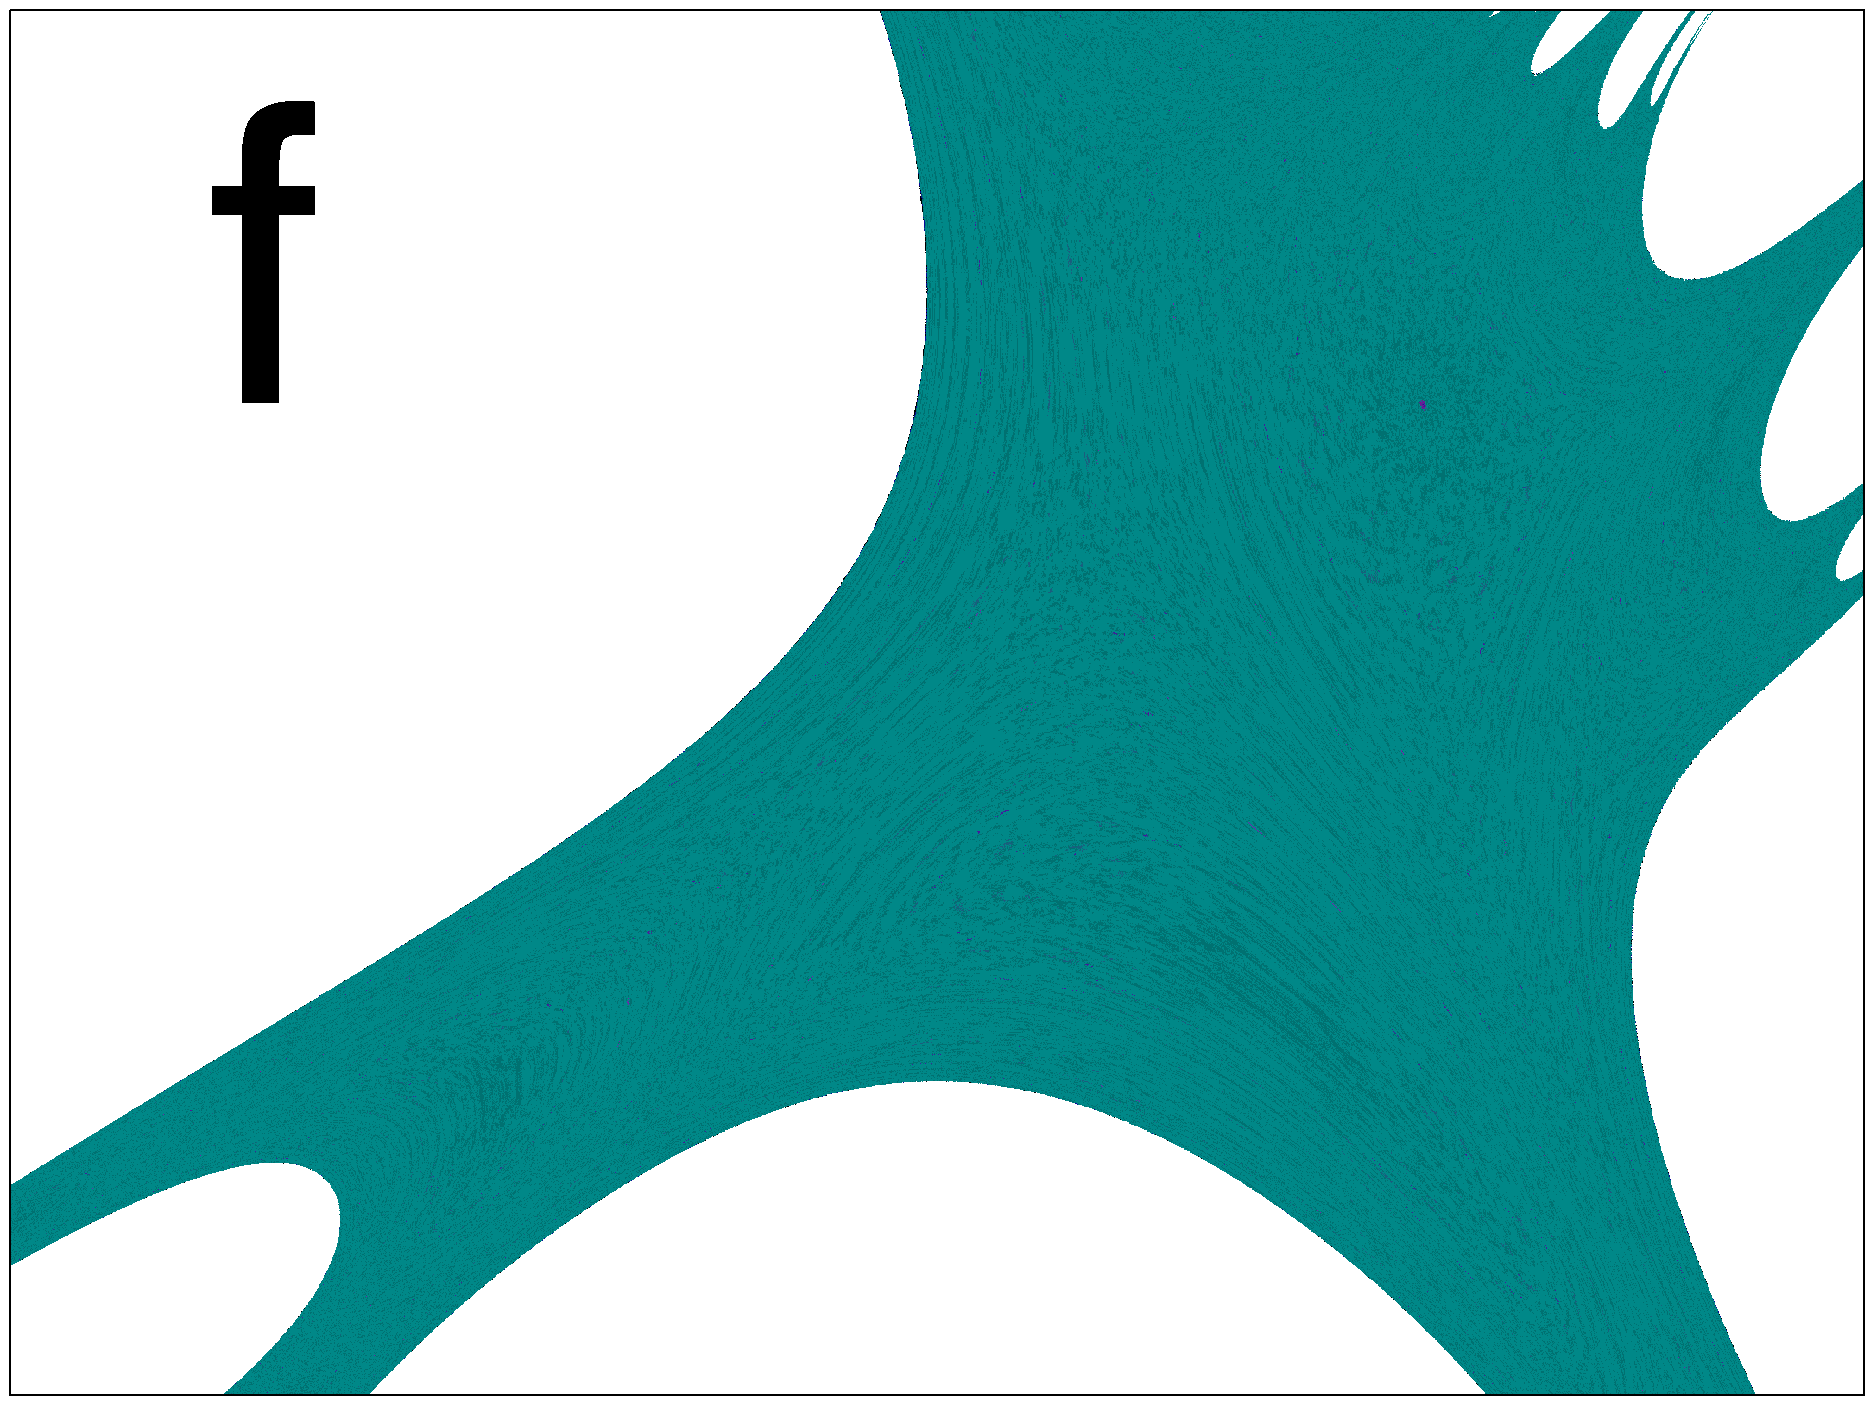
\includegraphics[width=0.3\textwidth]{m10}\\
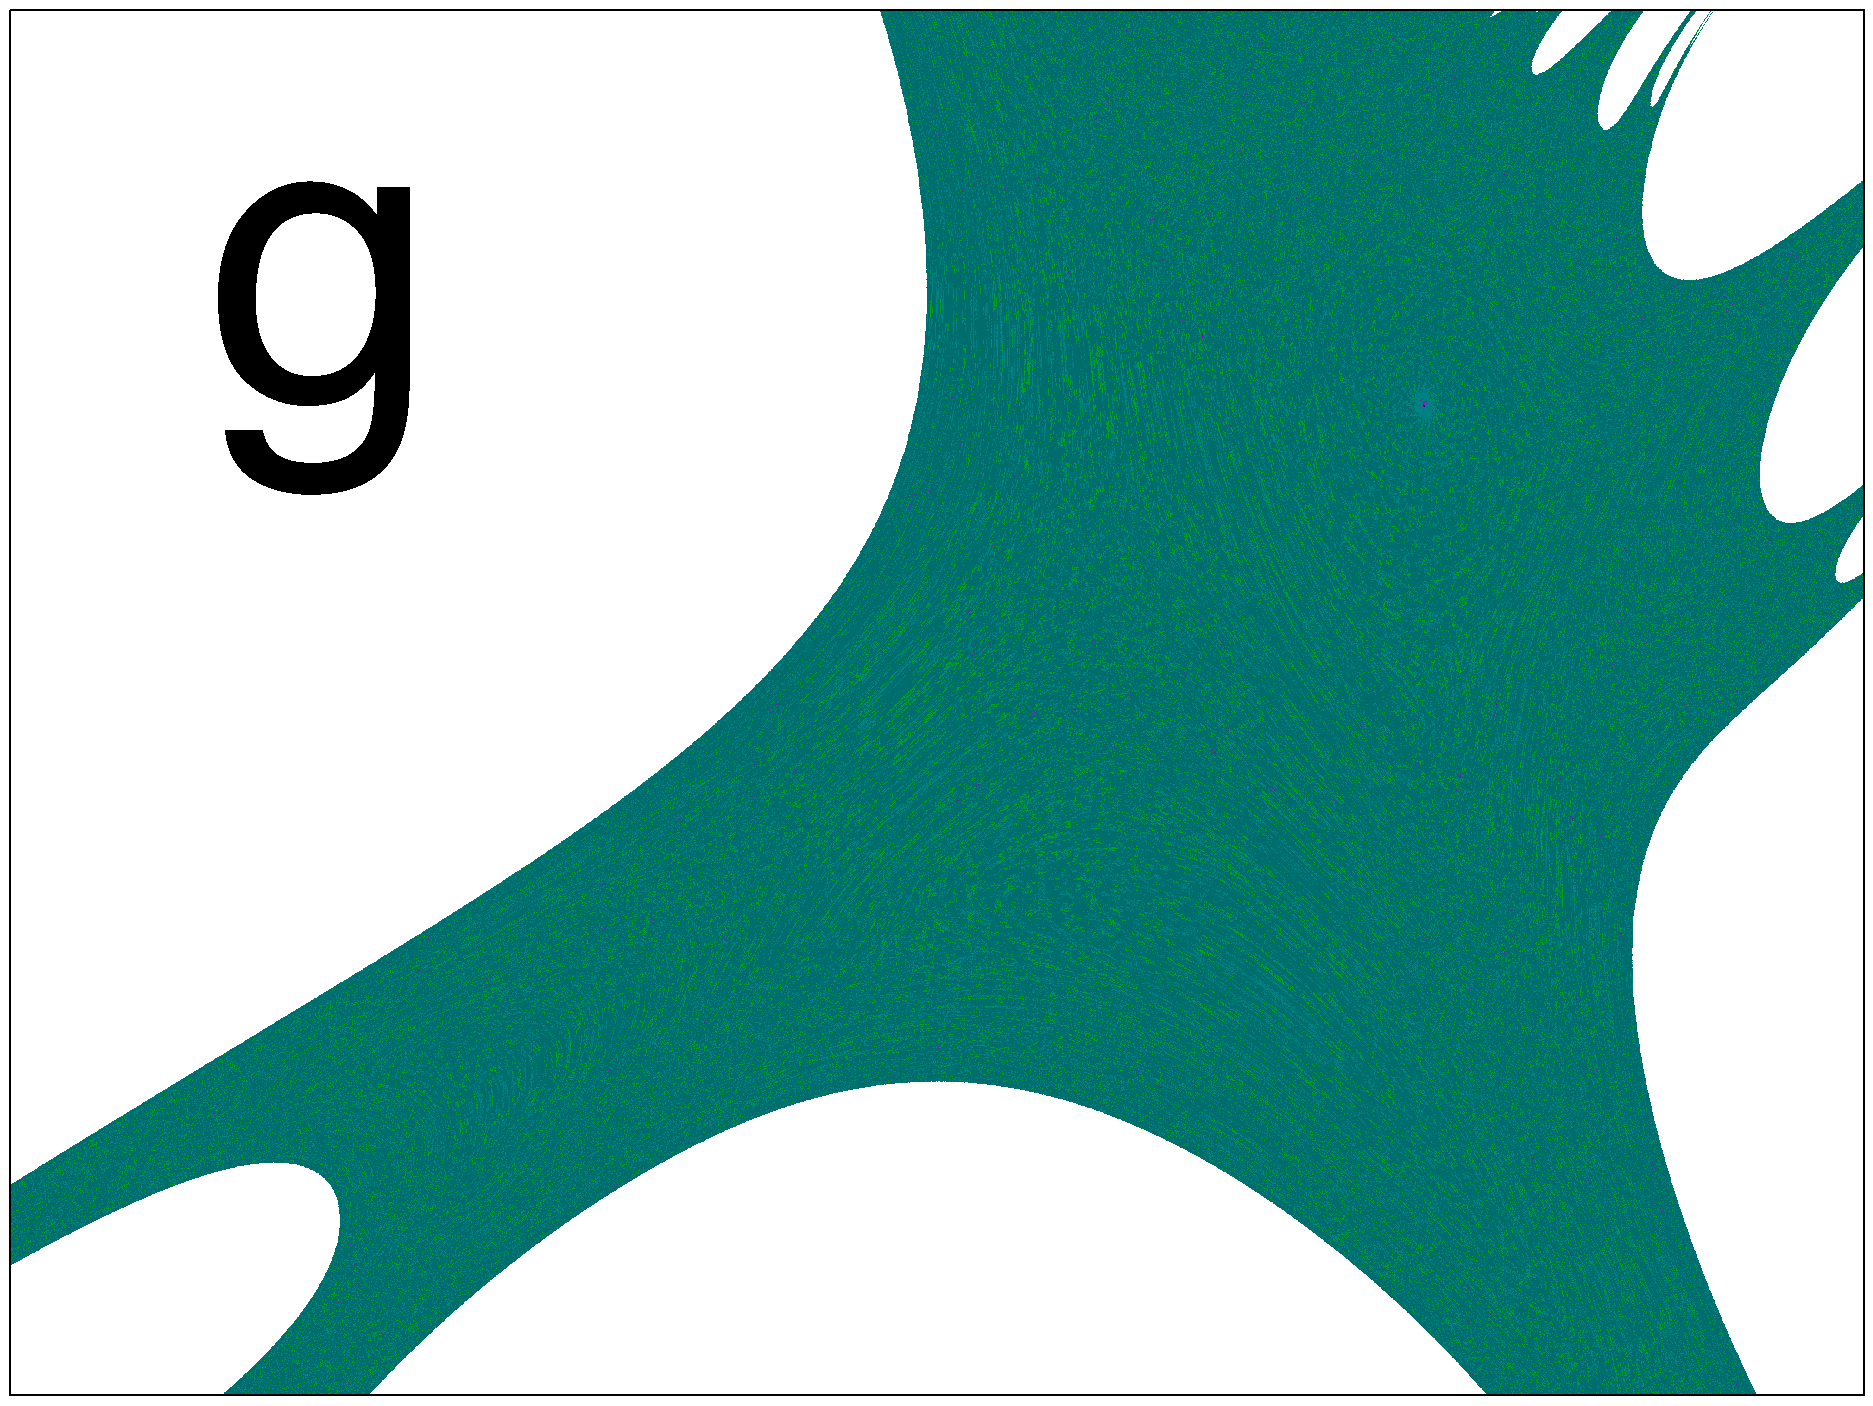
\includegraphics[width=0.3\textwidth]{m11}

\includegraphics[width=0.3\textwidth]{m12}

\includegraphics[width=0.3\textwidth]{m13}\\

\includegraphics[width=0.3\textwidth]{m14}
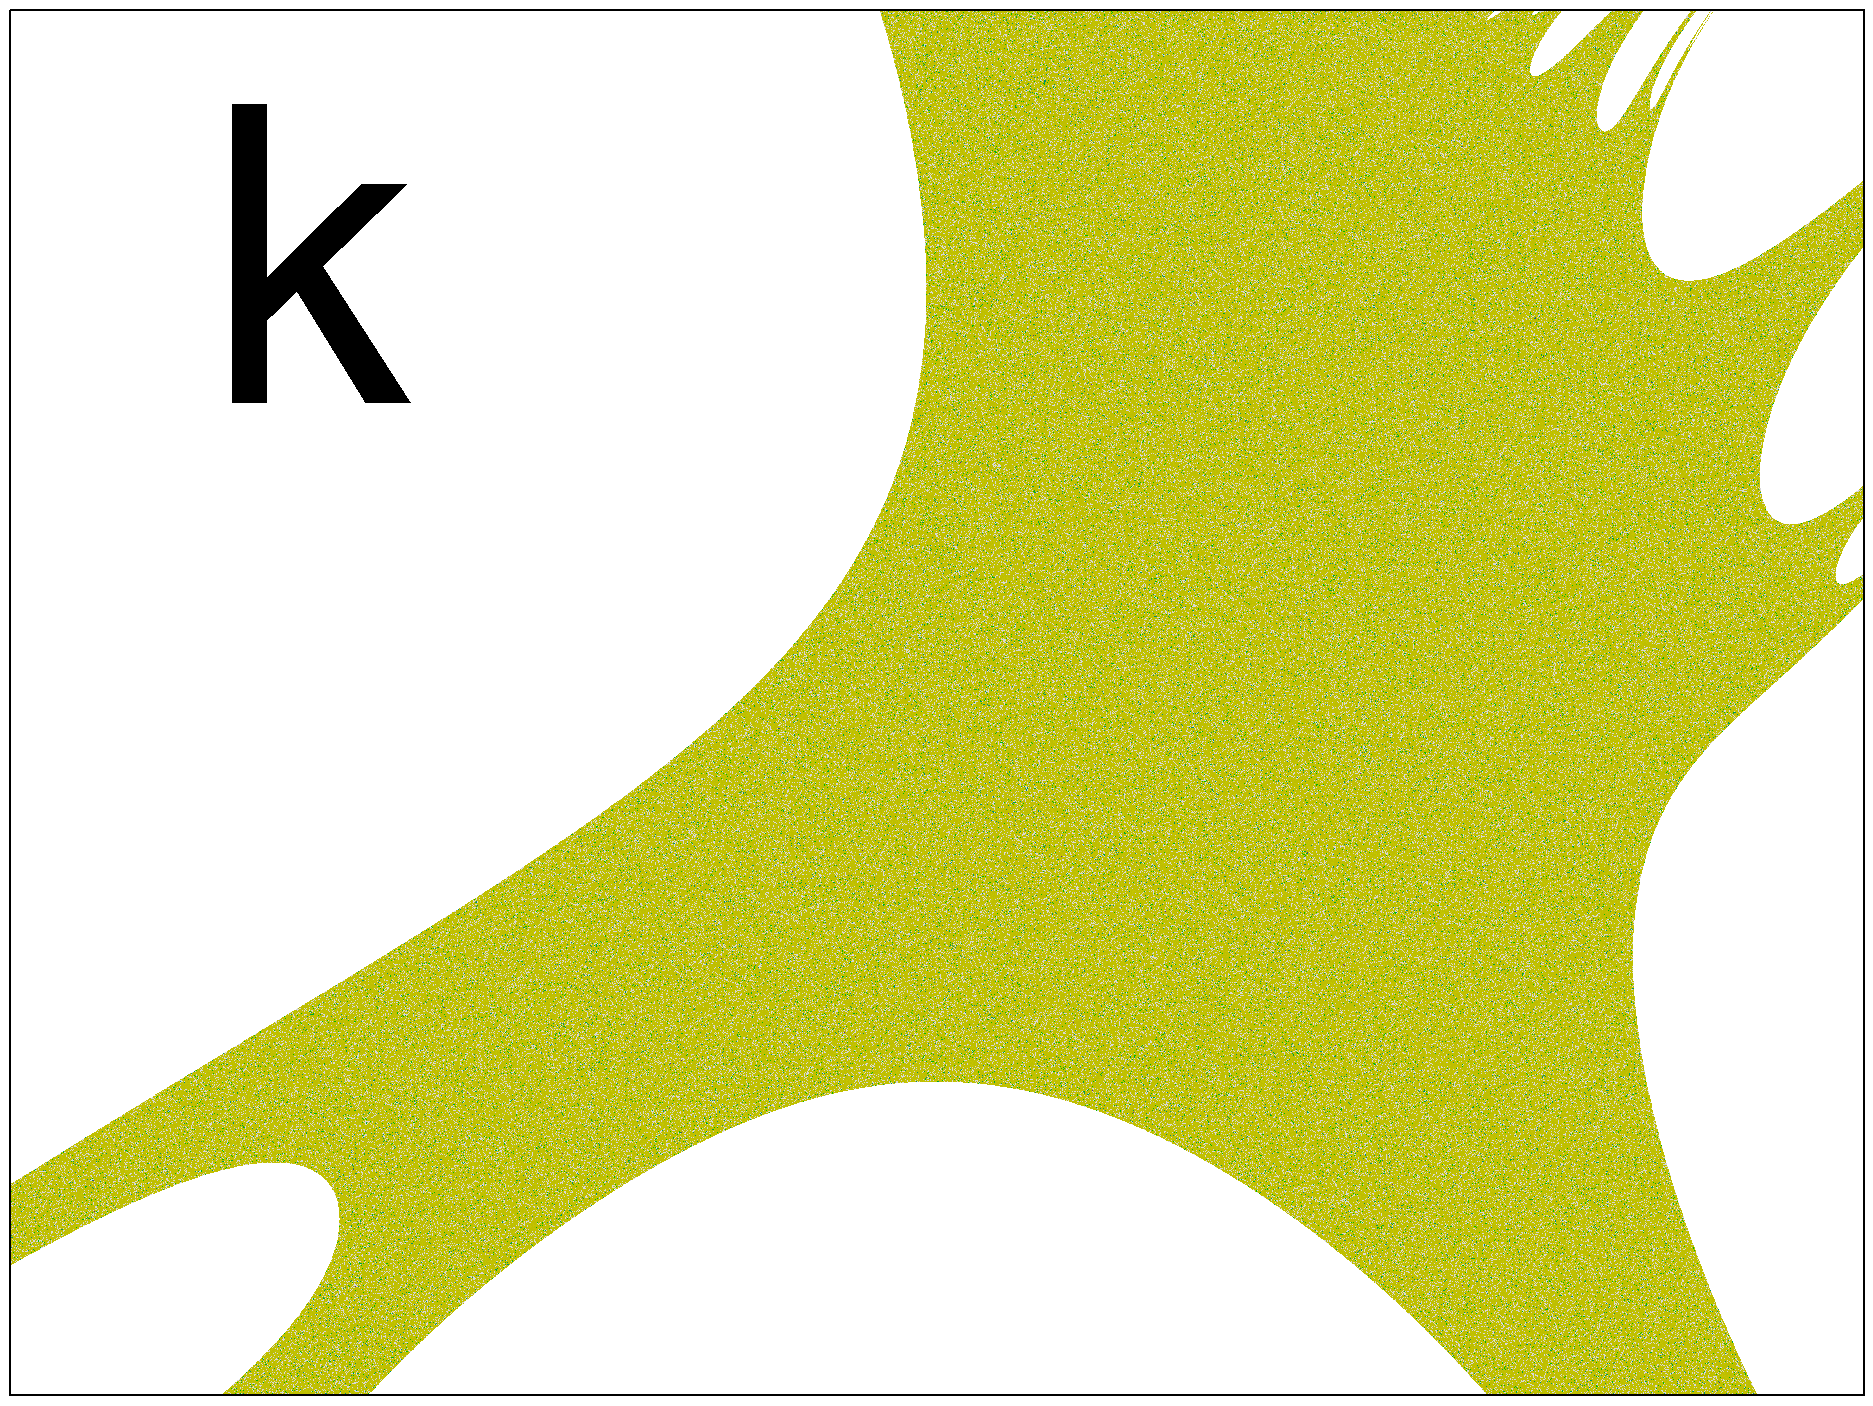
\includegraphics[width=0.3\textwidth]{m17}
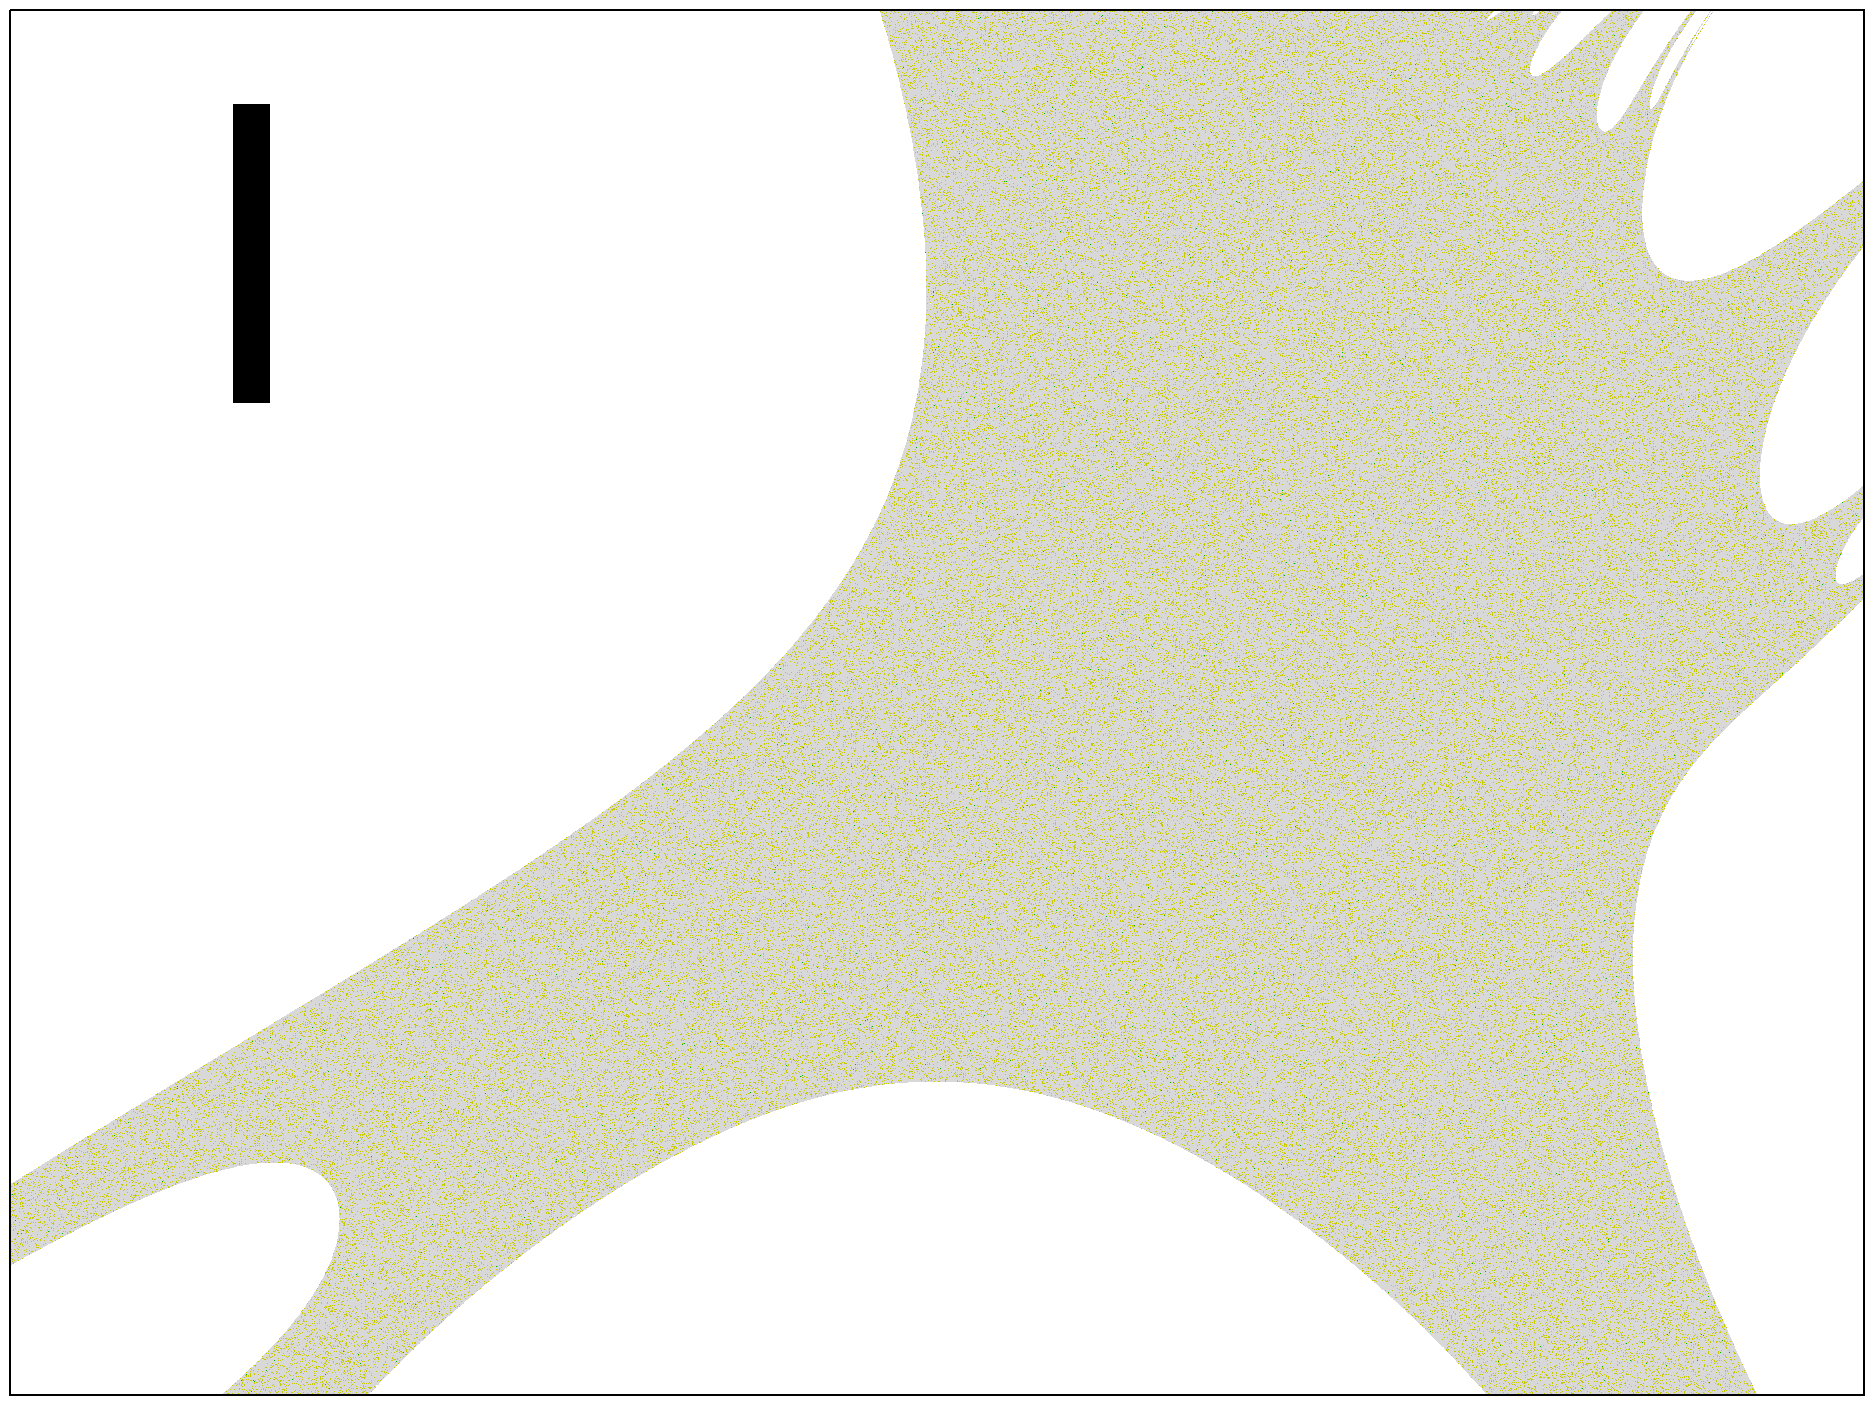
\includegraphics[width=0.3\textwidth]{m18}\\
\\   
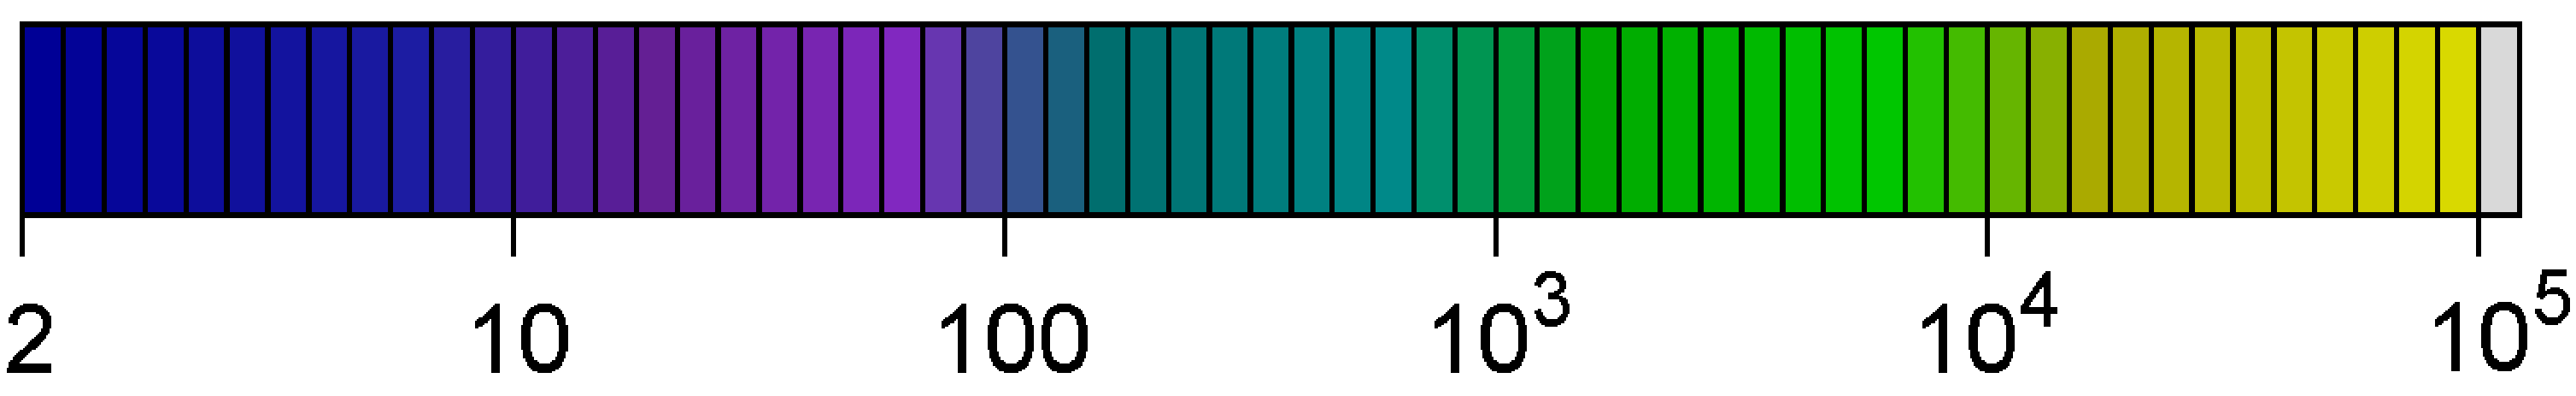
\includegraphics[width=1\textwidth]{ColorMapConEje}
\end{tabular}
\caption{Period's lengths evolution of the attraction domains for: (a) $n_f=5$, (b) $n_f=6$, (c) $n_f=7$, (d) $n_f=8$, (e) $n_f=9$, (f) $n_f=10$, (g) $n_f=11$, (h) $n_f=12$, (i) $n_f=13$, (j) $n_f=14$, (k) $n_f=17$, (l) $n_f=18$.}
\label{fig:m}
\end{figure}

Fig. \ref{fig:m} shows that as the value of $n_f$ increases the colour of the areas smooth and tend to become lighter, indicating that the CIs converge to
higher periods cycles. This is, the range of initial values
that generate useful sequences increases for higher values of $n_f$.

This can also be seen in Table \ref{tabla}, where as $n_f$ increases the predominant limit cycle's length increases. In the limit, when using floating-point architecture, that is the closest arithmetic to real numbers, all the limit cycles are higher than $10^5$, they converge to the chaotic attractor seen in Fig. \ref{fig:atractores3592}.d.

\begin{table}[!t]
% increase table row spacing, adjust to taste
\renewcommand{\arraystretch}{1.3}

\caption{Lengths of the periods within the attractor domain $x$ and $y$ $\epsilon$  $[-2,2]$.}
\label{tabla}
\centering
% Some packages, such as MDW tools, offer better commands for making tables
% than the plain LaTeX2e tabular which is used here.
\fontsize{9}{9}\selectfont
\begin{tabular}{l  l  }
\hline
$n_f$ & $T$ {\scriptsize(Percentage of ICs that converge to this period's length cycle)}  \\
\hline
\hline
$5$ & $2$ {\scriptsize($92.7\%$ )};$6$  {\scriptsize($7.3\% )$}\\
$6$ & $88$ {\scriptsize($41.6 \% )$};$44$ {\scriptsize($36.7 \% )$};$12$ {\scriptsize($13.8\% )$};$16$ {\scriptsize($6.2 \% )$};$2$ {\scriptsize($0.8 \% )$};$24$ {\scriptsize($0.6 \% )$};$26$ {\scriptsize($0.2 \%)$}\\
$7$ &  $12$ {\scriptsize($83.5 \% )$};$14$ {\scriptsize($8.9\% )$};$24$ {\scriptsize($5.2\% )$};$34$ {\scriptsize($1.8 \% )$};$2$ {\scriptsize($0.6\% )$} \\
$8$ & $68$ {\scriptsize($91.7\%)$};$14$ {\scriptsize($6.2\%)$};$12$ {\scriptsize($1.8 \%)$};$17$ {\scriptsize($0.2\% )$};$15$ {\scriptsize($0.1 \%)$}\\ 
$9$ & $140$ {\scriptsize($54.5 \%)$};$123$ {\scriptsize($25.4 \%)$};$34$ {\scriptsize($8.6\%)$};$44$ {\scriptsize($4.3 \%)$};$38$ {\scriptsize($3.9 \%)$};$22$ {\scriptsize($2.9 \%)$};$48$;$2$;$12$;$4$ {\scriptsize($<0.1\%)$}\\
$10$ & $655$ {\scriptsize($78.2\%)$};$212$ {\scriptsize($21.1\%)$};$143$ {\scriptsize($0.5\%)$};$12$ {\scriptsize($0.1\%)$};$2$;$36$;$13$;$20$;$10$;$4$ {\scriptsize($<0.1\%)$}\\
$11$ & $153$ {\scriptsize($78.1\%)$};$461$ {\scriptsize($10.8\% )$};$1381$ {\scriptsize($8.7\%)$};$434$ {\scriptsize($2.3\%)$};$18$;$30$;$53$;$32$;$34$;$10$;$2$ {\scriptsize($<0.1\% )$}\\
$12$ & $2,278$ {\scriptsize($64.4\%)$};$438$ {\scriptsize($22.4\% )$};$598$ {\scriptsize($7.6\% )$};$886$ {\scriptsize($4.7 \%)$};$12$ {\scriptsize($0.7\%)$};$87$;$2$;$42$;$23$;$32$;$10$ {\scriptsize($<0.1\% )$}\\
$13$ & $11,510$ {\scriptsize($ 98.9\%)$};$1052$ {\scriptsize($1 \%)$};$12$;$26$;$2$;$10$ {\scriptsize($<0.1\% )$}\\
$14$ & $21,333$ {\scriptsize($69.2\% )$};$5.804$ {\scriptsize($16.5\%  )$};$4,795$ {\scriptsize($7.9\%  )$};$1,264$ {\scriptsize($5.8 \% )$};$2,429$ {\scriptsize($0.5\% )$}\\ 
& $46$;$23$;$21$;$10$;$12$;$17$ {\scriptsize($<0.1\%  )$}\\ 
$15$ & $10,099$ {\scriptsize($58.6 \%)$};$1.762$ {\scriptsize($19.4 \%)$};$14,887$ {\scriptsize($18.3\%)$};$1,598$ {\scriptsize($3.4\%)$};$750$;$105$;$23$;$14$;$2$;$10$ {\scriptsize($<0.1\%)$}\\
$16$ & $54,718$ {\scriptsize($87.5\% )$};$5,017$ {\scriptsize($4.7\% )$};$>10^5$ {\scriptsize($3.7\% )$};$5,367$ {\scriptsize($2.5\% )$};$703$ {\scriptsize($0.9\% )$}\\
& $1,159$;$1,802$ {\scriptsize($0.2\% )$};$377$;$75$;$10$ {\scriptsize($<0.1\%  )$}\\  
$17$ & $37,812$ {\scriptsize($53.1\% )$};$38,456$ {\scriptsize($24.1\% )$};$>10^5$ {\scriptsize($16.0\%)$};$34,749$ {\scriptsize($3.0\% )$};$3,362$;$718$ {\scriptsize($1.5\%)$}\\
& $3,006$,$5,222$ {\scriptsize($0.1\% )$};$15$ {\scriptsize($<0.1 \%)$}\\  
$18$ & $>10^5$ {\scriptsize($87.4\%)$};$52,069$ {\scriptsize($12.5\% )$};$2,471$ {\scriptsize($0.1\% )$};$146$;$51$ {\scriptsize($<0.1 \%)$}\\
$float$ & $>10^5$ {\scriptsize($100\% )$}\\
\hline

\end{tabular}

\end{table}
\normalsize

In relation to the randomness quantifiers, we realized that the analysis performed up to this point was not
enough to fully describe the changes in the dynamic of a digitalized chaotic system. So we decided to further study the data obtained by employing some statistical quantifiers.

As said, in Fig. \ref{fig:avvelo}.a the two gray zones correspond to the initial conditions that converge to the two coexisting cycles of period two and six respectively. Then this two cycles will have a determined value of $H_{hist}$ and $H_{BP}$, $H_{hist}\mid_{T=2}=0.0625$, $H_{hist}\mid_{T=6}=0.1199$, $H_{BP}\mid_{T=2}=0.1053$ and $H_{BP}\mid_{T=6}=0.2723$. However, the reported value of these quantifiers can not be the average of both, since the frequency of occurrence of cycle two is much greater than that of cycle six (period two appears $92.7\%$ times while period six only $7.3\%$, see Table \ref{tabla}). Therefore, we have calculated the average weighting each quantifier by its frequency of occurrence.\\
Figure \ref{fig:HBPHhist} shows the weighted average of quantifiers $H_{hist}$, $H_{BP}$ and \textsl{MLE}. In the figure it can be seen that the three quantifiers tend to the value calculated using floating-point arithmetic. While $H_{BP}$ and \textsl{MLE} stabilize for $n_f \sim 12$ or $13$, $H_{hist}$ reaches the theoretical value for $n_f \sim 19$, showing that there are properties of the output sequences that only this quantifier can detect.

The $H_{hist}$ - $H_{BP}$ plane, shown in Fig. \ref{fig:HBPvsHhist}, allows a quick visualization of the behavior in terms of randomness of the system, in this plane the ``ideal" pointfrom the point of view of randomness is $(1,1)$. Here, again, the system seems to stabilize for $n_f$ higher than 12. It can be seen that while the $H_{hist}$ stabilizes close to the maximum value ($1$), the $H_{BP}$ tends to $ 0.5$, this value is characteristic of chaotic systems and is due to the structures of their attractors.

A summary of the observed analysis of these outputs can be seen in Fig. \ref{puntos}.

Fig. \ref{puntos}.a and \ref{puntos}.b show the
number of points that diverge and converge to fixed points
respectively as the value of $n_f$ increases, in both cases the
final value tends to the floating-point case. It is clear from
these figures that for $n_f \sim 12$ the system seems have stabilized. Figure
\ref{puntos}.c shows that the averaged period of cycles increases at a logarithmic rate.



%==========================Resumen periodos============================
\begin{figure}
\begin{tabular}{cc}
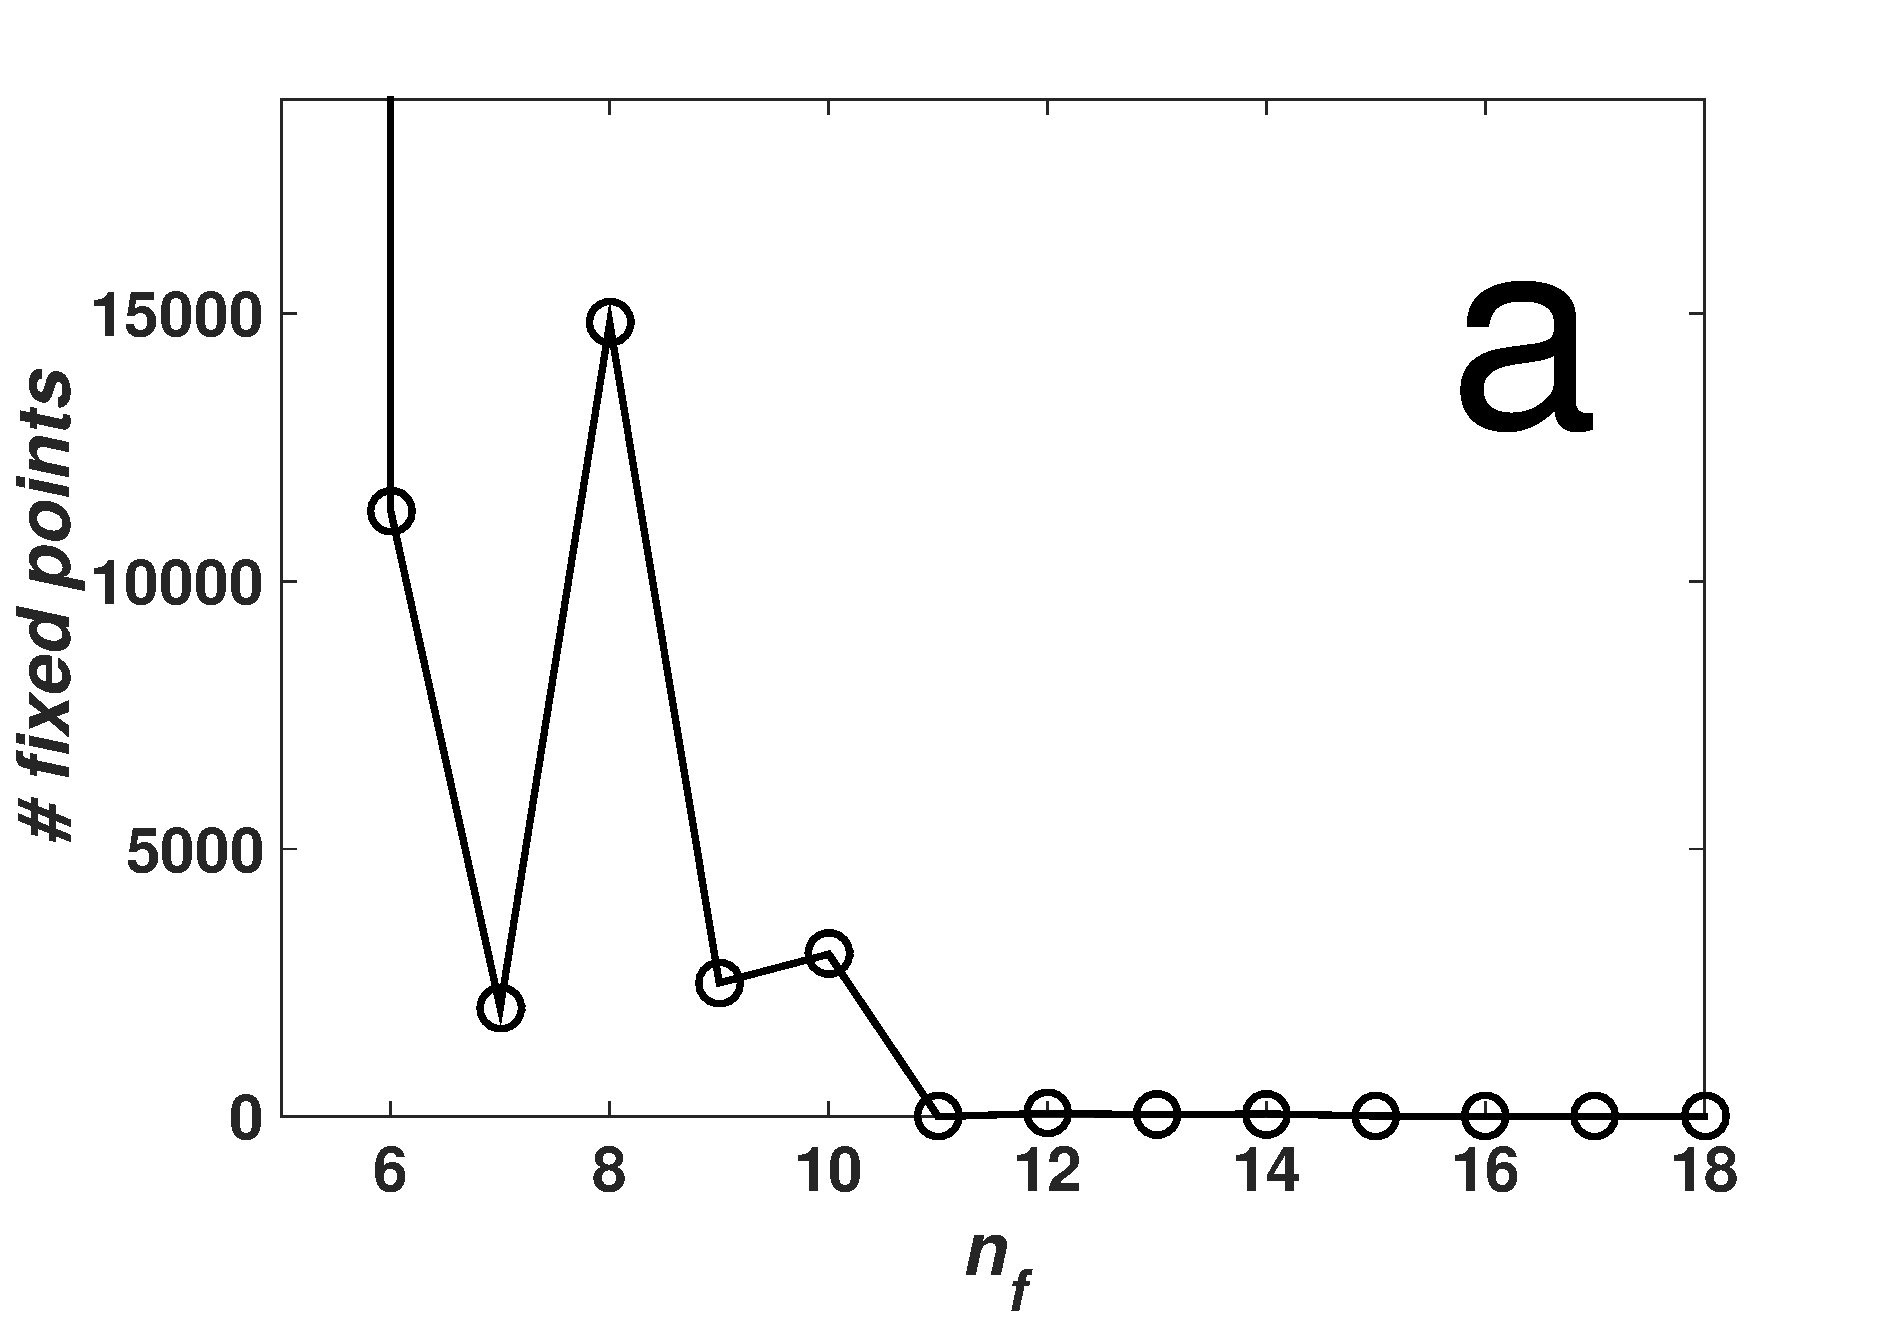
\includegraphics[width=0.48\textwidth]{ptosfijos}
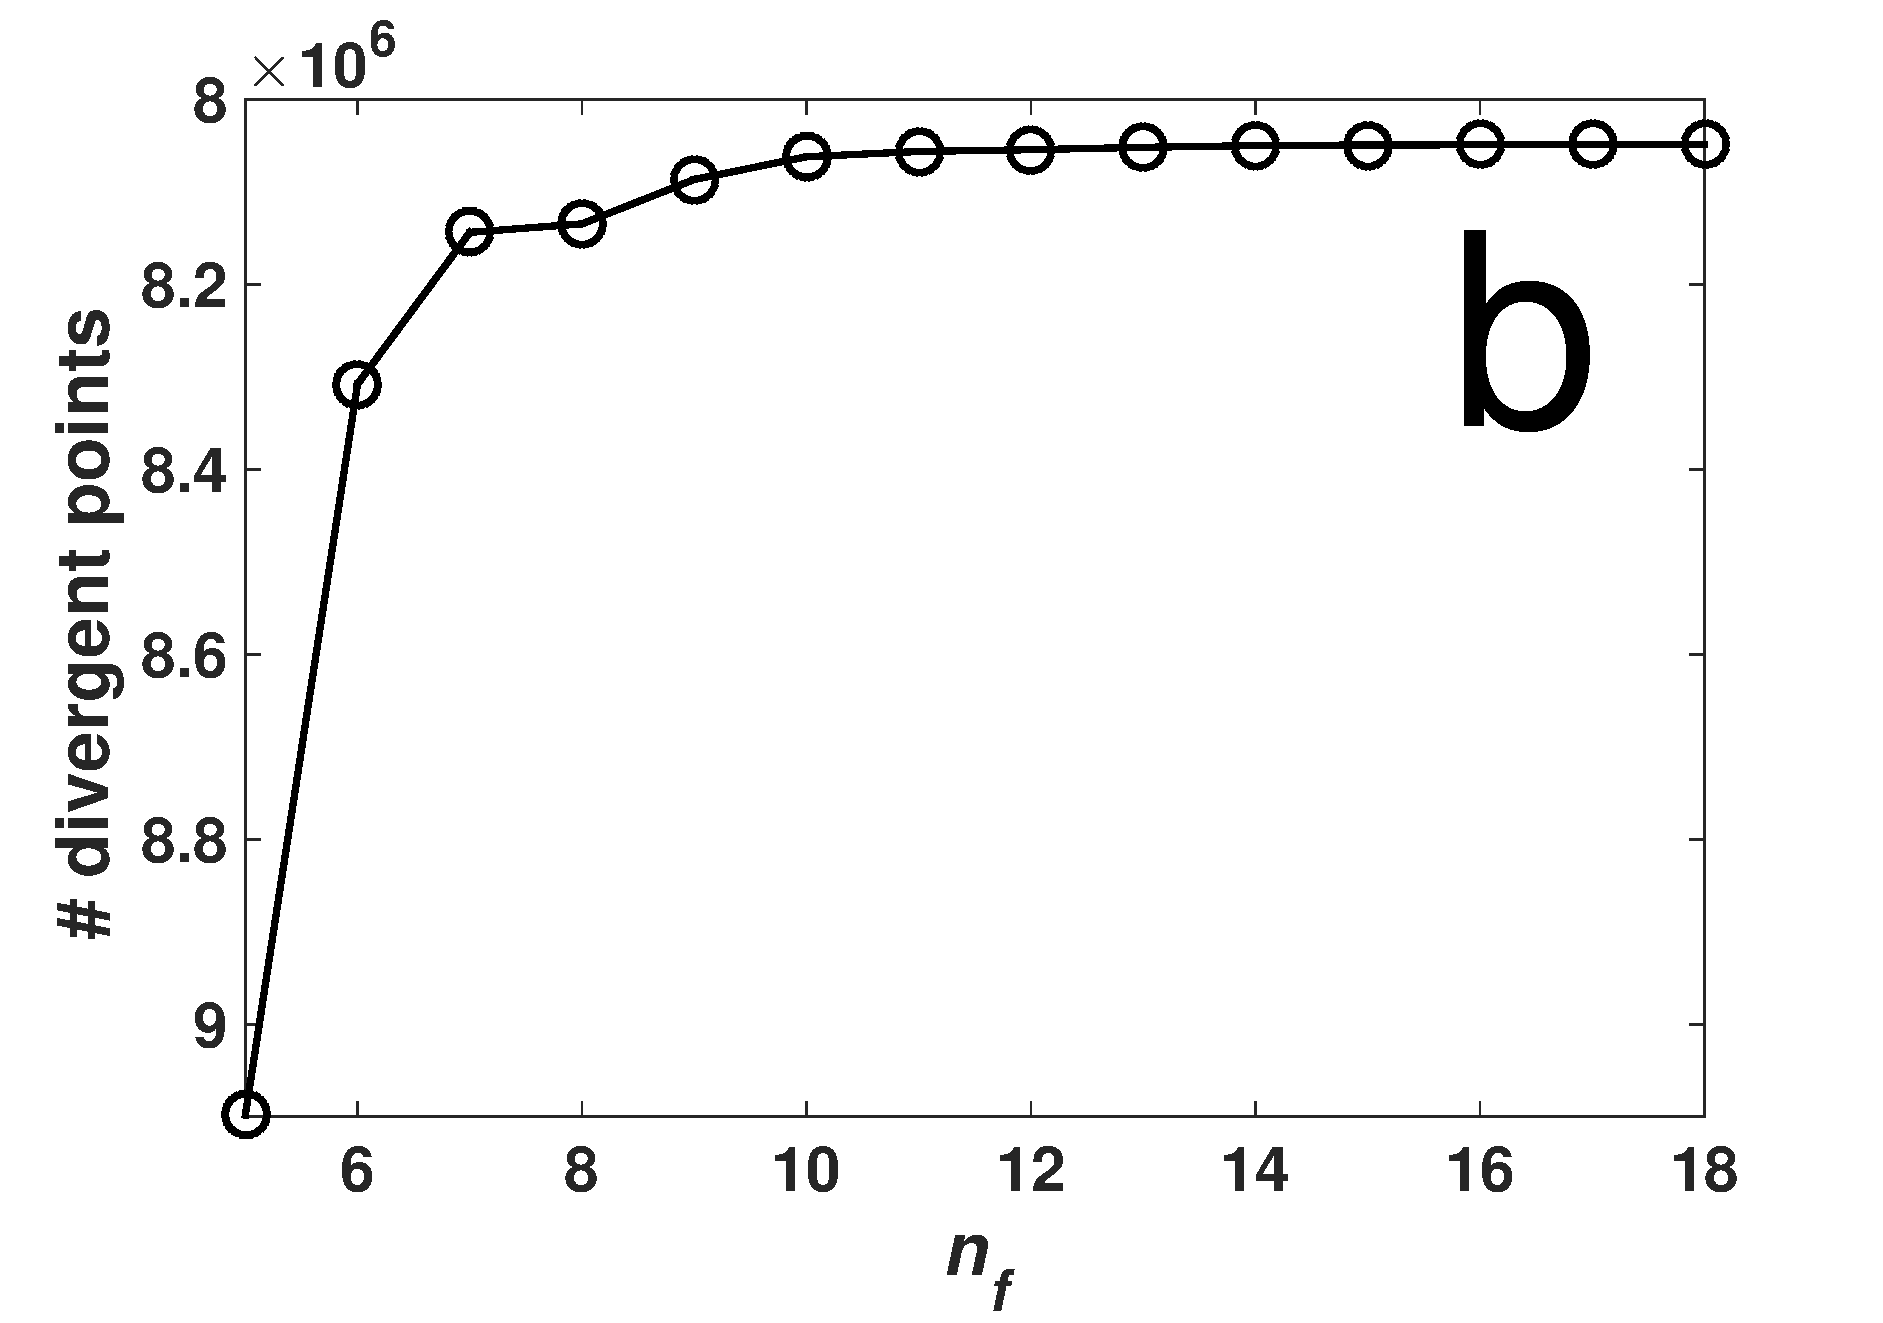
\includegraphics[width=0.48\textwidth]{divergen}\\
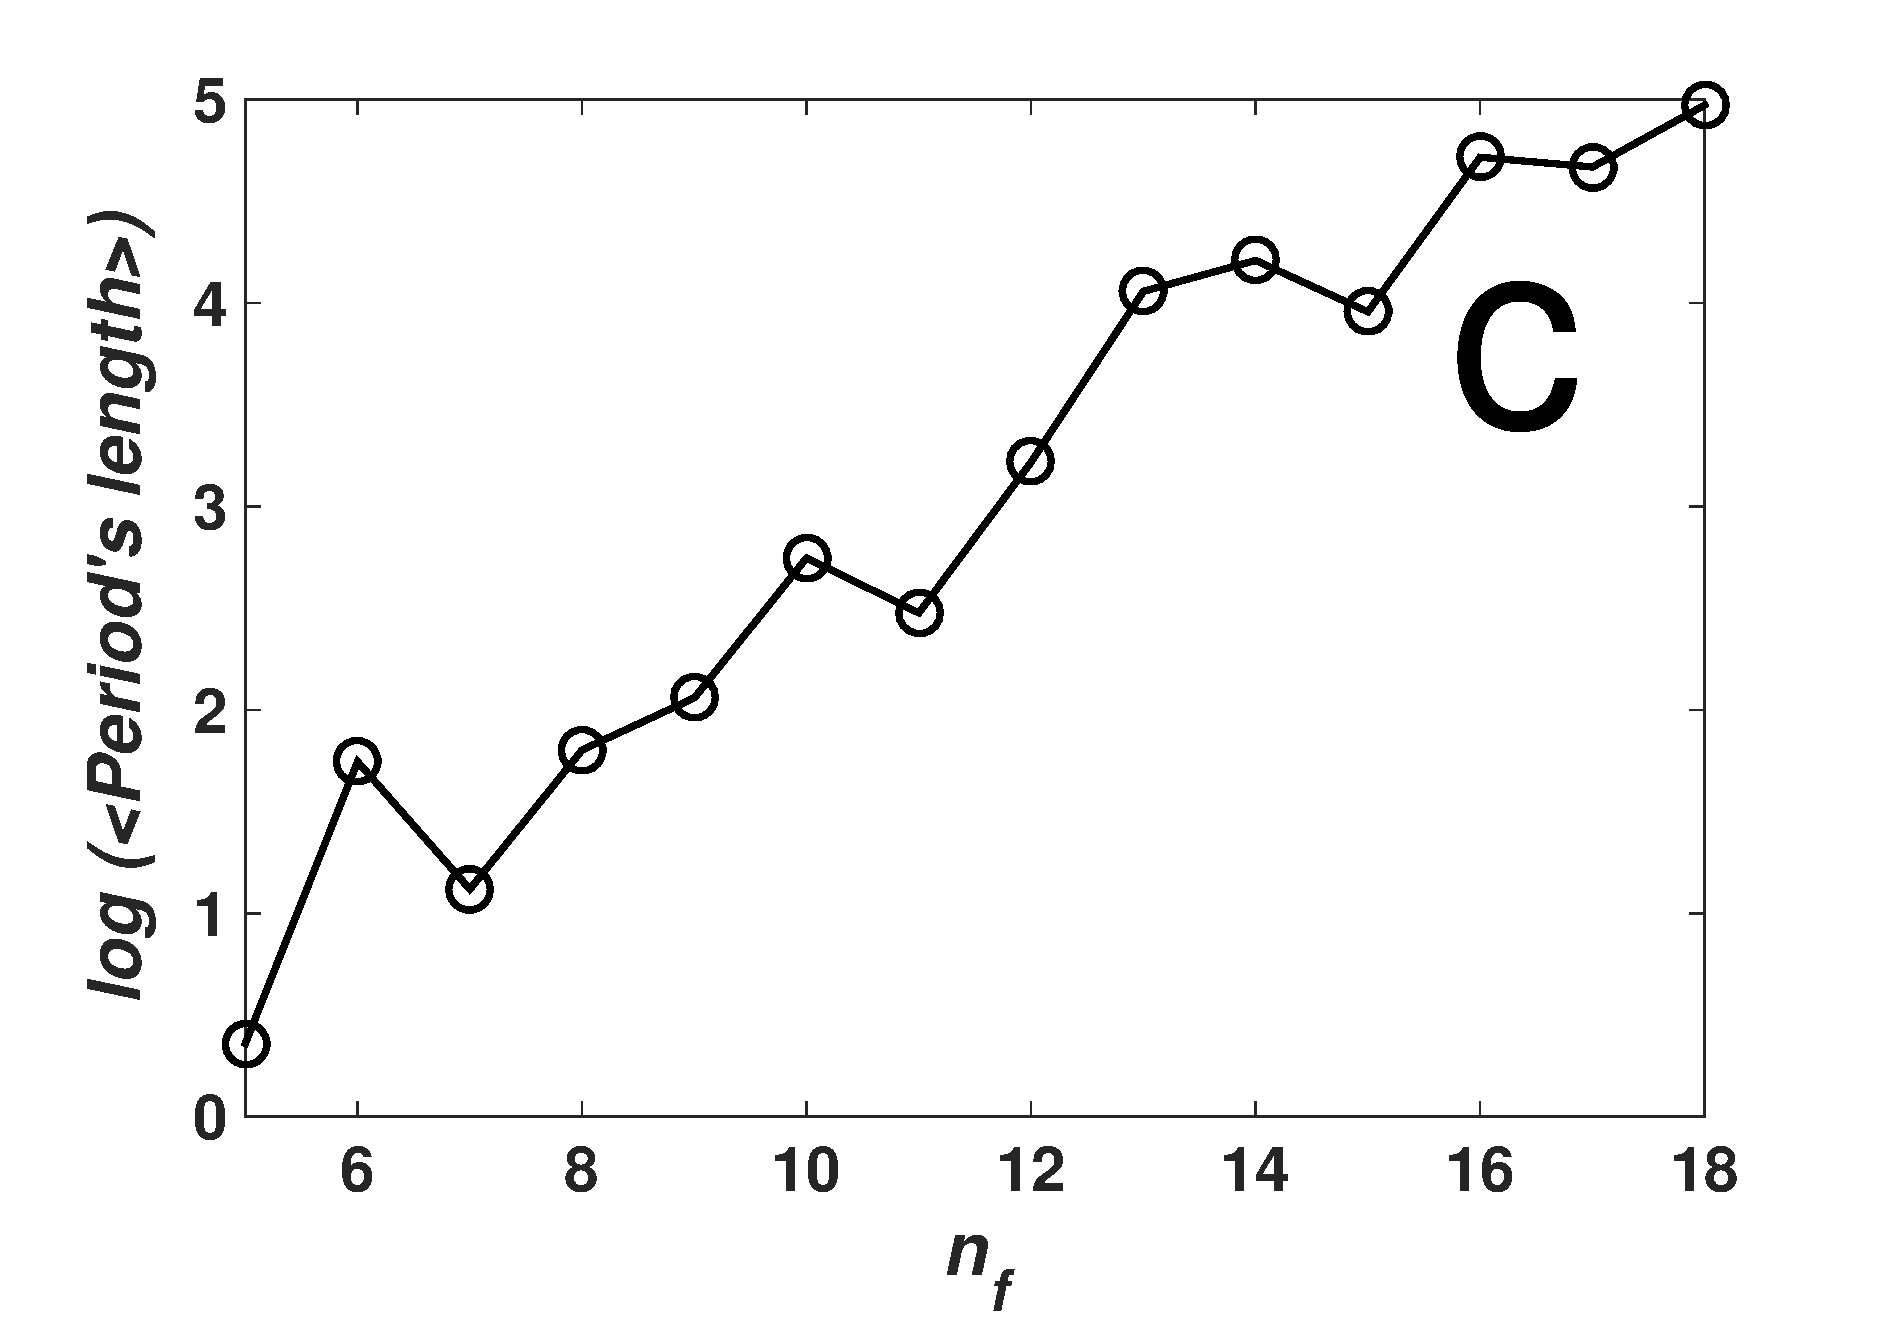
\includegraphics[width=0.48\textwidth]{Periodos_prom}
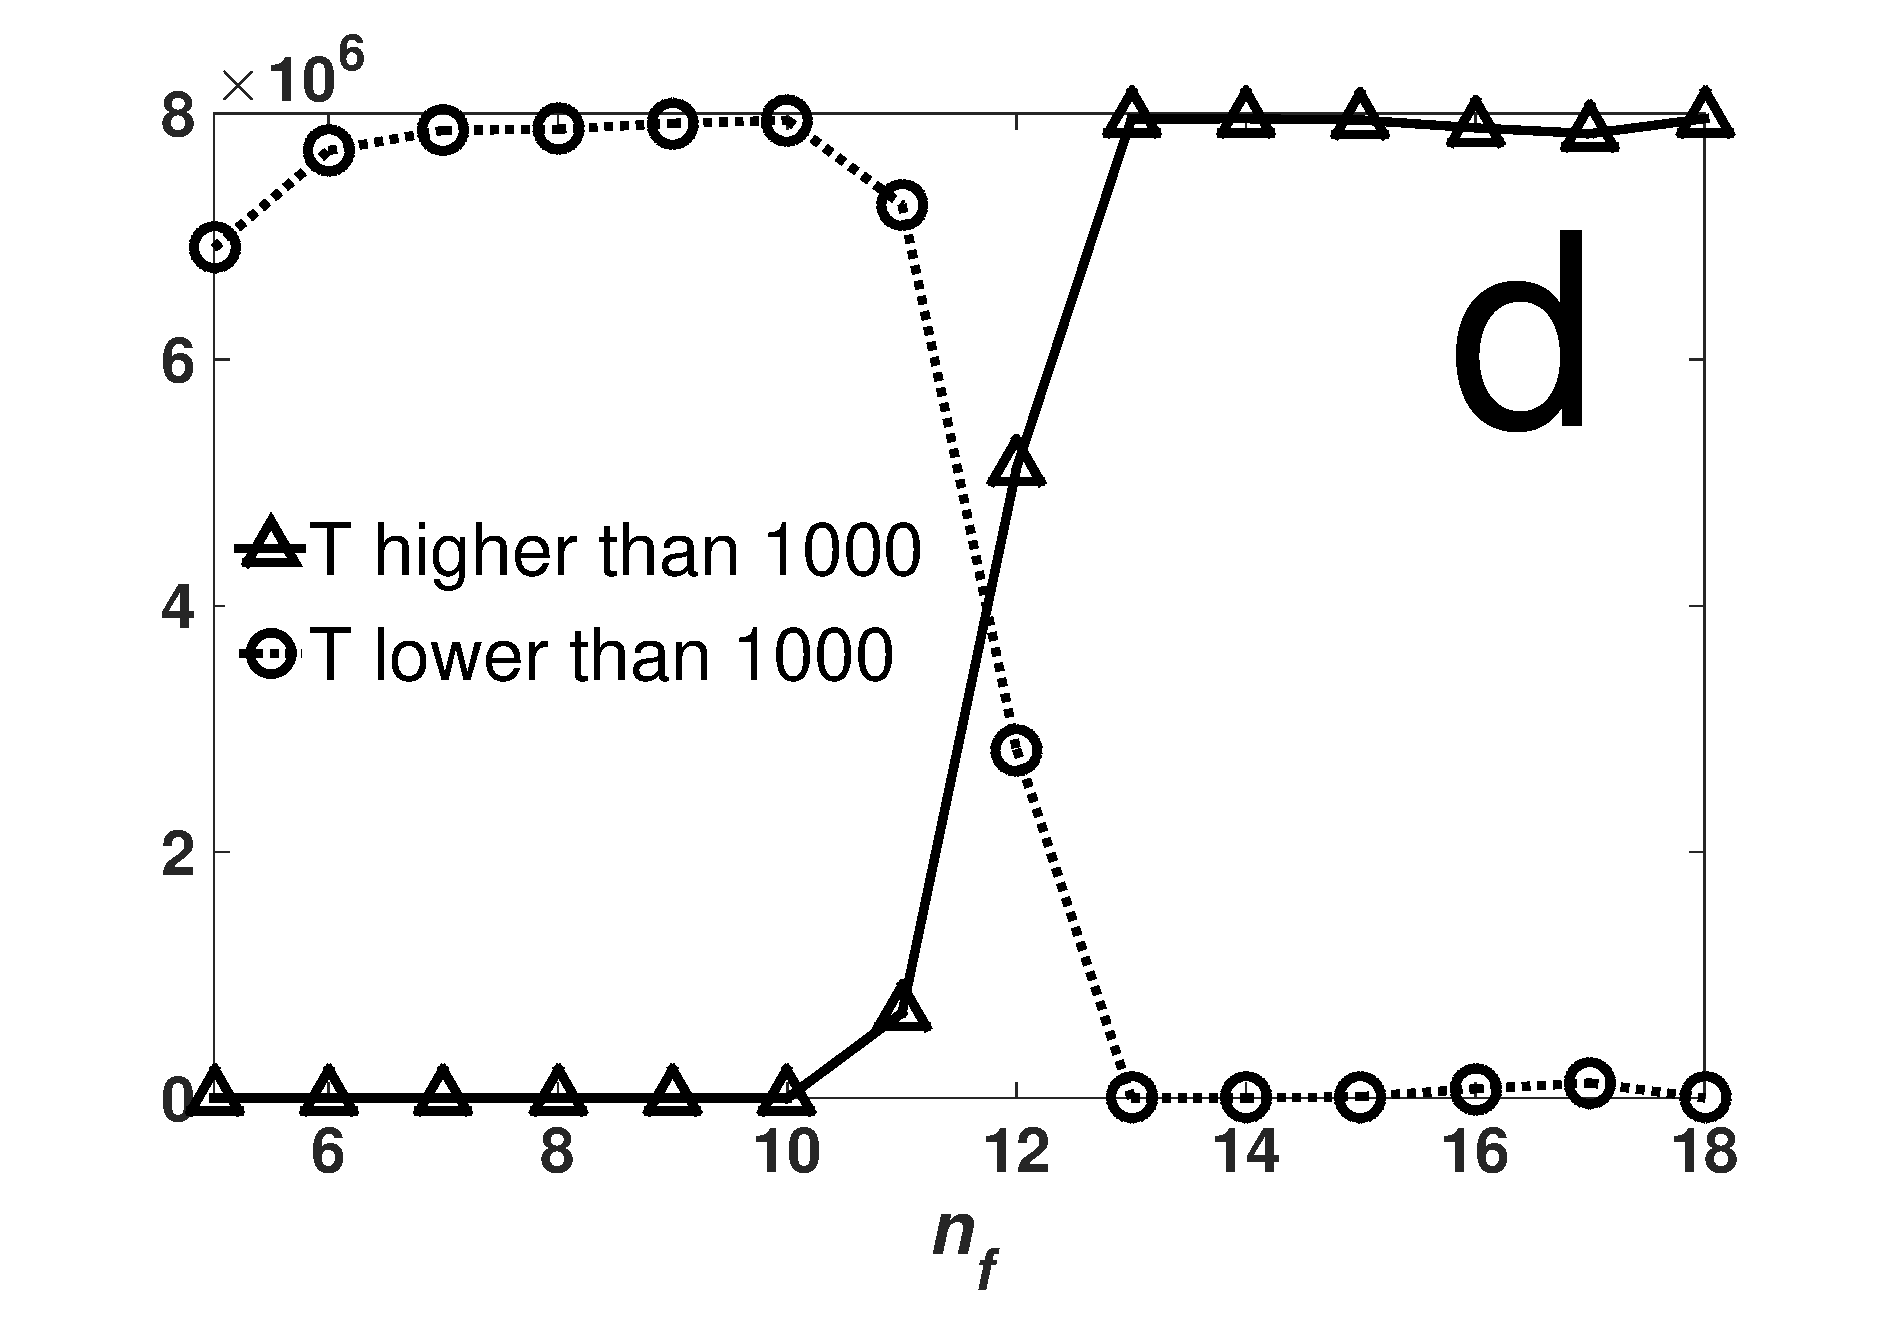
\includegraphics[width=0.48\textwidth]{Puntos}
\end{tabular}
\caption{Summary of initial conditions' behavior:
(a) number of fixed points; (b) number of divergent points; (c) logarithm of the length's cycles weighted average;  (d) initial conditions with period length higher and lower than $1,000$.}
\label{puntos}
\end{figure}
%============================================================================================
%==================================================
\begin{figure}
    \centering
        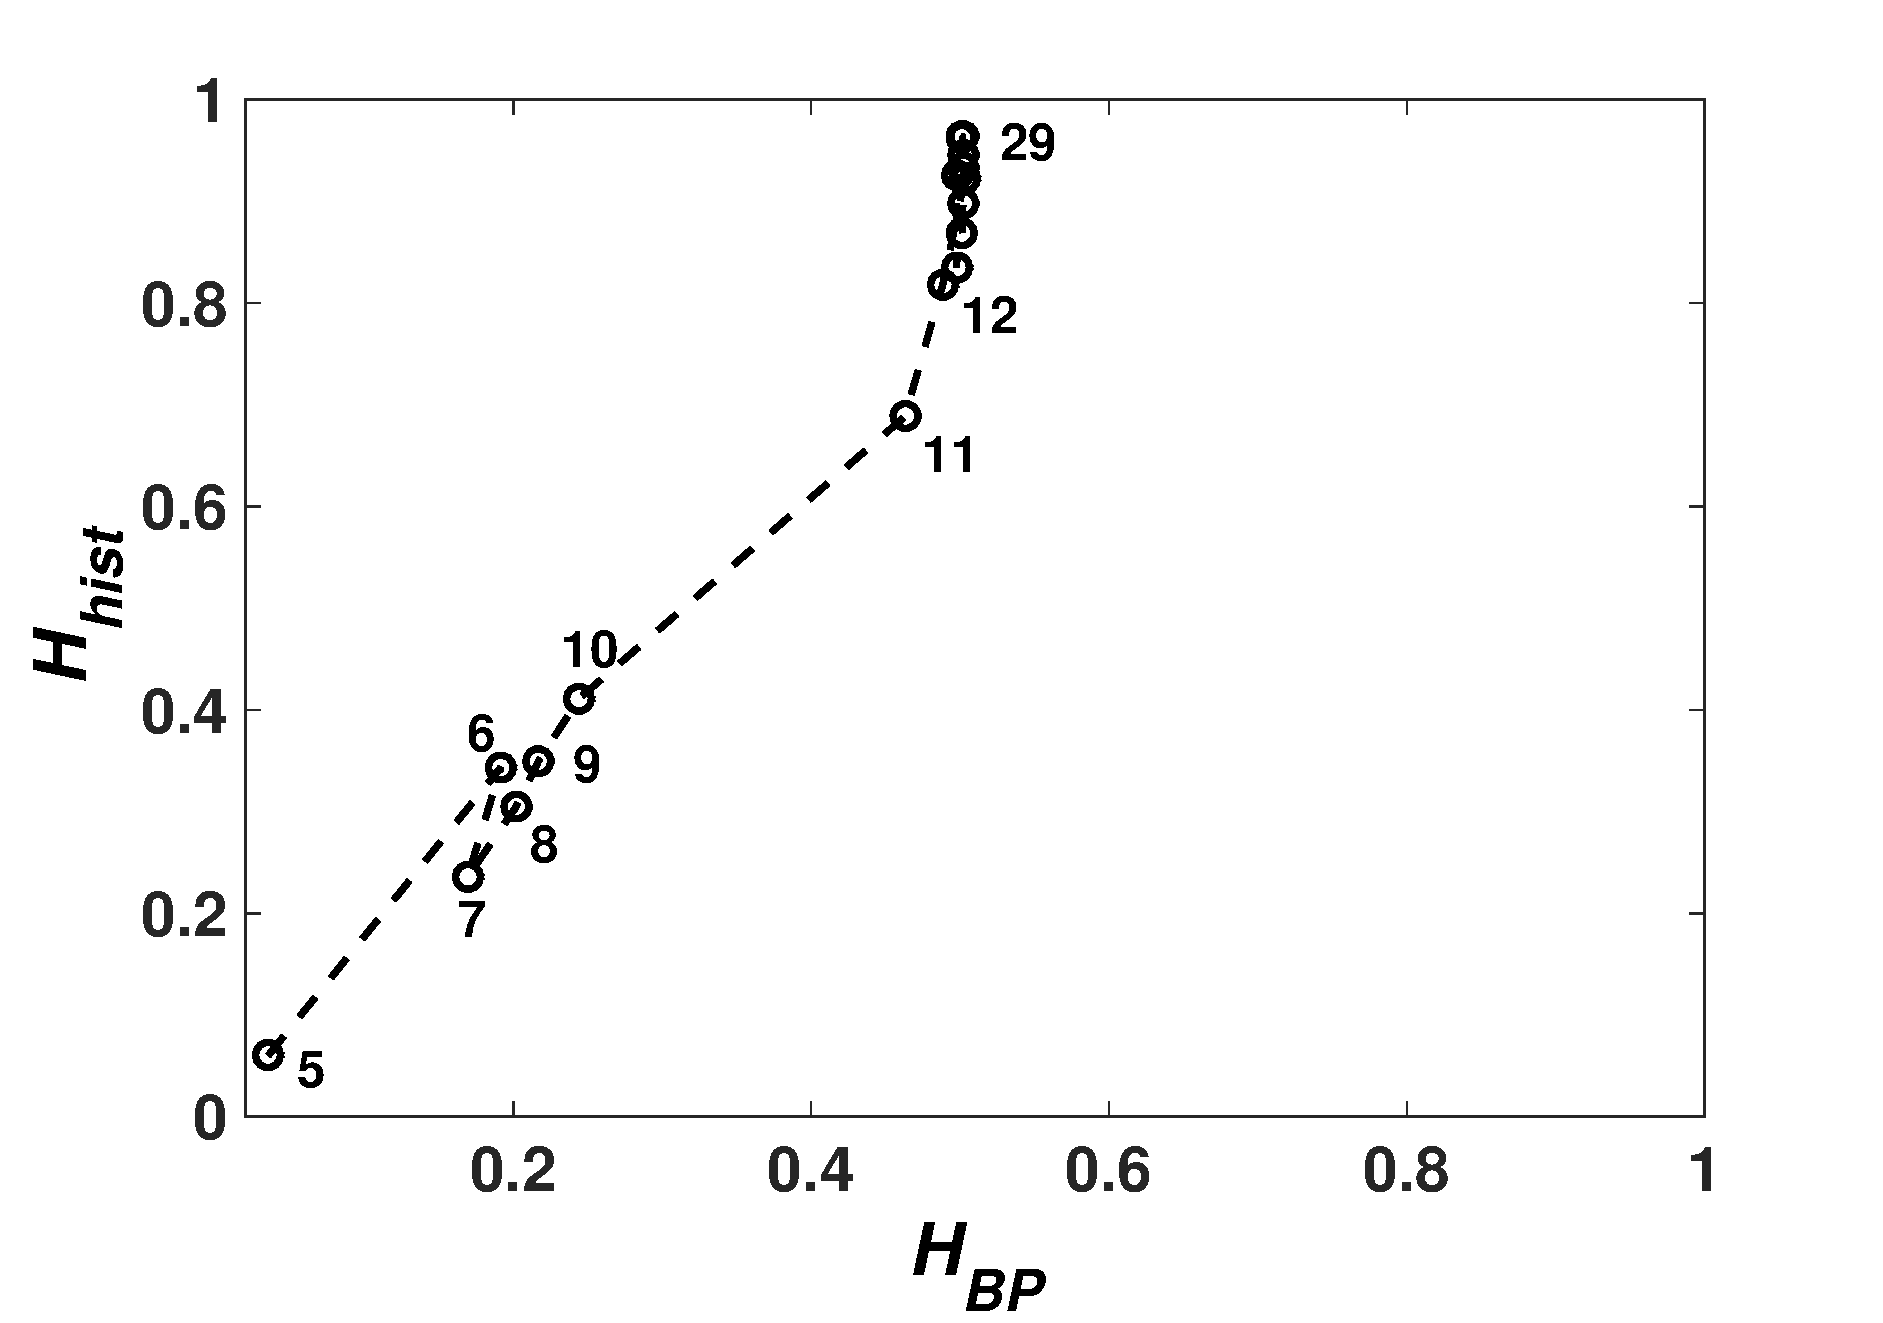
\includegraphics[width=0.7\columnwidth]{HBPvsHhist}\\
    \caption{Plane $H_{hist}$ - $H_{BP}$  for different number of bits. }\label{fig:HBPvsHhist}
\end{figure}


\begin{figure}
    \centering
        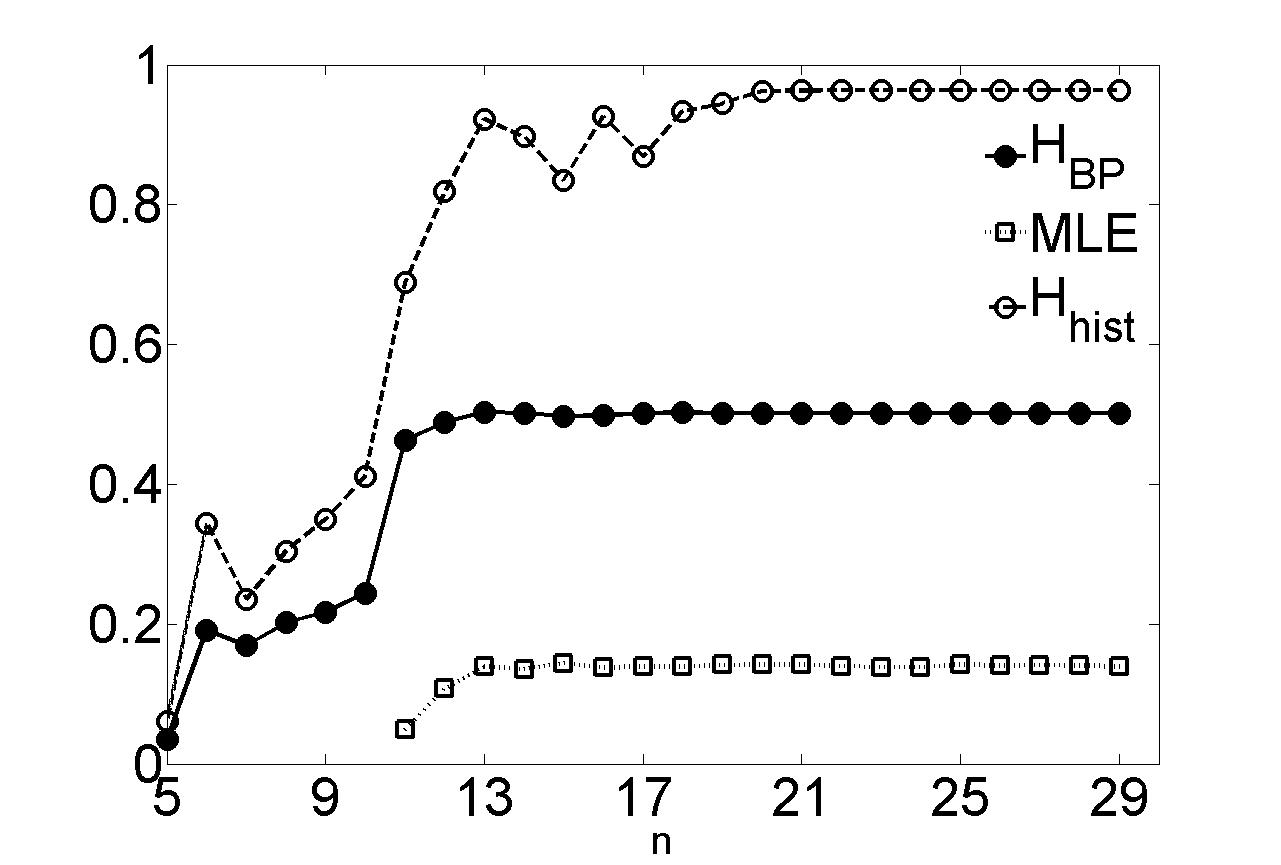
\includegraphics[width=0.7\columnwidth]{HBPHhist}\\
    \caption{Weighted average of quantifiers $H_{BP}$,  $H_{hist}$ and \textsl{MLE} as functions of the number of bits.}\label{fig:HBPHhist}
\end{figure}

Finally, Fig. \ref{puntos}.d shows the number of initial conditions that
presents periods $T$ higher and lower than $1,000$. Again, a value
of $12$ for $n_f$ seems to be the limit to obtain a good
approximation of the system.

Table \ref{tabla:MLE} shows the calculated \textsl{MLE} for some values of $n_f$. It can be seen that, as expected, while $n_f$ increases the \textsl{MLE} tends to its theoretical value.
 
\begin{table}[!t]\label{tabla:MLE}
\begin{center}
\caption{\textsl{MLE} for different values of $n_f$.}
\label{tabla:MLE}
\begin{tabular}{l l}

  \hline

  $n_f$ & \textsl{MLE} \\
  \hline
  \hline
  $11$ & $0.049214459144086$ \\
  $12$ & $0.107498218078192$ \\
  $13$ & $0.139472468153184$ \\
  $14$ & $ 0.135756935006498$ \\
  $15$ & $0.144155039896011$ \\
  $16$ & $0.137514471652835$ \\
  $25$ & $0.142134613438658$ \\
  $27$ & $0.141180317168284$ \\
  float & $0.142275657734227$ \\
   \hline

\end{tabular}
\end{center}

\end{table}

\section{Conclusion} \label{sec:conclusions}
In this work, we have developed a detailed analysis of the changes in behaviour of a $2D$-quadratic map fixed-point implementation. Results show that compared to floating-point, fixed-point arithmetic executed on an integer datapath has a limited impact on the attraction domain and, also, in the characteristics of the sequences generated by the digitalized maps. We have found a threshold for the required 
number of bits where the system keeps the properties of the original (real) one. Our goal is to report the rate of degradation for each property, so as to be used by authors at the time of designing their particular applications. 
This is interesting because in many applications these maps are intended to be used as controlled noise generators and this system, in particular, admits the development of a novel encryption system.


\section*{Acknowledgment}
This work was partially  supported  by  the  Consejo  Nacional de
Investigaciones Cient\'{\i}ficas y T\'ecnicas (CONICET), Argentina
(PIP 112-201101-00840), ANPCyT (PICT-2013-2066), UNMDP and the International Centre for Theoretical Physics (ICTP) Associateship Scheme.\\

% Bibliography
\bibliographystyle{ACM-Reference-Format}
\bibliography{BibPaperSprott}

\end{document}
